% dsa110-rt: narrative overview of the real-time FRB search pipeline.
% Compile: pdflatex -interaction=nonstopmode dsa110-rt-overview.tex
% (run twice for cross-references)

\documentclass[11pt,a4paper]{article}

% --- packages -----------------------------------------------------------------
\usepackage[T1]{fontenc}
\usepackage[utf8]{inputenc}
\usepackage[margin=22mm,top=20mm,bottom=22mm]{geometry}
\usepackage[expansion=false,protrusion=true]{microtype}
\usepackage{parskip}
\usepackage{amsmath,amssymb,mathtools}
\usepackage{booktabs}
\usepackage{tabularx}
\newcolumntype{L}{>{\raggedright\arraybackslash}X}
\usepackage{graphicx}
\usepackage{caption,subcaption}
\usepackage{enumitem}
\usepackage{xcolor}
\usepackage[hidelinks]{hyperref}
\usepackage{cleveref}
\usepackage{tikz}
\usepackage{listings}
\usepackage{fancyhdr}
\usepackage{titlesec}

\usetikzlibrary{positioning,arrows.meta,calc,fit,backgrounds,shapes.geometric,
                shapes.symbols,decorations.pathreplacing,patterns}

\definecolor{corrcol}{HTML}{1F77B4}
\definecolor{srchcol}{HTML}{2CA02C}
\definecolor{coordcol}{HTML}{9467BD}
\definecolor{moncol}{HTML}{D62728}
\definecolor{deferredcol}{HTML}{888888}
\definecolor{shmcol}{HTML}{8C564B}
\definecolor{codebg}{HTML}{F7F7F7}

% --- listings (code blocks) ---------------------------------------------------
\lstset{
  backgroundcolor=\color{codebg},
  basicstyle=\ttfamily\footnotesize,
  breaklines=true,
  frame=single,
  framerule=0pt,
  xleftmargin=0.5em,
  xrightmargin=0.5em,
  showstringspaces=false,
  columns=fullflexible,
}

% --- title block --------------------------------------------------------------
\title{\textbf{The DSA-110 real-time FRB search pipeline}\\[2mm]
       \large A narrative reference for \texttt{dsa110-rt}\\[1mm]
       \normalsize algorithms, data flow, statistics and noise
       estimation, control, monitoring, and development pathway}
\date{2026 June 10}

\pagestyle{fancy}
\fancyhf{}
\fancyhead[L]{\small DSA-110 \texttt{dsa110-rt} narrative overview}
\fancyhead[R]{\small\thepage}

\titleformat{\section}{\normalfont\Large\bfseries\color{corrcol}}{\thesection}{0.8em}{}
\titleformat{\subsection}{\normalfont\large\bfseries}{\thesubsection}{0.7em}{}

% --- macros -------------------------------------------------------------------
\newcommand{\Kdm}{K_\mathrm{DM}}
\newcommand{\nutop}{\nu_\mathrm{top}}
\newcommand{\nubot}{\nu_\mathrm{bot}}
\newcommand{\DM}{\mathrm{DM}}
\newcommand{\dnu}{\Delta\nu_\mathrm{ch}}
\newcommand{\specnum}{\textit{specnum}}
\newcommand{\corr}{\texttt{corr}}
\newcommand{\srch}{\texttt{search}}
% \codeword{...} renders fixed-width text and tolerates _ # $ % & ~ ^.
% (\detokenize re-produces every char as a category-12 literal.)
% \text{} wrapper makes \codeword safe in math mode too.
\newcommand{\codeword}[1]{\text{\ttfamily\small\detokenize{#1}}}

\begin{document}

\maketitle
\thispagestyle{empty}

\begin{center}
\fbox{\parbox{0.93\linewidth}{\small
\textbf{Scope.}  This is a narrative reference for the
DSA-110 real-time FRB search pipeline as implemented in the
\codeword{dsa110-rt} repository (HEAD of \codeword{main},
2026 June 10).  It describes the algorithms, the mathematical
operations on the data --- with particular attention to the
statistics and noise-estimation chain (\Cref{sec:stats}) --- the
control and monitoring infrastructure, and the development pathway
that brought the system on-sky through the M7.4 acceptance gate, the
M7.7 real-time performance campaign, and the June 2026
injection-calibration commissioning.  Tests, benchmarks, and
acceptance reports are deliberately \emph{out of scope} of this
document --- those live in \codeword{docs/M7.4_*.md} and
\codeword{docs/m7/}.  A Monte-Carlo analysis of the FRB
matched-filter S/N loss as a function of DM, given the production v2
DM plan, is given in~\Cref{sec:mcloss}.  A development pathway for
adding intelligence to the C1 detector follows in~\Cref{sec:c1path}.
}}
\end{center}

\begin{center}
\fbox{\parbox{0.93\linewidth}{\small
\textbf{Changes since the 2026-06-02 edition.}  This revision folds
in the June 3--10 wave of work; the body text has been rewritten
in place, so this box is a map, not a diff:
\begingroup\sloppy
\begin{itemize}[topsep=2pt,itemsep=2pt,leftmargin=*]
\item \emph{M7.7 search-side real-time campaign}
      (Section~\ref{sec:search}, \ref{sec:perf}): Option-A corr-side
      coarse-DM dedispersion, symmetric-shift padding (100\,\% fine-DM
      coverage), the fftshift fold into the combine kernel, the
      real-output \codeword{irfft2} imager, and the move to the
      big-block op-point ($T_\mathrm{det}=256$, cadence 192 samples
      $= 201.3$\,ms).  The fleet now sustains $\sim$166\,ms/cube
      ($\sim$17\,\% real-time headroom) with the full b1..b64 boxcar
      bank.  Carry-over re-imaging is implemented and validated but
      OFF in production.
\item \emph{Production DM plan v2}
      (\codeword{dm_plan_N8_dmmin100_tol1.6_v2.npz}): 272 fine trials
      over DM 100--2653\,pc\,cm$^{-3}$, 8 coarse trials, Levin
      tolerance 1.6.  The Monte-Carlo S/N-loss study
      (Section~\ref{sec:mcloss}) has been re-run against it.
\item \emph{Statistics and noise estimation}
      (new Section~\ref{sec:stats}): the full chain --- corr-side
      requantisation, Layer-1 $\sigma$-clipped per-trial
      normalisation, the fp16 overflow hazard and the
      \codeword{input_clip_sigma} hardening, Layer-2 per-kernel EMA
      with the $\sigma_\mathrm{max}$-ratio clamp + escape hatch,
      decode thresholds and false-alarm budget, the DM-smear floor
      and noise-colour de-rating, and the linear fluence$\to$S/N
      calibration --- is now documented in one place.
\item \emph{Static-sky removal} (Section~\ref{sec:corrfast}): the
      one-pole EMA is replaced by \codeword{StaticSkyMean}, a strictly
      causal $\sim$1.07\,s (8-block) sliding mean per coarse-DM trial
      --- the EMA's $\tau\!\approx\!134$\,s lagged the $\sim$6.9\,s/2$\pi$
      core fringe winding and left the sky largely unsubtracted.  A
      30\,s-cadence \emph{sky monitor} export images the running mean
      on the h23 dashboard with RA/Dec graticule + NVSS overlay.
\item \emph{Detector wing-decode fix} (Sections~\ref{sec:c1},
      \ref{sec:stats}): \codeword{n_kernel_max_t} is now derived from
      the loaded kernel bank (64 for the production b1..b64 bank, was
      hardcoded 128), restoring a $[32,224)$ scoring window that
      tiles the 192-sample cadence exactly.  The stale value silently
      dropped 33\,\% of all stream samples and produced low-S/N
      off-DM ``wing'' decodes for bursts landing in the blind region.
\item \emph{Candidate sky coordinates} (Section~\ref{sec:c1}):
      reported $(l, m)$ now use centred pixel offsets (origin at
      $n_\mathrm{grid}/2$), the row/column axes are correctly
      interpreted as $(m, l)$, and the pixel scale is computed
      exactly from the gridder's \codeword{cell_lambda}
      ($1.240\times10^{-4}$\,rad/pix, was hardcoded
      $1.5\times10^{-4}$).
\item \emph{Injection system overhaul} (Section~\ref{sec:inject}):
      the injector's profile normalisation now follows the physical
      voltage $=\sqrt{\text{instantaneous flux}}$ convention (S/N
      $\propto F/\sqrt{W}$; the old unit-area convention delivered
      $F/W^{5/2}$); S/N calibration uses a \emph{linear} model
      $\mathrm{S/N} = K F/\sqrt{W}$ with width-independent per-DM
      buckets, a saturation-aware fluence ladder, probe-position
      rotation, and a pre-flight health check; the C2 matcher gates
      on specnum proximity with a wall-clock fallback; auto-arm uses
      a 32-block margin with monitor-staleness extrapolation; the
      \codeword{OnlineInjector} counts clean/partial/never-applied
      injections.
\item \emph{Search-side robustness (T1--T8, 2026-06-07/09)}:
      $\sigma_k$ clamp + escape hatch with per-kernel monitor points,
      bounded cube uploader, calibration-probe metering exemption,
      dump-health monitor points, C2 startup-grace pre-expiry
      tightening, event directories created only when the full cube
      set lands, \codeword{cube_ring_depth} 16$\to$12 + staggered
      spawn to fix the n09/n13 pinned-memory OOM.
\item \emph{C2 plotter} (Section~\ref{sec:c2}): the per-event
      \codeword{dm_time} figure is now a single contiguous-DM
      waterfall stacking all eight cubes, with robust per-row
      MAD normalisation.
\end{itemize}
\endgroup
}}
\end{center}

\tableofcontents

% =============================================================================
\section{Introduction}
\label{sec:intro}

The DSA-110 is a 110-element radio interferometer at the Owens
Valley Radio Observatory operating in the 1.31--1.50\,GHz band.
\codeword{dsa110-rt} is the real-time pipeline that turns the
SNAP F-engine packet stream into FRB candidates with a continuously
sustained, real-time-correct latency budget.  Two cadences govern
the data plane.  On the \emph{corr side} the controlling number is
the \emph{block cadence}
\[
   T_\mathrm{blk} = 4096\,\text{native samples}
   = 4096 \times \tau_\mathrm{nat}
   = 4096 \times 32.768~\mu\mathrm{s}
   = 0.134217728~\mathrm{s},
\]
i.e.\ 134.218\,ms per block; the corr-side hot path
(\codeword{corr_fast_integration}) runs at
$\mathrm{p50}\!\approx\!110\,\mathrm{ms}$,
$\mathrm{p99}\!\approx\!110.5\,\mathrm{ms}$ on the production fleet
(\codeword{docs/m72/M72_MORNING_REPORT_2026-05-20.md}).  On the
\emph{search side} the controlling number is the \emph{cube
cadence}: each detector cube spans $T_\mathrm{det}=256$ search
samples and advances by 192 samples of
$t_\mathrm{int}^\mathrm{search}=1048.576\,\mu$s, i.e.
\[
   T_\mathrm{cube} = 192 \times 1.048576~\mathrm{ms}
   = 201.327~\mathrm{ms}
   \quad\Longleftrightarrow\quad
   f_\mathrm{cube} = 4.967~\mathrm{cubes/s}.
\]
After the M7.7 performance campaign (Option-A corr-side coarse-DM
dedispersion, symmetric-shift padding, the fftshift fold, and the
real-output \codeword{irfft2} imager --- Section~\ref{sec:perf}) a
search half sustains $\sim$166\,ms/cube ($\sim$5.2--6.0 cubes/s
measured live), i.e.\ $\sim$17\,\% of real-time headroom with the
full 7-octave boxcar bank.

The pipeline runs on 16 correlator nodes (\codeword{n03}--\codeword{n22},
with gaps), 4 search nodes (\codeword{n01}, \codeword{n02},
\codeword{n09}, \codeword{n13}), and an operations host \codeword{h23}
that runs the operator dashboard, the C2 coincidencer, and the legacy
slow-vis archive consumers.  A second operations host
\codeword{lxd110h20} runs the InfluxDB / Grafana stack.

\Cref{fig:topfig} shows the top-level data flow and the responsibilities
of each host class.

\begin{figure}[ht]
\centering
\resizebox{\textwidth}{!}{%
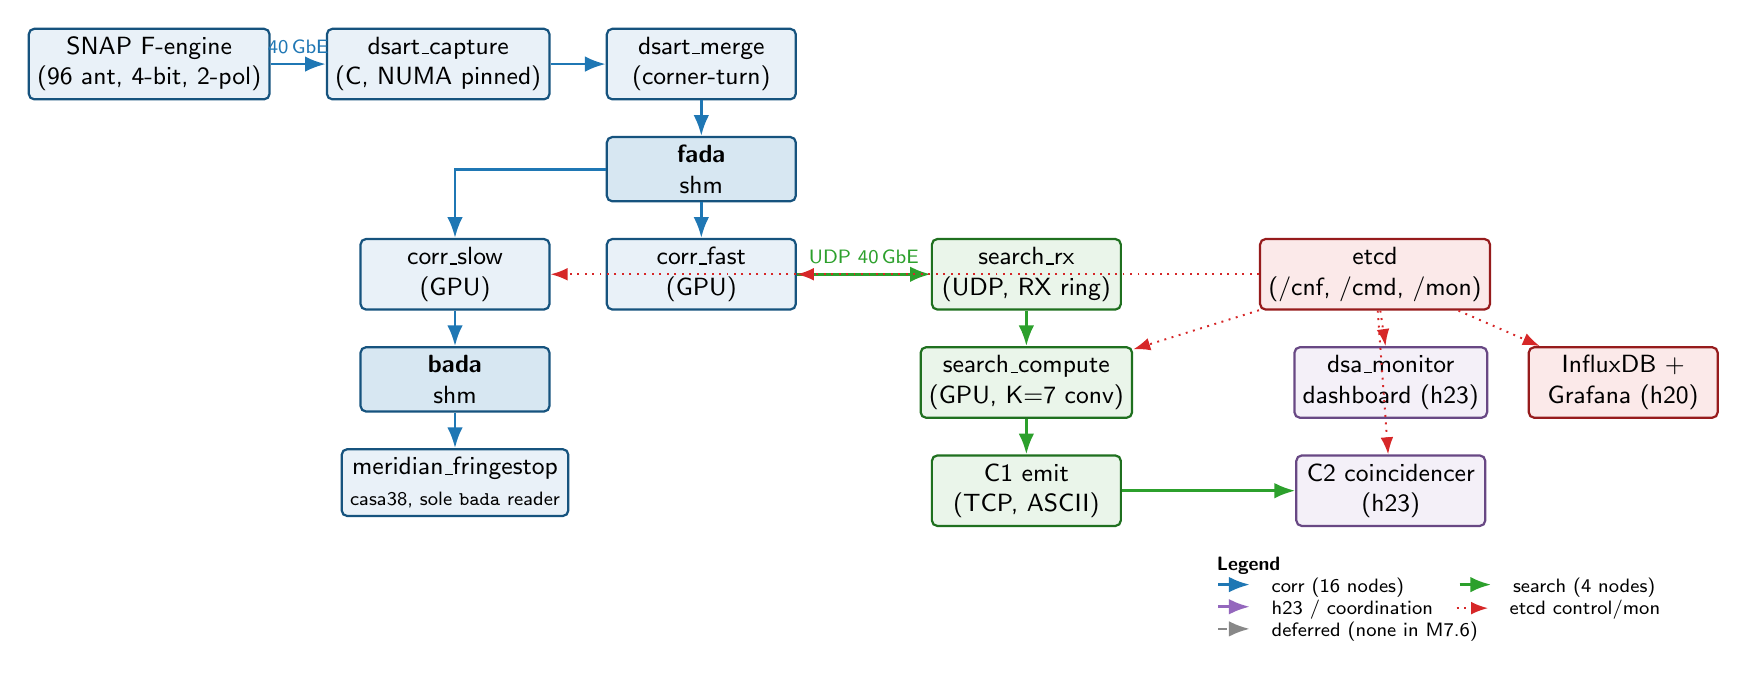
\begin{tikzpicture}[
   font=\sffamily\small,
   node distance=4.5mm and 7mm,
   box/.style={draw,rounded corners=2pt,minimum height=8mm,inner sep=3pt,
               minimum width=24mm,align=center,fill=#1!10,draw=#1!70!black},
   thick,>=Latex,
]
\node[box=corrcol] (snap) {SNAP F-engine\\(96 ant, 4-bit, 2-pol)};
\node[box=corrcol, right=of snap] (cap) {dsart\_capture\\(C, NUMA pinned)};
\node[box=corrcol, right=of cap]  (mrg) {dsart\_merge\\(corner-turn)};
\node[box=corrcol, below=of mrg, fill=corrcol!18] (fad) {\textbf{fada}\\ shm};
\node[box=corrcol, below=of fad] (cf) {corr\_fast\\(GPU)};
\node[box=corrcol, left=of cf] (cs) {corr\_slow\\(GPU)};
\node[box=corrcol, below=of cs, fill=corrcol!18] (bada) {\textbf{bada}\\ shm};
\node[box=corrcol, below=of bada] (mfs)
        {meridian\_fringestop\\ {\scriptsize casa38, sole \texttt{bada} reader}};
\node[box=srchcol, right=of cf, xshift=10mm] (rx) {search\_rx\\(UDP, RX ring)};
\node[box=srchcol, below=of rx] (sc) {search\_compute\\(GPU, K=7 conv)};
\node[box=srchcol, below=of sc] (c1) {C1 emit\\(TCP, ASCII)};
\node[box=coordcol, right=of c1, xshift=15mm] (c2) {C2 coincidencer\\(h23)};
\node[box=coordcol, above=of c2] (dash) {dsa\_monitor\\dashboard (h23)};
\node[box=moncol, above=of dash, xshift=-2mm] (etcd) {etcd\\(/cnf, /cmd, /mon)};
\node[box=moncol, right=of dash, xshift=-2mm] (inf) {InfluxDB +\\Grafana (h20)};

% data-plane arrows
\draw[->,corrcol,line width=1.0pt] (snap) -- (cap) node[midway,above]{\scriptsize 40\,GbE};
\draw[->,corrcol,line width=1.0pt] (cap)  -- (mrg);
\draw[->,corrcol,line width=1.0pt] (mrg)  -- (fad);
\draw[->,corrcol,line width=1.0pt] (fad)  -- (cf);
\draw[->,corrcol,line width=1.0pt] (fad)  -| (cs);
\draw[->,corrcol,line width=1.0pt] (cs)   -- (bada);
\draw[->,corrcol,line width=1.0pt] (bada) -- (mfs);
\draw[->,srchcol,line width=1.0pt]
        (cf.east) .. controls +(0.7cm,0) and +(-0.7cm,0) .. (rx.west)
        node[midway,above]{\scriptsize UDP 40\,GbE};
\draw[->,srchcol,line width=1.0pt] (rx) -- (sc);
\draw[->,srchcol,line width=1.0pt] (sc) -- (c1);
\draw[->,srchcol,line width=1.0pt] (c1) -- (c2);

% control-plane arrows (etcd / mon)
\draw[->,moncol,dotted,line width=0.7pt] (etcd) -- (cf);
\draw[->,moncol,dotted,line width=0.7pt] (etcd) -- (cs);
\draw[->,moncol,dotted,line width=0.7pt] (etcd) -- (sc);
\draw[->,moncol,dotted,line width=0.7pt] (etcd) -- (c2);
\draw[->,moncol,dotted,line width=0.7pt] (etcd) -- (dash);
\draw[->,moncol,dotted,line width=0.7pt] (etcd) -- (inf);

% legend
\node[anchor=west,font=\sffamily\scriptsize] at (snap.south west) {\quad};
\node[anchor=north west,font=\sffamily\scriptsize,fill=white,inner sep=2pt,
      align=left]
        at ($(c2.south east) + (-3.5cm,-3mm)$) {
        \textbf{Legend}\\
        \tikz \draw[corrcol,line width=1.0pt,->] (0,0) -- (4mm,0); ~ corr (16 nodes)\hspace{6mm}
        \tikz \draw[srchcol,line width=1.0pt,->] (0,0) -- (4mm,0); ~ search (4 nodes)\\
        \tikz \draw[coordcol,line width=1.0pt,->] (0,0) -- (4mm,0); ~ h23 / coordination\hspace{2mm}
        \tikz \draw[moncol,line width=0.7pt,dotted,->] (0,0) -- (4mm,0); ~ etcd control/mon\\
        \tikz \draw[deferredcol,dashed,line width=1pt,->] (0,0) -- (4mm,0); ~ deferred (none in M7.6)};

\end{tikzpicture}
}% end resizebox
\caption{Top-level topology of \texttt{dsa110-rt}.  Per-block (134\,ms) data
flow is in solid arrows; control and monitoring traffic in red dotted arrows.
The slow-vis sink \texttt{meridian\_fringestop} consumes \texttt{bada} via
PSRDADA and is now the sole \texttt{bada} reader, run from the casa38
environment via the operator-side wrapper
\texttt{tools/ops/meridian\_fringestop\_rt.py} (M7.4 Phase~9, 2026-05-30).}
\label{fig:topfig}
\end{figure}


% =============================================================================
\section{Numerical conventions and the band}
\label{sec:numconv}

The configured SNAP band has $f_0 = 1.530$\,GHz on its top edge and a
total bandwidth of $250$\,MHz across $8192$ native channels, hence
$\dnu = 30.517578125$\,kHz / channel.  We process only a contiguous
$6144$-channel sub-band from system channel $1024$ down to system
channel $7167$ inclusive; with the edge convention pinned in
\codeword{src/dsart/common/constants.py::freq_GHz}, the processed
band is
\[
\nutop = 1.49875~\mathrm{GHz},\qquad
\nubot = 1.311280517578125~\mathrm{GHz},\qquad
\mathrm{BW}_\mathrm{proc} = 187.469~\mathrm{MHz}.
\]
The 6144 native channels are sliced into $N_\mathrm{cg}=16$
\emph{chgroups} of $384$ channels each --- one chgroup per correlator
node.  Channels are stored \emph{descending} in frequency: local
channel 0 is the highest frequency in its chgroup, local channel 383
the lowest.

Time bookkeeping is by SNAP \emph{specnum}, a 16-bit packet sequence
counter where 1 specnum $= 2$ native samples $= 65.536\,\mu$s.  A
PSRDADA block holds $2048$ specnums $= 4096$ native samples
$= 134.218$\,ms.

\paragraph{Dispersion constant.}
The pipeline uses the standard pulsar-astronomy dispersion constant
\begin{equation}
\tau(\nu,\DM) = \Kdm \cdot \DM / \nu^2,
\qquad
\Kdm = 4.148808~\mathrm{ms}\,\mathrm{GHz}^2\,\mathrm{pc}^{-1}\,\mathrm{cm}^{3},
\label{eq:taudm}
\end{equation}
matching \codeword{src/dsart/common/constants.K_DM_MS_GHZ2_PC} and
the legacy \codeword{gen_dmtrials.py} reference.  At
$\DM=3000\,\mathrm{pc\,cm^{-3}}$ the processed-band sweep is
$\Delta\tau = \Kdm \cdot 3000 \cdot (1/\nubot^2 - 1/\nutop^2)
        \approx 1697.5$\,ms.

\paragraph{Polarisations.}  Voltages and per-pol RFI statistics carry
two polarisations (XX, YY); the calibration / RFI / fast-GEMM stack
operates per-pol.  Immediately after the fast correlator, the two
polarisations are summed to a single Stokes-I product
($V_I = V_\mathrm{XX} + V_\mathrm{YY}$) and the entire search path
(gridding, dedispersion, imaging, detection) is single-polarisation.

\paragraph{Antennas and baselines.}  $N_\mathrm{ant} = 96$ antennas
after the F-engine map; the upper-triangle baseline count
\emph{including} the auto-correlations is
$N_\mathrm{bl} = 96\cdot97/2 = 4656$, fixed in
\codeword{common.constants.NBASE}.

\paragraph{Operating points.}
The production operating point integrates fast-correlator output to
$t_\mathrm{int}^\mathrm{fast} = t_\mathrm{int}^\mathrm{search}
= 1048.576\,\mu$s (32 $\times$ native) and bakes a corr-side
$8\times$ channel-sum into the wire format, so the search-side
fine-DM combiner sees $768$ frequency channels of
$\Delta\nu = 244.140$\,kHz each.  The production DM plan is the v2
\codeword{dm_plan_N8_dmmin100_tol1.6_v2.npz}: $N_\mathrm{fine}=272$
trials over DM 100--2653\,pc\,cm$^{-3}$, $N_\mathrm{coarse}=8$
(one per search GPU half), Levin tolerance $\theta=1.6$, fine-trial
spacing 9.34--9.58\,pc\,cm$^{-3}$.  Both numbers matter for the S/N
analysis in~\Cref{sec:mcloss}.


% =============================================================================
\section{Data flow and host topology}
\label{sec:dataflow}

\Cref{fig:nodeflow} expands~\Cref{fig:topfig} to the level of routines
on one corr node and one search node.  Each routine is a separately
addressable POSIX process spawned by the \codeword{dsart_rt} per-node
orchestrator (the user-systemd unit
\codeword{dsart-rt.service}; see~\Cref{sec:control}).  Inter-routine
data is exchanged through PSRDADA shared-memory ring buffers (named
\codeword{fada} / \codeword{dada} / \codeword{eada} / \codeword{bada}
following the legacy naming) and, for the M7.6 RFI window monitor,
through a custom POSIX-shm ring (\codeword{/dev/shm/dsart-rfi-window-<cn>}).

\begin{figure}[ht]
\centering
\resizebox{\textwidth}{!}{%
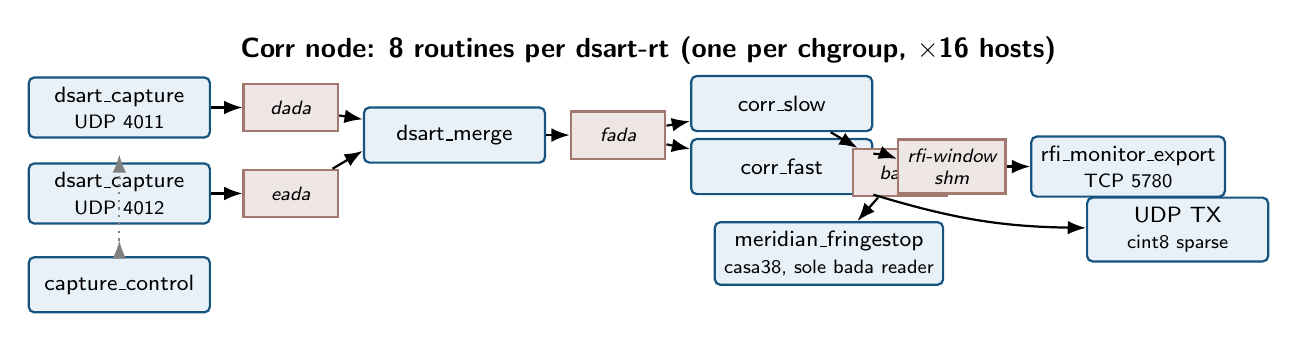
\begin{tikzpicture}[font=\sffamily\footnotesize,
   rt/.style={draw,rounded corners=2pt,minimum width=23mm,
              minimum height=7mm,fill=corrcol!10,draw=corrcol!70!black,align=center},
   srt/.style={draw,rounded corners=2pt,minimum width=23mm,
              minimum height=7mm,fill=srchcol!10,draw=srchcol!70!black,align=center},
   shm/.style={draw,thick,fill=shmcol!15,draw=shmcol!80,minimum width=12mm,
              minimum height=6mm,align=center,font=\sffamily\scriptsize\itshape},
   thick,>=Latex,
   node distance=3mm,
]
% ----- left: one corr node
\node[rt] (capa) at (0,0)        {dsart\_capture\\ \scriptsize UDP 4011};
\node[rt,below=of capa] (capb)   {dsart\_capture\\ \scriptsize UDP 4012};
\node[rt,below=4mm of capb] (cctl){capture\_control};
\node[shm,right=4mm of capa] (dada) {dada};
\node[shm,right=4mm of capb] (eada) {eada};
\node[rt,right=of dada,yshift=-3.5mm] (merge) {dsart\_merge};
\node[shm,right=of merge] (fada) {fada};
\node[rt,right=of fada,yshift=4mm] (cslow) {corr\_slow};
\node[rt,right=of fada,yshift=-4mm] (cfast) {corr\_fast};
\node[shm,below=2mm of cslow,xshift=15mm] (bada) {bada};
\node[shm,right=of cfast] (rfishm) {rfi-window\\shm};
\node[rt,right=of rfishm] (rfimon){rfi\_monitor\_export\\ \scriptsize TCP 5780};
% meridian_fringestop is now the sole bada reader (Phase 9, 2026-05-30);
% the legacy dada_drain stand-in is retired.
\node[rt,below=of bada,xshift=-9mm] (mfs)
   {meridian\_fringestop\\ \scriptsize casa38, sole bada reader};

% UDP TX
\node[rt,right=of cfast,xshift=24mm,yshift=-8mm] (tx) {UDP TX\\ \scriptsize cint8 sparse};

% wires
\draw[->] (capa) -- (dada);
\draw[->] (capb) -- (eada);
\draw[->] (dada) -- ([yshift= 2mm]merge.west);
\draw[->] (eada) -- ([yshift=-2mm]merge.west);
\draw[->] (merge) -- (fada);
\draw[->] (fada) -- (cslow);
\draw[->] (fada) -- (cfast);
\draw[->] (cslow) -- (bada);
\draw[->] (bada) -- (mfs);
\draw[->,thick,bend left=8] (cfast) to (rfishm);
\draw[->,thick] (rfishm) -- (rfimon);
\draw[->,thick,bend right=8] (cfast) to (tx);
\draw[->,dotted,gray] (cctl) -- ([yshift=-2mm]capa.south);
\draw[->,dotted,gray] (cctl) -- ([yshift=-2mm]capb.south);

% ----- title
\node[font=\sffamily\bfseries,anchor=south] at (current bounding box.north)
    {Corr node: 8 routines per dsart-rt (one per chgroup, $\times$16 hosts)};
\end{tikzpicture}
}% end resizebox

\vspace{4mm}

\resizebox{\textwidth}{!}{%
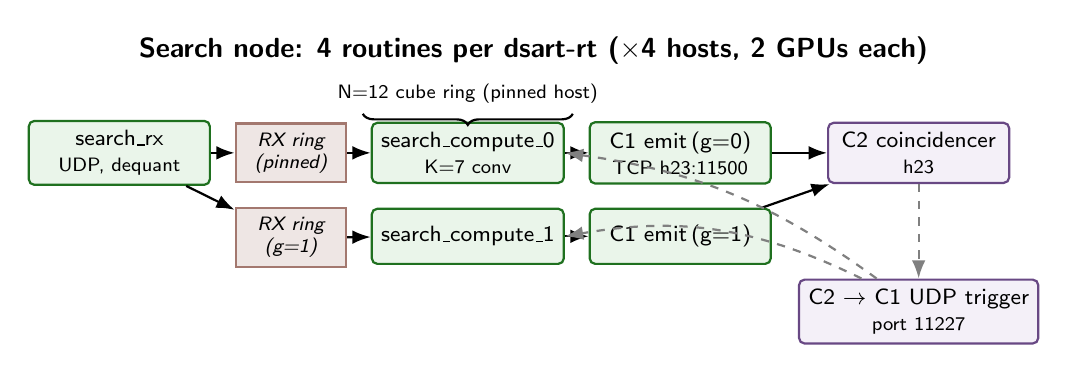
\begin{tikzpicture}[font=\sffamily\footnotesize,
   srt/.style={draw,rounded corners=2pt,minimum width=23mm,minimum height=7mm,
              fill=srchcol!10,draw=srchcol!70!black,align=center},
   shm/.style={draw,thick,fill=shmcol!15,draw=shmcol!80,minimum width=14mm,
              minimum height=6mm,align=center,font=\sffamily\scriptsize\itshape},
   coord/.style={draw,rounded corners=2pt,minimum width=23mm,minimum height=7mm,
              fill=coordcol!10,draw=coordcol!70!black,align=center},
   thick,>=Latex,node distance=3mm,
]
\node[srt] (rx) at (0,0)    {search\_rx\\ \scriptsize UDP, dequant};
\node[shm,right=of rx] (ring) {RX ring\\ (pinned)};
\node[srt,right=of ring] (sc0) {search\_compute\_0\\ \scriptsize K=7 conv};
\node[srt,below=of sc0] (sc1) {search\_compute\_1};
\node[srt,right=of sc0] (c1a) {C1 emit\,(g=0)\\ \scriptsize TCP h23:11500};
\node[srt,right=of sc1] (c1b) {C1 emit\,(g=1)};
\node[shm,below=of ring] (ringg){RX ring\\ (g=1)};
\node[coord,right=of c1a,xshift=4mm] (c2) {C2 coincidencer\\ \scriptsize h23};

\draw[->] (rx) -- (ring);
\draw[->] (rx) -- (ringg);
\draw[->] (ring) -- (sc0);
\draw[->] (ringg) -- (sc1);
\draw[->] (sc0) -- (c1a);
\draw[->] (sc1) -- (c1b);
\draw[->] (c1a) -- (c2);
\draw[->] (c1b) -- (c2);

\node[srt,below=12mm of c2,fill=coordcol!10,draw=coordcol!70!black]
     (trig) {C2 $\rightarrow$ C1 UDP trigger\\ \scriptsize port 11227};
\draw[->,gray,dashed] (c2) -- (trig);
\draw[->,gray,dashed,bend right=14] (trig) to (sc0.east);
\draw[->,gray,dashed,bend right=18] (trig) to (sc1.east);

% N=8 cube retention ring shown as bracket
\draw[decorate,decoration={brace,amplitude=4pt}]
    ($(sc0.north east)+(0.1,0.1)$) -- ($(sc0.north west)+(-0.1,0.1)$)
    node[midway,above,font=\sffamily\scriptsize]
    {N=12 cube ring (pinned host)};

\node[font=\sffamily\bfseries,anchor=south] at (current bounding box.north)
   {Search node: 4 routines per dsart-rt ($\times$4 hosts, 2 GPUs each)};
\end{tikzpicture}
}% end resizebox

\caption{Routine-level data flow on (top) one of 16 corr nodes and
(bottom) one of 4 search nodes.  Brown shapes are shared-memory
buffers.  Dashed grey is the C2$\rightarrow$C1 UDP trigger fan-out
(\codeword{cube_dump} on demand).  The dada\_drain routine is the
PSRDADA reference reader needed to keep the multi-reader \texttt{fada}
buffer from blocking when the slow path is idle.}
\label{fig:nodeflow}
\end{figure}

The numerical tower at each hop is summarised in
\Cref{tab:requant}.  Every requantisation is documented in
\codeword{src/dsart/common/contracts.py} and pinned in
\codeword{src/dsart/common/constants.py}.

\begin{table}[ht]
\centering
\caption{Numerical tower per hop.  Sizes are per 134\,ms block on
one corr node (one of 16 chgroups), unless noted.  Stokes-I sum
runs on the GPU before any quantisation.}
\label{tab:requant}
\small
\begin{tabular}{lllll}
\toprule
Stage & Tensor & Dtype & Shape per block & Notes \\
\midrule
SNAP packet payload      & $E_i^p(\nu,t)$ & 4-bit cplx & $96\!\times\!384\!\times\!2048\!\times\!2$ &
   nibble pack; multiplied by $0.05$ on unpack \\
\codeword{fada} merged   & $E_i^p(\nu,t)$ & 4-bit cplx & same                                      &
   reassembled, 32 SNAP shards $\rightarrow$ contiguous \\
Unpack on GPU           & $E_i^p(\nu,t)$ & fp16 cplx  & same                                      &
   $\times 0.05$ scale baked into kernel \\
Autos / RFI stats       & $S_1, S_2$    & fp32        & $96\!\times\!384\!\times\!2 \times |M|$    &
   $M\in\{64,256,1024,4096\}$ for SK aggregation \\
Cal-apply               & $E_i^p$       & fp16 cplx   & same                                      &
   $E \leftarrow E\,g_i\,b_i(\nu)\,(1-\text{mask})$ \\
Fast GEMM (X-engine)    & $V_{ij}^{p}$  & fp32$\rightarrow$cfp16 & $4656\!\times\!384\!\times\!2 \times t/8$ &
   fp16 GEMM, fp32 accum, cast on store \\
Stokes-I sum            & $V_I$         & cfp16       & $4656\!\times\!384 \times t/8$            &
   $V_I = V_\mathrm{XX}+V_\mathrm{YY}$ \\
Chan-sum $\times 8$      & $V_I$         & cfp16       & $4656\!\times\!48 \times t/8$             &
   M7.3 production only \\
Coarse-DM dedispersion (Option A) & $V_I'$  & cfp32        & per coarse-DM trial                       &
   per-(ch, $\DM_c$) integer shifts; 2-block sliding window \\
Gridder accum           & $G_I(u,v)$    & cfp32        & sparse-COO $\sim$5800 cells              &
   meridian-transit (u,v) only; \textbf{no fringe-stop} on fast path \\
Static-sky mean         & $G_I - \overline{G_I}$ & cfp32 & per coarse-DM trial & strictly causal 8-block ($\approx$1.07\,s) sliding mean \\
Sparse-COO gather       & nnz, $G_I'$   & cint8        & $\sim$5800 cells $\times$ 8 coarse DMs &
   per-(dm, t)-tile quantise, $\mathrm{scale} = \max|x|/127$ \\
UDP TX                  & on-wire      & cint8 + 72-B hdr & one packet per coarse-DM             &
   per-cube sequence numbering, sparse pattern id \\
RX dequantise           & $G_I'$        & fp16 cplx   & $\sim$5800$\times 8$                       &
   reverse scale; assemble per-chgroup slabs \\
Fine-DM combiner        & $G_{I,f}'$    & fp16 cplx   & $34\times256\times256\times t$ per half &
   $\delta\!\DM$ integer shifts per chgroup, signed; sym-shift padded \\
Imager                  & $I(l,m)$     & fp16 real   & same                                       &
   $I = \mathrm{irFFT}_2(G_{I,f}')$, fftshift folded into combine \\
Detector                & $c_k$         & fp16 / fp32 score & $K=7$ kernels (b1..b64)              &
   per-kernel boxcar via cumsum diff \\
\bottomrule
\end{tabular}
\end{table}


% =============================================================================
\section{The corr-side hot path}
\label{sec:corrfast}

\subsection{From SNAP to \texttt{fada}}

Two C binaries per corr node each consume one SNAP fan-out
(\codeword{dsart_capture_manythread}, ports 4011 and 4012).  They
NUMA-pin themselves to the GPU socket, validate the SNAP transport
header (magic, version, channel range), and shard incoming packets
into \codeword{dada} / \codeword{eada} PSRDADA rings of $r=N$
multi-reader depth.  A small Python sidecar
(\codeword{dsart.services.capture_control}) publishes per-port
cumulative counters (\codeword{n_recv_packets},
\codeword{n_dropped_payload}, \codeword{n_too_late}, \dots) into
the etcd key \codeword{/mon/corr_rt/<cn>/capture/<udp_port>}; the
M7.6 InfluxDB pusher converts these to per-second deltas (see
\Cref{sec:control}).

A third routine, \codeword{dsart_merge} (C, single-thread), reads
both shards and corner-turns the SNAP fan-out into the canonical
$[t,\,96,\,384,\,2]$ voltage tensor, written into the \codeword{fada}
ring.  \codeword{fada} is the only multi-reader buffer in the data
plane: it is consumed in parallel by \codeword{corr_slow} (slow
visibilities) and \codeword{corr_fast} (fast visibilities for the
search path).  The \codeword{bada} ring on the other side of
\codeword{corr_slow} is now drained directly by
\codeword{meridian_fringestop} (sole \codeword{bada} reader,
Section~\ref{sec:mfs}); the historical \codeword{bada_drain} /
\codeword{dada_drain} stand-in that used to backstop a missing slow-vis
consumer was removed in M7.4 Phase~9.

\subsection{\texttt{corr\_slow}: full-resolution visibilities}

\codeword{corr_slow} runs an fp32 X-engine over the full 96-antenna
upper triangle every block.  The output is a
$[4656,\,384,\,2]$~complex64 visibility tensor pushed into the
\codeword{bada} PSRDADA buffer.  This is byte-for-byte the legacy
\codeword{bada} contract preserved across the upgrade (see
\Cref{sec:legacy}) so the \codeword{meridian_fringestop} consumer
can be reattached without any code change.

\subsection{\texttt{corr\_fast}: RFI, calibration, GEMM, gridding, dedispersion}

\codeword{corr_fast_integration} is the production hot path.  All
GPU work runs on a single CUDA stream so the per-block budget can
be measured with one Event pair.  The pipeline is the following ten
steps, in order:

\begin{enumerate}[topsep=2pt,itemsep=2pt]
\item \textbf{Unpack} 4-bit nibbles to fp16, multiplying by the SNAP
    LSB scale $0.05$ in the same kernel.  Tensor layout:
    $E_i^p(\nu, t)$ as $[N_\mathrm{ant},\,N_\mathrm{ch},\,N_t,\,N_\mathrm{pol}]$.

\item \textbf{Autos} $S_1, S_2$ over native-time aggregation factors
    $M \in \{64,256,1024,4096\}$.  These feed the RFI flagger and
    the M7.6 RFI window aggregator.

\item \textbf{RFI flagging} (per pol, per chgroup, see~\Cref{sec:rfi}).
    Output is a per-cell binary mask $\mathcal{M}_i(\nu,t,p) \in \{0,1\}$
    plus a per-cell \codeword{source_tag} bitfield naming which detectors
    fired.

\item \textbf{Calibration apply}.  Per-antenna gain $g_i$, per-channel
    bandpass $b_i(\nu)$, and the RFI mask combine into a single complex
    weight applied in-place:
    \[
       E_i^p(\nu,t) \;\leftarrow\; g_i \cdot b_i^p(\nu) \cdot
                                   (1 - \mathcal{M}_i(\nu,t,p))
                                   \cdot E_i^p(\nu,t).
    \]
    Flagged cells thus contribute a hard zero into the X-engine.  Note
    that the bandpass calibration is broadcast per-chgroup from a single
    cal solution per node; the design value of 48 chans per cal point
    is decimated $\times 8$ from the channels at sky.
    \emph{Injection hook (step 4b)}: if the orchestrator was launched
    with \codeword{--inject-watch} (the production default), an
    etcd-driven \codeword{OnlineInjector} mutates the calibrated
    voltages in place to add any synthetic FRBs whose dispersed
    footprint overlaps this block
    (\codeword{_apply_online_injection},
    \codeword{corr_fast_integration.py:1704}; full mechanics in
    Section~\ref{sec:inject}).  The call is a single
    \codeword{torch.Tensor.add_} on the live voltage tensor --- zero
    allocation, zero copy --- and a single \codeword{is None} test on
    the no-inject path.  M7.4 Phase~8 (2026-05-28) moved this hook from
    pre-RFI to post-cal so the per-antenna fringe of an injected point
    source lands in the calibrated array frame; the previous pre-cal
    placement let \codeword{apply_cal_split} rotate each antenna's
    injected phase by its calibration solution, smearing the source
    away from the requested $(l,m)$.

\item \textbf{Correlation}.  A custom fp16 GEMM over the upper-triangle
    baseline list computes
    \begin{equation}
    V_{ij}^p(\nu,t) = \sum_{t'\,\in\,\text{int}} E_i^{p*}(\nu,t')\,E_j^p(\nu,t'),
    \quad i\le j,
    \label{eq:corr}
    \end{equation}
    summed over $t_\mathrm{int}^\mathrm{fast} = 8$ native samples
    (default operating point).  Accumulators are fp32, output is
    cfp16.  No diagonal special-casing.

\item \textbf{Stokes-I sum on GPU}.  $V_I = V_\mathrm{XX}+V_\mathrm{YY}$
    halves memory and FLOPs from this point onwards.  Single-pol from
    here.

\item \textbf{Channel-sum} (M7.3 production).  Eight adjacent input
    channels are summed into a single output channel.  The effective
    in-band channel width becomes $\dnu^\mathrm{eff} = 8\times30.518$\,kHz
    $= 244.14$\,kHz and the channel count drops to 48 per chgroup
    (768 across the fleet).

\item \textbf{Coarse-DM dedispersion (Option~A, 2026-06-02)}.  For
    each of the 8 coarse-DM trials $\DM_c$ the per-channel integer
    shift table
    \begin{equation}
       \Delta t^{(1)}[\mathrm{cg}, \nu, c]
       = \mathrm{round}\Big(
            \tfrac{\tau(\nu_\mathrm{cg,top}, \DM_c) - \tau(\nu, \DM_c)}
                  {t_\mathrm{int}^\mathrm{fast}}\Big)
       \label{eq:s1shift}
    \end{equation}
    is read from the committed DM plan, \emph{plus} the
    cross-chgroup stage-2 alignment to the fleet reference frequency
    --- under Option~A the corr side absorbs the \emph{entire}
    coarse-DM shift so the residual search-side shift table spans
    only $\pm 83$ samples (was $\pm 1432$ when the search side
    carried the coarse offset).  A 2-block sliding window (F34)
    joins the previous block's Stokes-I visibilities with the
    current block before applying the shifts, so a pulse whose
    dispersed tail crosses a block boundary is recovered with no
    discontinuity; the fused Triton gather+scatter kernel applies
    the shift and grids in one pass.

\item \textbf{Gridding} onto a $N_\mathrm{grid}\!=\!256$ uv-grid.  This
    uses a static, prepare-time-sealed (u, v) projection valid at
    meridian transit (HA $= 0$):
    \begin{equation}
       u_m = b_e,
       \qquad
       v_m = b_n\,\cos(\varphi_\mathrm{lat} - \delta_0),
       \qquad
       u_\lambda = u_m/\lambda_m,~v_\lambda = v_m/\lambda_m,
       \label{eq:uvm}
    \end{equation}
    with $\varphi_\mathrm{lat}=$OVRO latitude, $\delta_0$ the pointing
    declination, and the (u, v) computed at the chgroup centre
    frequency.  The fast path is \emph{not} fringe-stopped per element
    (in contrast to \codeword{meridian_fringestop}; see~\Cref{sec:mfs});
    the design accepts a $<0.01\,\%$ S/N loss at $\DM=100$ and
    $\sim 6\,\%$ worst-case at the top of the searched DM range on
    the longest baselines, in exchange for eliminating
    $\sim 5\,\mathrm{MFLOPs}$ per visibility per block.

\item \textbf{Static-sky removal} via \codeword{StaticSkyMean}
    (2026-06-05, commit \codeword{373a037}), a strictly causal
    sliding mean over the previous $W_\mathrm{ssky}=8$ blocks
    ($\approx 1.07$\,s) of the gridded, dedispersed visibilities:
    \begin{equation}
       G'_c(t) \;=\; G_c(t) \;-\;
       \frac{1}{W_\mathrm{ssky}}\sum_{b=1}^{W_\mathrm{ssky}}
            \overline{G_c}(t - b),
       \label{eq:ssky}
    \end{equation}
    where $\overline{G_c}(t-b)$ is block $t\!-\!b$'s per-uv-cell
    complex time-mean and $c$ indexes the coarse-DM trial --- each
    trial owns an independent window state, because the same sky
    appears at a different dedispersion alignment in each trial.
    The subtracted mean \emph{excludes} the current block (strictly
    causal), so a burst arriving now never subtracts itself.  This
    replaced the original one-pole EMA whose effective
    $\tau\approx134$\,s lagged the fastest core-baseline fringe
    winding ($\approx 6.9$\,s per $2\pi$): at that lag the EMA
    estimate decorrelates from the live sky (attenuation
    $1/\sqrt{1+(\omega\tau)^2}$, phase lag $\arctan\omega\tau$), so
    the static sky was largely \emph{unsubtracted} and minutes-old
    sky smeared into every cube.  The 1.07\,s window sits well
    inside the fringe winding, tracks the sky coherently, and
    preserves any transient shorter than $\sim$1\,s.  Knobs:
    \codeword{--static-sky-window-s} (default 1.0),
    \codeword{--static-sky-warmup-cubes} (8; build the window but do
    not subtract), \codeword{--static-sky-disabled}.  The running
    mean of slot~0 is also exported every 30\,s to the h23
    \emph{sky monitor} (Section~\ref{sec:control}).

\item \textbf{Sparse-COO gather, quantise, transmit}.  The
    surviving uv-cells are gathered into a SparseCOO record per
    coarse-DM trial and quantised to cint8 per (coarse-DM,
    time)-tile over the filled cells:
    \begin{equation}
       \mathrm{scale}
        = \frac{\max\bigl(|\mathrm{Re}\,x|, |\mathrm{Im}\,x|\bigr)}
               {q_\mathrm{max}},
       \qquad
       q = \mathrm{clip}\bigl(\mathrm{round}(x_\mathrm{cplx}/\mathrm{scale}),
                              -128,\, q_\mathrm{max}\bigr),
       \label{eq:requant}
    \end{equation}
    with $q_\mathrm{max}=127$ (16 bits per cell, 8 real + 8 imag).
    Scaling by the tile max (rather than a $\sigma$-derived factor)
    makes the quantiser saturation-free by construction; the
    per-tile scale is written into the 72-byte transport header so
    RX undoes the quantisation exactly.  The whole record fans out
    by UDP across the 40\,GbE corner-turn to the assigned search
    node.
\end{enumerate}

The 16-block window aggregator that runs in the same process is
described in~\Cref{sec:mon-rfi} (RFI monitor).


% =============================================================================
\subsection{RFI flagging}
\label{sec:rfi}

The voltage-domain RFI flagger
(\codeword{src/dsart/rfi/}) chains four detectors per block.  Each
detector produces a binary mask which is OR'd together into the
final mask.  A bitfield \codeword{source_tag} carries which detector
fired in each cell, used by the M7.6 RFI window monitor for the per-
detector flag-fraction surface.

\paragraph{(1) Static \texttt{flagants.dat}.}  Antennas listed in the
legacy \codeword{flagants.dat} are masked out unconditionally for all
of their channels and times.  This handles broken front-ends.

\paragraph{(2) Spectral kurtosis (SK)} via the Nita--Gary statistic.
For aggregation factor $M$ and per-cell power moments $S_1, S_2$,
\begin{equation}
   \mathrm{SK}_M = \frac{M+1}{M-1}
        \left(\frac{M\,S_{2,M}}{S_{1,M}^2} - 1\right).
   \label{eq:sk}
\end{equation}
Thresholds are computed from the analytical chi-squared distribution
for a Gaussian voltage at a per-(ant,~ch,~pol,~$M$) false-alarm
rate of $10^{-4}$.  All four $M$-values vote: a cell is masked if any
$M$ fires.

\paragraph{(3) Bandpass outlier} (per-pol, per-antenna).  The
short-window auto-power $r = S_{1,4096}/B_\mathrm{running}$ is
compared to a per-channel median, divided by the per-channel MAD;
cells beyond $\theta_B = 6\,\mathrm{MAD}$ are masked.  The running
bandpass $B$ tracks the auto with an $\tau_B = 30$\,s one-pole
EMA, giving a 5-$\tau$ warm-up of $\sim 150$\,s.

\paragraph{(4) Group outlier} (per-pol, per-channel).  Antennas
sharing a SNAP / NUMA node form an outlier group; antennas in a
group whose mean auto-power exceeds $\theta_C = 5\,\mathrm{MAD}$
above the group median are masked.

\paragraph{(5) SumThreshold (Offringa 2010)} runs a cascading scan
over $m \in \{1,2,4,8\}$ window widths along the time axis, with
window-scaled threshold
$\theta_m = \theta_1 / m^{\eta\ln 2}$ and $\eta = 1.5$.  This
captures broadband impulsive RFI that the per-cell detectors miss.

All four detectors are tunable via CLI args
(\codeword{--sk-far}, \codeword{--bandpass-k}, \codeword{--group-k},
\codeword{--sumthr-max-m}, \codeword{--sumthr-eta},
\codeword{--sumthr-disabled}) which are pinned in
\codeword{configs/dsart_pipeline_rt.yaml}.  The 5-$\tau$ warm-up
window is honoured by holding the publish stream silent for the first
$\mathrm{n\_warmup}$ cubes.


% =============================================================================
\section{The search-side hot path}
\label{sec:search}

\subsection{Receive, dequantise, ring}

\codeword{search_rx} runs one process per search node.  It binds the
40\,GbE receive socket, reassembles incoming SparseCOO records on
their \codeword{cube_id} + \codeword{coarse_dm_idx} keys, applies
the inverse of~\Cref{eq:requant} to recover fp16 complex values, and
writes the dequantised slabs into a pinned host RX ring shared with
the GPU compute halves.  At the production geometry the slab is
$\sim 5800 \times 8$ complex cells per chgroup per cube; the RX ring
is $\sim 110$\,MB resident.

\subsection{Fine-DM combiner and dedispersion}
\label{sec:dedisp}

The DM-plan is constructed by \codeword{tools/build_dm_plan.py}
following the Lina-Levin recursion (\codeword{gen_dmtrials.py} of
historical lineage):
\begin{equation}
\DM_{k+1} = \frac{n^2\,\alpha}{1}\DM_k + \sqrt{16\alpha\bigl(\theta^2-n^2\alpha\bigr)\DM_k^2 +
      16\alpha\,\Delta t^2\,(\theta^2-1)\,\bigl(\nu^3/(2\Kdm \dnu)\bigr)^{\!2}},
\label{eq:levin}
\end{equation}
with $\alpha = 1/(16+n^2)$, $n$ the channel count of the relevant
sub-band, $\Delta t$ the sample period, and $\theta$ the
acceptable per-trial S/N loss factor.  The recursion is applied
twice: first on the bottom sub-band (tightest spacing)
to determine $\DM_\mathrm{max}^\mathrm{eff}$ by counting out
$N_\mathrm{coarse}=8$ steps; then on the full processed band to
generate the fine-DM list, trimmed to a multiple of $N_\mathrm{GPU}=8$
so the per-GPU split is exact and coarse-DM bucket midpoints align
with their GPU's $K/2$ symmetric fine-DM trials.

The production plan
(\codeword{dm_plan_N8_dmmin100_tol1.6_v2.npz}, version 2) has
$N_\mathrm{fine} = 272$, $N_\mathrm{coarse} = 8$,
$\DM_\mathrm{min} = 100$,
$\DM_\mathrm{max} = 2653$\,pc\,cm$^{-3}$, $\theta = 1.6$,
$t_\mathrm{int}^\mathrm{search} = 1048.576\,\mu$s.  Adjacent fine-DM
trial spacings sit in $[9.34,\,9.58]$\,pc\,cm$^{-3}$ across the
range, almost uniform; each GPU half owns one coarse-DM bucket of
$K=34$ fine trials.  The 8 coarse trials sit at
$\{259, 576, 895, 1213, 1533, 1854, 2176, 2500\}$\,pc\,cm$^{-3}$.

The fine-DM combiner reads its per-chgroup, per-fine-DM \emph{signed}
integer shift table
\begin{equation}
   \Delta t^{(\mathrm{srch})}[f, \mathrm{cg}]
   = \mathrm{round}\Big(\tfrac{\tau(\nu_\mathrm{cg,top},\,\DM_c+\delta\DM_f)
                       - \tau(\nu_\mathrm{cg,top},\,\DM_c)}
                        {t_\mathrm{int}^\mathrm{search}}\Big),
   \label{eq:s2shift}
\end{equation}
where $\delta\DM_f = \mathrm{fine\_dm}[f] - \mathrm{coarse\_dm}[c(f)]$
is the signed residual mismatch within the GPU's coarse-DM bucket.
The combiner reads $\mathrm{stream}[t - \Delta t]$; past data is
naturally available, future data via a one-sided rewind of the RX
ring.

\paragraph{Option A and symmetric-shift padding (2026-06-02/03).}
Two changes locked in the production dedispersion geometry.  First,
\emph{Option~A} (commit \codeword{7c6ee9a}) moved the entire
coarse-DM dedispersion --- the within-chgroup stage-1 \emph{and} the
cross-chgroup stage-2 alignment to the fleet reference frequency ---
to the corr side, retiring the
\codeword{--include-coarse-offset-in-search-shifts} escape hatch.
The search-side shift table~(\ref{eq:s2shift}) now carries only the
\emph{fine}-DM residual and spans $\pm 83$ samples (was $\pm 1432$),
shrinking the per-chgroup stream history $T_\mathrm{stream}$ from
1624 to 275 samples.  This was also a correctness fix: under the
escape hatch, cells at high DM read out-of-window for most chgroups,
so at $\DM\gtrsim 2000$ the search was effectively blind (only
$\sim$2/16 chgroups contributed).  Second, \emph{symmetric-shift
padding} (commit \codeword{ef6ffd5}, flag
\codeword{--symmetric-shift-padding}, ON in production) pre-pads the
per-chgroup stream with $\max(0, \max_g\Delta t)$ leading and
$\max(0, -\min_g\Delta t)$ trailing samples ($T_\mathrm{stream}
\to 358$) so the combine kernel has an in-range source row for
\emph{every} $(t, f_\mathrm{dm}, \mathrm{cg})$ tuple --- 100\,\%
fine-DM coverage, with no coverage-dependent variance structure left
for Layer-1 to chase (Section~\ref{sec:stats}).

\paragraph{Historical note: the chgroup-TOP fix (2026-05-29).}
Under the now-retired escape hatch, the search-side shifts referenced
each chgroup's \emph{bottom} channel while the corr-side stage-1
aligned channels to the chgroup \emph{top}; the mismatch equals the
within-chgroup dispersion span and produced a constant $-2.45\,\%$ DM
bias (detected $\approx 0.9755\times$ injected) independent of DM.
Fixed in \codeword{src/dsart/fine_dm/combiner.py} (commit
\codeword{fded338}) by referencing \codeword{NU_CHGROUP_TOP_GHZ};
the regression test in \codeword{tests/test_fine_dm_combiner.py}
pins a $\sim\!0$ residual.  Option A inherits the top-referenced
convention.

\subsection{Imager}
\label{sec:imager}
\label{sec:perf}

The fine-DM combiner emits a dense $256\times 256$ uv-grid per fine-DM
trial per time sample; the imager inverts it to the image plane:
\begin{equation}
   I(l, m;\, f, t) = \mathrm{Re}\bigl[\mathrm{iFFT}_2\, G_{I,f}'(u,v;\,t)\bigr].
   \label{eq:image}
\end{equation}
The output is a real fp16 image cube of shape
$[T_\mathrm{det}, K, N_\mathrm{grid}, N_\mathrm{grid}]$
with $T_\mathrm{det} = 256$ samples and $K=34$ fine-DM trials per
GPU half.  An edge-mask zeroes the outer ring (and the DC cell) so
the boxcar conv-bank in the next stage sees a clean input.  Three
M7.7 optimisations shape the production implementation:

\begin{itemize}[topsep=2pt,itemsep=2pt]
\item \emph{fftshift fold (M7.7.3).}  The half-grid output roll that
      centres the image used to be a separate
      \codeword{torch.fft.fftshift} pass ($\sim$9\,ms/cube).  It is
      now folded into the fused combine kernel as a
      $(-1)^{u+v}$ checkerboard on the uv-grid (shift theorem), at
      zero extra cost; \codeword{DSART_DISABLE_FFTSHIFT_FOLD=1}
      restores the legacy path for A/B.  A matching
      $(-1)^{i+j}$ correction is folded into the edge mask
      (\codeword{apply_ifft2_dc_correction}) to compensate for the
      omitted \codeword{ifftshift} on the input side.
\item \emph{Real-output FFT (M7.7.4).}  Because the image is real,
      the uv-grid is Hermitian; the imager folds the conjugate
      half-spectrum and calls \codeword{torch.fft.irfft2} on the
      half-grid, halving both the FFT cost and the transient
      uv-batch memory.  Default ON (\codeword{DSART_IMAGER_RFFT=0}
      forces the legacy \codeword{ifft2().real} path).  This is the
      change that made the big-block op-point
      ($T_\mathrm{det}=256$/cadence 192) fit on the 11\,GiB
      2080\,Ti.
\item \emph{Carry-over re-imaging (M7.7.2).}  Consecutive cubes
      overlap by $T_\mathrm{det} - 192 = 64$ samples, and the
      overlapped image rows are bit-identical re-computations
      (the streams are the same physical data at a shifted origin;
      symmetric padding guarantees in-range reads).  The
      \codeword{cube_pipeline_carry_over_re_imaging} flag images
      only the new 192 rows and copies the prior cube's last 64
      rows forward with a per-fdm $\sigma$-ratio rescale
      (the fused Layer-1 path bakes $1/\sigma_\mathrm{prev}$ into
      the imager, so the carried rows must be re-scaled from
      $\sigma^{N-1}$ to $\sigma^{N}$).  Validated bit-exact
      (\codeword{--validate-carry-over-equivalence} in the speed
      gate); $-21$\,ms/cube on the bench.  \textbf{OFF in
      production} --- the rfft + big-block changes alone cleared the
      real-time budget, and the simpler pipeline is preferred while
      commissioning.
\end{itemize}

\subsection{Layer-1 noise normalisation}
\label{sec:layer1}

Before the detector, Layer-1 produces a per-cube, per-fine-DM global
$\sigma$ via three iterations of median-centred $3\sigma$-clipped
standard deviation over the
$[T_\mathrm{det}, N_\mathrm{grid}, N_\mathrm{grid}]$ slab
(subsampled to \codeword{layer1_max_samples}\,=\,10\,000 cells per
trial; the estimator standard error is
$\sigma/\sqrt{2\times10^4}\approx 0.7\%$).  The image cube is
divided by $\sigma$ so subsequent detector kernels operate on a
unit-variance input under the null hypothesis.  Production knobs
(YAML \codeword{noise:} block): \codeword{layer1_n_burnin_cubes=1}
(each cube normalised by its own $\sigma$; the historical 5-cube
cold-start median ring is available for replays) and
\codeword{layer1_sigma_floor=5e-3}, which clamps the divisor from
below so the static-sky warm-up transient (where the subtracted
window is half-empty and $\sigma$ collapses $\sim$200$\times$ below
the steady-state floor) cannot manufacture $10^5\sigma$ false
positives on the first cubes after a start.  The full statistical
treatment is given in Section~\ref{sec:stats}.

\paragraph{Fused Layer-1 and the coverage-correction retirement.}
The production imager \emph{fuses} the Layer-1 divide into the
imager kernel: the edge mask is multiplied by
$1/\sigma_\mathrm{prev}[f]$ (the previous cube's estimate), the
$\sigma$ of the current cube is then estimated on the pre-divided
output and unwrapped as
$\sigma_\mathrm{this}=\sigma_\mathrm{obs}\cdot\sigma_\mathrm{prev}$.
This saves a full-cube broadcast divide ($\sim$11\,ms).  The
M7.4.2 \emph{coverage correction} --- a per-$(t, f_\mathrm{dm})$
pre-divide by $c[t,f] =
\sqrt{n_\mathrm{chg\_contrib}[t,f]/n_\mathrm{chg\_max}[f]}$ that
flattened the variance structure created when high-DM cells read
out-of-window for some chgroups (a $>5\times10^4$-fold false-alarm
reduction at the time) --- is \emph{automatically disabled} under
symmetric-shift padding, because every cell now reads all 16
chgroups and the coverage field is identically 1.  The code path
remains (\codeword{DSART_LAYER1_COVERAGE_CORRECT}) for
configurations without padding.

\subsection{Detector v1 (the C1 path)}
\label{sec:c1}

The deterministic detector
(\codeword{src/dsart/detector/forward.py::DeterministicDetector})
applies a bank of $K=7$ separable 3-D kernels, the Cartesian
product of $K_\mathrm{img}\times K_\mathrm{dm}\times K_\mathrm{time}
= 1\times 1\times 7$ triples:
\[
   K_\mathrm{img}\in\{\text{unit}\}
   \qquad
   K_\mathrm{dm}\in\{1\}
   \qquad
   K_\mathrm{time}\in\{1,2,4,8,16,32,64\}.
\]
The image and DM axes are placeholders for a v2 matched filter
(Section~\ref{sec:c1v2}); in v1 they ship as the trivial $1\times1$
delta because the production search\_compute consumes an image-domain
cube where the PSF has already convolved the noise, and the fine-DM
trial spacing is matched to the tolerance so adjacent-trial summing
buys little.  The full octave time ladder b1..b64 is retained by
explicit decision (M7.7 review): cutting wide boxcars was rejected
as a speed lever.

The K\_time axis is a running boxcar.  By a pinned plan-§3.6.13
budget it is \emph{required} to be evaluated via the
cumulative-sum-difference primitive:
\begin{equation}
   \mathrm{boxcar}_w(x)[t]
   = \mathrm{cumsum}(x)[t + \lceil w/2\rceil-1]
     - \mathrm{cumsum}(x)[t - \lfloor w/2\rfloor - 1],
   \label{eq:boxcar}
\end{equation}
which is $O(\text{cube})$ per kernel rather than $O(\text{cube}\cdot w)$
for a strided conv.  Naïve \codeword{F.conv1d} along these axes fails
the M5 FLOP gate by an order of magnitude.  The cumsum runs in fp32
even on an fp16 cube, so boxcar accumulation cannot overflow the
fp16 dynamic range.

\paragraph{Input clip.}  Before scoring, the production pipeline
clamps the Layer-1-normalised cube symmetrically at
\codeword{detector_input_clip_sigma}\,$=250$ (in $\sigma$ units).
This is an fp16-overflow defence: a sufficiently bright injection
(or RFI spike) drives intermediate FFT accumulations past the fp16
maximum (65504), producing \codeword{inf}s that the earlier
\codeword{nan_to_num} clamp turns into $\pm 60000$ blocks --- and a
single such tile poisons the cumsum for its entire $(f_\mathrm{dm},
l, m)$ column, killing detection across the tile.  Clipping at
$250\sigma$ is invisible to astrophysical signals (the matched-filter
S/N of a clipped top-hat is barely affected until far beyond any
plausible single-sample amplitude) but keeps every downstream
accumulation finite.

The per-kernel score $c_k$ has shape
$[T_\mathrm{det}, K, N_\mathrm{grid}, N_\mathrm{grid}]$;
\textbf{Layer-2} normalisation divides each $c_k$ by an EMA-tracked
empirical $\sigma_k$ computed on cube interiors (margin
$n_\mathrm{kernel\_max\_t}/2$ from each cube edge to keep the boxcar
output meaningful):
\begin{equation}
   \gamma = 1 - \exp(-T_\mathrm{cube}/\tau_\sigma),
   \qquad
   \tau_\sigma = 30~\mathrm{s},
   \qquad
   s_k \leftarrow (1-\gamma)\, s_k + \gamma\,\sigma_k(\text{cube}).
   \label{eq:layer2}
\end{equation}
The Layer-2 EMA renormalises any per-kernel structural scaling
(the boxcar enlarges the effective integration so $\sigma_k$ grows as
$\sqrt{K_\mathrm{time}}$ in the white-noise limit) automatically;
downstream sees a unit-variance score.  Two guard rails protect the
EMA (full discussion in Section~\ref{sec:stats}): a per-cube update
that would raise $s_k$ more than
$\codeword{layer2_sigma_max_ratio}=4\times$ over the running value
is rejected, so a bright burst or RFI flash cannot inflate $s_k$ and
de-sensitise subsequent cubes; and
\codeword{layer2_clamp_escape_cubes}\,$=64$ lets $s_k$ rebaseline if
the clamp fires on that many consecutive cubes (a genuine noise-floor
step, e.g.\ a calibration change, would otherwise pin the estimator
forever).

\paragraph{Scoring window and the wing-decode fix (2026-06-09,
commit \codeword{5fb853a}).}  Boxcar scores within
$t_\mathrm{edge} = n_\mathrm{kernel\_max\_t}/2$ of either cube edge
are contaminated by the cumsum boundary, so the decoder only scans
$t \in [t_\mathrm{edge},\, T_\mathrm{det} - t_\mathrm{edge})$.
Through 2026-06-08, $n_\mathrm{kernel\_max\_t}$ was \emph{hard-coded}
to 128 (the historical b1..b128 bank), giving a scoring window of
$[64, 192)$ --- exactly 128 samples --- while consecutive cubes
stride by 192 samples.  Samples landing in $[192, 256)$ of one cube
(equivalently $[0, 64)$ of the next) were silently never scored: a
\emph{periodic 64-sample blind spot covering exactly one third of
the data stream}.  Bursts whose apex landed there were either lost
or reported as low-S/N, wide, off-DM ``wing'' candidates --- the
leakage of the bowtie's flanks into the valid window.  The fix
derives $n_\mathrm{kernel\_max\_t}$ from the widest kernel actually
present in the bank (64 for the production b1..b64 ladder), so the
window becomes $[32, 224)$ --- exactly 192 samples, seamlessly
tiling the 192-sample cadence with zero gap and zero double-count.
A 12-point injection phase sweep across the cadence confirmed
uniform apex recovery (11/12 matched; the single miss was a matcher
TTL bookkeeping artifact, with the apex correctly detected).

\paragraph{Per-kernel local-max NMS.}  Each $c_k / s_k$ is compared to
its $\pm 1$-neighbours along $(t, f_\mathrm{dm}, l, m)$; local maxima
above the threshold $\theta = \codeword{c1.snr_min} = 12.0$
(production) become raw candidates.  Multi-resolution overlap is
allowed at this stage --- the merger collapses redundant detections
next.

\paragraph{Cross-kernel merger} (\codeword{merge_across_kernels_c1}).
Candidates are scanned in decreasing S/N order.  For each candidate
$c$ vs. each already-accepted survivor $s$ in the same cube,
\begin{equation}
\begin{aligned}
   \mathrm{dt\_max} &= t_\mathrm{frac} \cdot \tfrac12 (w_c + w_s),  &
   \mathrm{in\_t}     &= |c_t - s_t| \le \mathrm{dt\_max},\\
   \mathrm{in\_fdm}   &= |c_f - s_f| \le \mathrm{dm\_max\_trials}, &
   \mathrm{in\_lmCross} &= (|c_l - s_l| \le \mathrm{lm\_cells})\;\lor\;
                          (|c_m - s_m| \le \mathrm{lm\_cells}),\\
\end{aligned}
\end{equation}
and $c$ is suppressed iff \emph{all three} predicates fire.  The OR
over $(l, m)$ deliberately tracks the cross-shaped DSA-core PSF: a
real burst leaves twin survivors at small $\Delta l$ or small
$\Delta m$, and we want those merged into a single peak.  Production
values: $\mathrm{lm\_cells}=5$, $\mathrm{dm\_max\_trials}=2$,
$t_\mathrm{frac}=1.0$.

\paragraph{Candidate sky coordinates (2026-06-08, commits
\codeword{cf13ca0}, \codeword{3b2526d}).}  Each surviving candidate's
pixel indices are converted to sky offsets $(l, m)$ in radians
before emit.  A systematic injection sweep across image quadrants
exposed --- and fixed --- three compounded conventions that had made
reported coordinates wrong since bring-up: (i) the image is
\emph{centred} (the fftshift fold places the phase centre at pixel
$N_\mathrm{grid}/2$, not pixel 0), so the conversion uses
$\mathrm{centred\_pix\_offset} = p - N_\mathrm{grid}/2$ rather than
wrapping raw indices into $[0, \mathrm{FOV})$; (ii) the cube axes are
\emph{transposed} relative to the naming --- the candidate row index
runs along sky $m$ and the column index along sky $l$, so
$l_\mathrm{rad}$ is computed from the $m$-pixel and vice versa; and
(iii) the pixel scale is no longer a hard-coded $1.5\times10^{-4}$
rad but is derived at startup from the actual gridding geometry,
$\Delta l = 1/(N_\mathrm{grid}\,\Delta u_\lambda)$ with
$\Delta u_\lambda$ from \codeword{compute_top_of_band_cell_lambda}
($1.2404\times10^{-4}$ rad at the production cell size --- the
hard-coded value was 21\,\% off).  Post-fix, injections at all four
signed $(\pm l, \pm m)$ quadrants report their injected coordinates
to within a pixel.

\paragraph{Per-(search,~gpu) C1 emit.}  Survivors are pushed onto a
bounded asyncio queue and fed onto a persistent TCP connection to
\codeword{h23:11500} as an ASCII candsfile-style batch.  The on-cube
driver never blocks on emit: queue-full drops are counted in the
\codeword{c1_emit_dropped} monitor field.  Eight emitters
(4 nodes $\times$ 2 GPU halves) fan into the single C2 coincidencer.
The emitter runs as an asyncio task on the search\_compute event loop;
M7.4 Phase~8d added an explicit \codeword{await asyncio.sleep(0)} after
each cube on the compute loop so a sustained-candidate burst on the
RX ring never starves the emit drain (without it, the cooperative
scheduler keeps re-entering \codeword{_process_one_cube} without
suspending and the queue grows monotonically).

\paragraph{C1$\to$C2 metering and width cap (M7.6).}  The C1 path
applies two production filters before transmitting a row to C2.  The
\emph{width cap} \codeword{c1.max_c1c2_width_samples=16} drops every
candidate with boxcar width $\ge\!17$ samples; on-sky analysis showed
that wide ($\ge\!32$) boxcars are 95--100\,\% of the
spurious-candidate volume, so capping at 16 strips the false-positive
floor while preserving genuine narrow FRBs and keeps the C2
\codeword{peak_event_specnum} on fresh cubes (avoiding
\codeword{too_late} dump misses).  The \emph{per-block cap}
\codeword{c1.max_candidates_per_block=8} bounds the C1$\to$C2 +
C2-clustering load during RFI floods: when more than eight survivors
remain per cube, only the top eight are sent, ordered narrow-first
(width ascending) then bright-first (S/N descending).  The selection
is \codeword{heapq.nsmallest} ($O(k\log N)$) and the path is RT-safe:
under-cap blocks are returned unchanged.  Per-half metering is rolled
up over 16 cubes and published to
\codeword{/mon/search_rt/<cn>/compute/<half>} every $\sim$2.1\,s
(\codeword{search_compute_mon.SearchComputeMonPublisher}); the
\codeword{c1_metering_active}, \codeword{c1_metered_dropped_mean}, and
\codeword{c1_cands_per_block_mean} fields back two new Grafana panels
that show when the cap bites and how hard.  Set either knob to 0 to
disable.

\paragraph{Real-time freshness re-seek (M7.6).}  The RX-ring overrun
horizon ($t_\mathrm{buf} - 4\,T_\mathrm{det}$ at the pre-mem-shrink
$t_\mathrm{buf}=32768$ samples was $\sim 26$ cubes) was much wider
than C2's 5\,s coincidence window ($\sim$37 cubes), so a half that
anchored its cold-start cube boundary several seconds behind the
producers' live edge would never re-seek, and would ship candidates
whose \codeword{event_specnum} was many seconds stale --- landing
outside the C2 window and skewing dump triggers to
\codeword{too_late} cubes.  Observed live on n01 \codeword{gpu_half=0}
(2026-05-29) at a persistent $\sim$14\,s lag.  The
\codeword{--max-realtime-lag-cubes=20} flag (default in production)
adds a tighter re-seek trigger: the consumer also re-seeks to the
producers' live edge whenever its lag exceeds the configured
real-time bound, snapping every half to within a few cubes of real
time on its next iteration
(\codeword{transport/production_rx_ring.py:739--839}).

\paragraph{Sample-period / MJD clock fix (2026-06-01, commit
\codeword{cb1bdcf}).}  \codeword{search_compute} produces a per-cube
\codeword{CubeGeometry} whose \codeword{mjd_start} anchors every
downstream wall-clock timestamp (C2 coincidence window, plot time
axes, C1 width$\to$seconds, the DM-smear floor of the previous
paragraph).  Through M7.6 the formula was
\[
   \mathrm{mjd\_start} =
       \mathrm{mjd\_at\_specnum_0}
       + \mathrm{slot.specnum\_start}
         \cdot \tfrac{\mathrm{cube\_sample\_period\_us}}
                     {\mathrm{cube\_sample\_period\_specnum}\cdot 10^6\cdot 86400}
\]
with the class-default \codeword{cube_sample_period_us=131.072},
which made the per-specnum step $131.072/16 = 8.192\,\mu$s.  But
\codeword{slot.specnum_start} is in \emph{search-sample} units
(advances by \codeword{cube_cadence_samples = 192} per cube at the
production op-point, where one search sample is
$t_\mathrm{int}^\mathrm{search} = 1048.576\,\mu$s), so the true
per-specnum step is the FULL search-sample period
$\mathrm{cube\_sample\_period\_us}$ --- the divide by
\codeword{cube_sample_period_specnum} was double-converting.  The
compounded error was 128$\times$ slow (16$\times$ from the bad
divide, 8$\times$ from the stale 131.072\,$\mu$s default), so C2's
5\,s coincidence window was effectively $\sim$11 minutes; the
connected-component \codeword{graph_size} hit $\sim$300 (vs.\ the
expected $\sim$3) and clusters spanned the entire cube history.  Fix: wire
\codeword{cube_sample_period_us = t_int_search_us} explicitly from
the \codeword{--t-int-search-us} argv in
\codeword{_build_search_config_from_yaml}, and drop the divide
($\mathrm{mjd\_start} \mathrel{+}= \mathrm{specnum\_start}\cdot
\mathrm{cube\_sample\_period\_us}/10^6/86400$).  This also corrected
\codeword{geom.sample_period_us}, the source of truth for plot time
axes, C1 width-to-seconds conversion, and the DM-smear filter of the
previous paragraph (all of which had been silently 8$\times$ too
small).

\paragraph{Observing dec via \codeword{CUSTOMDEC} (2026-05-30, commit
\codeword{fd87af5}).}  Through mid-May 2026 the two
\codeword{search_compute} routine entries in
\codeword{configs/dsart_search_rt.yaml} carried a hard-coded
\codeword{--obs-dec-deg 53.848986} placeholder (a stale example
value), while \codeword{corr_fast} took its observing dec from
\codeword{CUSTOMDEC} (the live \codeword{/mon/array/dec},
e.g.\ 16.27$^\circ$ on the 2026-05-30 shift).  A $\sim$37$^\circ$
search-vs-corr\_fast dec mismatch propagates into the search-side
gridder's $(l, m)\to (u, v)$ projection geometry; the result was
that fringe-stopped coherent sky signal --- both real FRBs and
boresight injections --- decorrelated at the gridder stage and was
wiped from the C1 path, leaving only broadband RFI to trip the
detector.  Diagnosed via a live injection sweep (bright boresight
injections across multiple DM bands produced zero C1 candidates on
healthy halves).  Both routine entries now take
\codeword{--obs-dec-deg CUSTOMDEC} so dec is substituted at
\codeword{start}-time and tracks \codeword{corr_fast} exactly.

\paragraph{Memory shrink (2026-05-31, commits \codeword{14a0b74},
\codeword{666bcf5}).}  The production search hosts (n01, n02, n09,
n13) carry $\sim$93\,GiB RAM, not the 256\,GiB an old configuration
comment had assumed.  Two lazily-allocated buffers blew past that
ceiling into swap and wedged the nodes within 15--20 minutes:
\begin{itemize}[topsep=2pt,itemsep=2pt]
\item The rxring tmpfs at \codeword{/dev/shm/dsart-rxring-<cn>}.
      \codeword{t_buf_samples=32768} sized it at $\approx 39$\,GiB
      ($\sim$256 cube cadences of headroom --- absurd overkill against
      the $\sim$4096-sample design point).  Lowered to
      \codeword{t_buf_samples=8192} ($\approx 9.8$\,GiB,
      $\sim 64$ cadences of stall headroom).  Both
      \codeword{search_compute} halves and \codeword{search_rx} must
      be launched with the same value or the ring header check
      rejects them at attach.
\item The pinned-host cube retention ring (Section~\ref{sec:c2}
      cube dump).  At depth 24 (the M7.6 ``deepen for stale C2''
      value) the per-node retention grew toward 38\,GiB; combined
      with the pre-shrink 39\,GiB rxring this consistently flipped
      the node ceiling into swap.  First lowered to depth 16, then
      to the current \codeword{cube_ring_depth=12} when the M7.7
      big-block op-point grew the per-cube pinned slab to
      $\approx 1.06$\,GiB ($256\times34\times256^2$ fp16).  Twelve
      cubes $\times$ 192-sample cadence $\approx 2.4$\,s of
      retention per half.
\end{itemize}
Steady-state node ceiling $\approx 43$\,GiB (9.8 rxring +
$\sim$25 retention + $\sim$8 base), comfortably inside 93\,GiB, no
swap.  Trade-off (per the user-directed \emph{discard rather than
buffer} policy): on-sky C2 dump triggers that lag the live edge by
$>$2.4\,s arrive \codeword{too_late} and are dropped.  Injection
dumps target the observed event specnum and fire promptly, so they
are unaffected.

\paragraph{DM-smear floor and noise-color de-rating (2026-05-30 /
2026-06-02).}  Two cooperating C1-side defenses block a class of
high-DM artifact that, on 2026-05-30, drove a 34-minute C1$\to$C2
flatline + dump storm.  Both filters run \emph{ahead} of the width
cap + metering so the freed budget is reused.

\emph{(i)~Physical-plausibility filter
\codeword{filter_unphysical_narrow}.}  A genuine cold-plasma-dispersed
burst at DM $\mathcal D$ cannot be narrower than the intra-summed-channel
dispersion smearing for its DM --- each summed channel
($\Delta\nu_\mathrm{sum} = \mathrm{chan\_sum\_factor}\cdot\dnu$;
\codeword{chan_sum_factor}\,$=8$ in production) smears the pulse by
its own differential dispersion delay, an irreducible floor that
incoherent dedispersion does not remove.  In search-sample units
(\codeword{t_search_us}, $= 1048.576$\,$\mu$s at the production
op-point), the band-averaged smearing is
\[
\mathrm{dm\_smear\_samples}(\mathcal D)
   = \tfrac{1000}{t_\mathrm{search}^{\,\mu\mathrm{s}}}\cdot
     \tfrac12\!\sum_{\nu\in\{\nubot,\nutop\}}\!
     K_\mathrm{DM}\,\mathcal D\,\Bigl(\bigl(\nu-\tfrac{\Delta\nu_\mathrm{sum}}{2}\bigr)^{-2}
                       - \bigl(\nu+\tfrac{\Delta\nu_\mathrm{sum}}{2}\bigr)^{-2}\Bigr)
\]
(yielding $\approx 1.8$ samples at DM\,2500).  Any candidate with
$w < \codeword{c1.dm_width_floor_frac}\cdot\mathrm{dm\_smear\_samples}(\mathcal D)$
is dropped; at the default \codeword{dm_width_floor_frac=0.6} this
sheds the unphysical width-1 high-DM tail above DM\,$\approx$\,2330
while leaving width-2 high-DM detections (consistent with smearing)
and all low-DM narrow events untouched (the smearing floor is
sub-sample at low DM).  New counter
\codeword{c1_cands_dropped_dmfloor} is mon-published.

\emph{(ii)~DM-aware noise-color SNR de-rating
\codeword{derate_noise_color}.}  The per-kernel Layer-2 $\sigma_k$
(\eqref{eq:layer2}) is a tail-rejecting $\sigma$-clipped robust
estimator; at high DM the dedispersed time series is correlated by
the same intra-channel smearing, and a width-$w$ matched-filter
boxcar over noise with the triangular autocorrelation of a length-$L
=\mathrm{dm\_smear}(\mathcal D)$ moving average has a std-inflation
factor
\[
\mathcal C_{w,L}
  = \sqrt{\,\tfrac{1}{w}\sum_{|k|<w}\bigl(w-|k|\bigr)\,r(k;L)\,},
  \qquad
  r(k;L) = \max\!\Bigl(0,\,1 - \tfrac{|k|}{L}\Bigr)
\]
over the white-noise expectation (the $\sigma$-clip rejects the
correlation-broadened tail as outliers and under-estimates the true
noise scale by this factor).  The C1 emit path divides each
candidate's SNR by $1 + \codeword{c1.noise_color_strength}\cdot
(\mathcal C_{w,L}-1)$ before the floor + metering; survivors below
\codeword{c1.noise_color_snr_floor=8} are dropped.  $\mathcal C_{w,L}=1$
at low DM (smear $\ll 1$ sample) and at $w=1$ (no boxcar
correlation), so width-1 and low/mid-DM detections are provably
untouched.  Production \codeword{noise_color_strength=4.0} gives an
applied factor $\sim 1.8$, calibrated so the observed
median-13.8 noise (s13.1 owner-7, 2026-06-02) clears the 8-$\sigma$
floor; tunable via the new \codeword{c1_cands_dropped_color}
mon-counter.


% =============================================================================
\subsection{C2 coincidencer on h23}
\label{sec:c2}

\codeword{dsart_c2.service} (\codeword{src/dsart/services/coincidencer.py})
runs once on \codeword{h23} as a user-systemd unit.  An asynchronous
TCP server accepts up to 8 persistent client connections, parses the
incoming ASCII batches, and maintains a rolling time-window of
candidates from all GPUs (default $\mathrm{window\_s} = 5$\,s).
A 60\,s receiver \codeword{idle_timeout} closes any connection that
has gone silent --- this is the dead-peer sweep that lets the C2
recover from a wedged GPU --- so the C1 emitters now ship a 0-row
heartbeat every 20\,s during cube droughts to keep the connection
warm (Section~\ref{sec:bringup}).

\paragraph{Connected components, time-only.}  On every new batch C2
adds nodes for the new candidates, then adds graph edges to all
existing candidates satisfying
\begin{equation}
   |t_i - t_j| \;\le\; \tfrac12 (w_i + w_j).
   \label{eq:c2edge}
\end{equation}
DM, position, and width contribute to the cluster's
\emph{characterisation} (median, IQR, max-spread) but \emph{not} to
the connectivity edge.  The user-mandated semantics are: cluster
across all DMs, positions, and widths first, then characterise the
cluster.

\paragraph{Trigger criteria.}  A YAML file
(\codeword{configs/c2_trigger_criteria.yaml}) defines named
trigger classes with \codeword{require} blocks (all conditions
AND'd) and an \codeword{action}; the file is hot-reloadable on
SIGHUP.  The Galactic vs.\ extragalactic split is driven by the
NE2001 max-line-of-sight galactic DM published on
\codeword{/mon/array/gal_dm} by the \codeword{declination.service}
on h23 (M7.4 commit \codeword{b6cdab5}); a cluster with
$\mathrm{DM_{med}}/G \ge 0.75$ is classified extragalactic, otherwise
Galactic.  If gal\_dm is unavailable, the discriminant returns False
and the bright-class predicates silently no-op while the trailing
log-only fallback still fires.  The post-2026-05-30 production-armed
classes are (the 2026-05-30 C2 stall demoted two from
\codeword{dump_all_gpus} to \codeword{log_only} and tightened the
extragalactic envelope):
\begin{itemize}[topsep=2pt,itemsep=2pt]
\item \codeword{bright_frb_extragalactic} ---
      $\mathrm{S/N_{max}}\ge 15$,
      $n_\mathrm{events}\ge 3$, $n_\mathrm{search\_nodes}\ge 1$,
      $\mathrm{DM_{med}}\in[100,2000]$\,pc\,cm$^{-3}$
      (tightened from $[100,3000]$),
      DM IQR $\le 100$ (tightened from 250; SNR-scaled cap so very
      bright bursts that trip many DM trials at once still pass),
      $w_\mathrm{med}\le 16$ samples (tightened from 64), $(l,m)$
      diagonal $\le 0.1$\,rad, $\mathrm{DM_{med}}/G\ge 0.75$.  Action:
      \codeword{dump_all_gpus}, 30\,s holdoff.
\item \codeword{bright_galactic} --- $\mathrm{S/N_{max}}\ge 12$,
      $n_\mathrm{events}\ge 3$, DM IQR $\le 30$, $w_\mathrm{med}\le 32$,
      $\mathrm{DM_{med}}/G < 0.75$.  Action: \codeword{log_only}
      (demoted from \codeword{dump_all_gpus} on 2026-05-30:
      Galactic-disk events at low DM are almost always known pulsars
      and were driving most dump-storm sources).  30\,s holdoff.
\item \codeword{bright_pulsar} --- $\mathrm{S/N_{max}}\ge 10$,
      $n_\mathrm{events}\ge 5$, DM IQR $\le 2$.  Action:
      \codeword{log_only} (demoted from \codeword{dump_all_gpus} on
      2026-05-30 --- this was the class the 2026-05-30 dump storm
      fired through).  5\,s holdoff.
\item \codeword{log_only} --- fallback; matches every cluster that
      doesn't trip a real trigger.
\end{itemize}
The DM IQR cap is SNR-scaled: the YAML value is the cap at
$\mathrm{S/N_{max}}=12$ and the effective cap grows hyperbolically
with $\mathrm{S/N_{max}}$, becoming infinity at
$\mathrm{S/N_{max}}\ge 50$.  Very-bright bursts that trip many DM
trials at once therefore pass while the cap stays tight for low-S/N
candidates.

\paragraph{Process-pool plotter and dump-rate cap (2026-05-30 stall
fix).}  On 2026-05-30 one search half (s13\_g1) flooded C2 with
field-filling, time-incoherent width-1/2 noise singles at a fixed
high-DM trial ($\sim$2538), which matched the (then dump-armed)
\codeword{bright_pulsar} class and fired a full 8-GPU dump every
$\sim$5\,s.  Each dump's $8\!\times\!855$\,MB cube reductions ran in
the C2-side plotter's in-process
\codeword{ThreadPoolExecutor}, whose GIL-bound matplotlib + numpy work
starved the single-asyncio-loop receiver $\to$ C1 sockets stopped
draining $\to$ search-side TCP back-pressure $\to$ 34-minute
C1$\to$C2 flatline (operator injections expired their 60\,s TTL
unmatched).  Three fixes ship together:
\begingroup\sloppy
\begin{itemize}[topsep=2pt,itemsep=2pt]
\item \emph{Plotter in a process pool.}  \codeword{PlotWorker} now
      renders inside a \codeword{ProcessPoolExecutor} (config
      \codeword{coinc.plotter.use_process_pool=true} by default), so
      the receiver loop is provably not GIL-starved by plot work.  A
      module-level top-level callable + done-callback bookkeeping
      replaces the previous closure-based threadpool;
      \codeword{use_process_pool=false} falls back to a thread
      executor for restricted sandboxes where fork/spawn is denied.
\item \emph{Rolling-window dump-rate cap.}  A new C2 governor caps
      dump-class fan-outs at
      \codeword{coinc.dump_rate_max_per_window=6} broadcasts per
      \codeword{dump_rate_window_s=60.0}\,s.  A persistently noisy
      source can no longer drive a cube-dump storm regardless of
      candidate volume (metering bounds the C1$\to$C2 link, not the
      downstream dump$\to$plot CPU/IO storm).  Audit trail is still
      written; only the UDP fan-out + plot scheduling are skipped;
      \codeword{dumps_rate_capped} is mon-published.
\item \emph{Criteria demotion.}  As described above,
      \codeword{bright_pulsar} and \codeword{bright_galactic} are now
      \codeword{log_only}, and the extragalactic envelope is
      tightened.  Combined with the C1-side DM-smear floor +
      noise-color de-rating (Section~\ref{sec:c1}), the same data
      that produced the 2026-05-30 stall would not even reach the
      governor today.
\end{itemize}
\endgroup

\paragraph{Startup grace (Phase 8c, 2026-05-29).}  The corr-side RFI
bandpass-outlier excisor is bypassed during its $\sim$150\,s cold-start
warmup ($\sim 5\tau_B$ at $\tau_B=30$\,s), leaking persistent
narrowband RFI into the gridded cubes; the warmup state is collapsed
to a boolean validity mask at the search-RX boundary so those
candidates reach C2 unflagged.  The \codeword{startup_grace_s}
window (default 180\,s) suppresses the trigger \emph{action} for the
configured interval (no UDP dump fan-out, no \codeword{log_only}
record, no plot dispatch) while still running the coincidence eval
and CSV logging; would-be triggers increment
\codeword{triggers_startup_grace}.  The window keys on the first
candidate-bearing batch (cube\_id $\ne -1$) so it tracks the fleet's
synchronised \codeword{utc_start} RFI warmup and is immune to the
constant 0-row keepalive heartbeats; it is set once and never re-armed
on reconnects.

Because the warmup is a property of the \emph{corr} fleet, not of
C2, a C2-only restart mid-run must not suppress another 180\,s of
genuine triggers.  \codeword{_maybe_pre_expire_startup_grace}
(2026-06-10) reads the fleet's
\codeword{/mon/corr_rt/<cn>/corr_fast} heartbeats at C2 startup and
disarms the grace immediately when the corr processes are
demonstrably warm; the freshness window for ``warm'' was tightened
from 30\,s to 8\,s after a \codeword{restart_all} race in which C2
came up before \codeword{corr_fast} and stale monitor points
incorrectly disarmed the grace.

\paragraph{Cube dump.}  On a \codeword{dump_all_gpus} action, C2
first consults the operator dump gate
(\codeword{/cmd/c2/dumps_enabled}, written by the dashboard Control
tab and cached for 200\,ms): when dumps are off, the criteria still
evaluate and the hourly C2 CSV audit row is still written, but there
is \emph{no} UDP fan-out, \emph{no} event directory and no plot
scheduling, and the per-class holdoff is rolled back so the next
genuine trigger after re-enable fires immediately.  Since
2026-06-10 the per-event directory under
\codeword{/dataz/dsa110/candidates/<name>/} is created \emph{only}
when dumps are enabled and cube payloads actually land --- C2 no
longer litters empty event trees during dumps-off observing.

When enabled, C2 allocates an event name via the legacy
\codeword{event.names.increment_name} and broadcasts a
\codeword{C2TriggerPacket} UDP datagram to every
\codeword{(search_node, gpu_half)} listener (port
\codeword{11227+g}).  Each search-half looks up the cube whose
\codeword{specnum} window covers the requested \codeword{event_specnum}
in its $N$-slot pinned-host \codeword{CubeRetentionRing}
(\codeword{cube_ring_depth=12}; each slot is
$T_\mathrm{det}\!\times\!N_\mathrm{fdm}\!\times\!N_\mathrm{grid}^2\!\times\!2$
bytes $= 256\!\times\!34\!\times\!256^2\!\times\!2 \approx
1.06$\,GiB fp16, $\approx 2.4$\,s of retention per half).  The half
submits a \codeword{CubeDumpWriter} job to write an NPZ archive and
a \codeword{cube_uploader} sidecar auto-rsyncs the per-event
directory to h23 immediately after the write completes; all 8 NPZs
land under \codeword{/dataz/dsa110/candidates/<name>/cubes/}.  The
T5 hardening bounds upload concurrency
(\codeword{BoundedCubeUploader}) so a burst of triggers cannot fork
an unbounded rsync swarm against the 93\,GiB hosts.

\emph{Zero-copy slot-pinning} (M7.6, 2026-05-31, commit
\codeword{4c4a9d2}).  The retention-ring's pinned host buffers are
reused every \codeword{depth} cubes ($\sim$2.4\,s at depth\,12 ---
comparable to the $\sim$2\,s $\approx 1$\,GiB NPZ
\codeword{np.savez} serialize).  Naively the
slot would be overwritten mid-dump and the writer's
\codeword{peak_grid} reduction (taken first) would disagree with the
cube bytes streamed out next-cube --- exactly the symptom that
puzzled the 2026-05-31 injection ground-truth dumps.  The first fix
(commit \codeword{076f093}) snapshot-copied the cube in the listener
thread, but the resulting $\sim$855\,MB allocation per dump OOM-killed
the memory-tight 93\,GiB hosts.  The committed fix instead pins the
slot: \codeword{CubeRetentionRing.mark_inflight} refcounts the
checked-out buffer, and \codeword{_ensure_buffer} then allocates a
\emph{fresh} buffer for that slot on the next wrap (the old buffer is
kept alive via \codeword{_inflight_refs} until
\codeword{release_inflight}).  Zero extra allocation in the common
case (dump finishes before the ring wraps), at most one spare buffer
per concurrently in-flight dump otherwise; the writer thread's
\codeword{on_complete} callback releases the pin on success and on
failure.

C2 also rotates a pair of \emph{hiplot}-viewable rolling CSVs (the
per-cluster C2 stream, and a per-candidate C1 stream that defaults
\emph{off} via \codeword{coinc.write_c1_csv=false} because every
received row including late arrivals is a large dataset that is
rarely useful) with 48-hour retention, plus a derived
\codeword{c2_last24h.csv} that concatenates the recent hourly C2 CSVs
(window \codeword{coinc.c2_rolling_window_hours=24}) so the C2 hiplot
always shows the last day in one experiment.

\paragraph{Per-event PNGs (the C2 plot worker).}  A plot worker pool
(\codeword{src/dsart/coinc/plotter.py}, run in the process pool
described above) renders four PNGs per event into the archive
directory \codeword{Level2/plots/}:

\begin{itemize}[topsep=2pt,itemsep=2pt]
\item \codeword{dm_time_<name>.png} --- redesigned 2026-06-10 at
      operator request into a \emph{single stacked waterfall}: every
      dumped cube's $(T_\mathrm{det}, K)$ max-over-$(l,m)$ reduction
      is stacked in \codeword{(search_node, gpu_half)} order, giving
      contiguous fine-DM coverage over the entire searched range
      (n01\,g0 owns the lowest trials, n13\,g1 the highest), so the
      full dispersion bowtie --- the apex in the owning half plus
      the tails in the non-owning halves --- reads as one figure.
      Each fine-DM row is robustly re-normalised (median/MAD over
      time) into $\sigma$ units, because each row's baseline is an
      extreme-value statistic of its image plane and the Layer-1/2
      calibrations differ slightly across halves.  Dashed lines mark
      half boundaries; a red crosshair marks the detected
      $(t_\mathrm{peak}, \DM_\mathrm{peak})$ and an independent
      white $\times$ marks the \emph{data apex} (global max of the
      normalised stack) --- a separation between the two is a
      one-glance detector-health diagnostic.
\item \codeword{image_peak_<name>.png} --- the single $(n_g, n_g)$
      image plane at $(\DM_\mathrm{peak}, t_\mathrm{peak})$, with a
      reticle on the detected pixel and an inner-region zoom panel.
\item \codeword{lightcurve_<name>.png} --- time series at the
      detected DM with a vertical reticle on the burst time.
\item \codeword{kernel_snrs_<name>.png} --- per-kernel S/N bar plot;
      this panel does not need the cubes and is emitted even before
      the NPZs arrive on h23.
\end{itemize}

The plotter does \emph{not} pick the panel coordinates from
\codeword{cube.argmax}: the dumped cube is dominated by steady
continuum and low-DM RFI, so the brightest image pixel is almost
never the burst.  Instead it pulls the peak \emph{member} (max
\codeword{snr}) from the cluster's C2 metadata --- live, the
\codeword{WindowEntry} list on the \codeword{PlotJob}; offline, the
per-event \codeword{Level2/C1_window_<name>.csv} the C2 service drops
alongside the trigger.  The metadata fixes the owning
\codeword{(search_node, gpu_half)} cube, the fine-DM index, and the
$(l_\mathrm{pix}, m_\mathrm{pix})$ pixel; only the burst time is
recovered from the cube data, as the argmax of the DM-sliced light
curve.  The stacked-waterfall redesign requires reducing \emph{all}
eight NPZs (one sequential mmap-backed read each, $\sim$8.5\,GB per
event cold); the uncompressed-NPZ layout lets the plotter
memory-map each cube (\codeword{_mmap_npz_array}) rather than
loading it, so the working set per reduction stays $\sim$25\,MB.
The same metadata-driven selection lets
\codeword{plotter.regenerate_recent_events}
(exposed as a \codeword{python -m dsart.coinc.plotter} CLI) rebuild
correct plots for any archived event with no live state, given just
the on-disk \codeword{C1_window} CSV.


% =============================================================================
\section{Statistics and noise estimation}
\label{sec:stats}

This section collects, in one place, the complete statistical chain
that turns raw correlated voltages into the calibrated S/N value a
candidate carries to C2.  The chain has five rungs:

\begin{center}
\fbox{\parbox{0.93\linewidth}{\small
\textbf{The noise chain.}\quad
(1)~corr-side noise shaping: Stokes-I formation, chan-sum,
static-sky subtraction, int8 requantisation;\quad
(2)~\textbf{Layer-1}: per-cube, per-fine-DM global $\sigma$
normalisation of the image cube;\quad
(3)~\textbf{Layer-2}: per-kernel EMA $\sigma_k$ normalisation of the
boxcar scores;\quad
(4)~decode-time statistics: thresholds, NMS, physical-plausibility
and noise-colour filters;\quad
(5)~end-to-end empirical calibration: the injection-derived constant
$K$ that anchors the whole chain to Jy\,ms.
}}
\end{center}

\subsection{Corr-side noise shaping}

\paragraph{Stokes-I and chan-sum.}  Each visibility sample entering
the gridder is a sum over 2 polarisations, $\sim$30--33 native time
samples and 8 native channels --- $\gtrsim 500$ independent
complex-voltage products --- so by the central limit theorem the
per-cell visibility noise is very nearly complex Gaussian, even
though the underlying 4-bit voltages are coarsely quantised.  This
Gaussianity is the foundation everything downstream relies on.

\paragraph{Static-sky subtraction penalty.}  The
\codeword{StaticSkyMean} subtraction (Section~\ref{sec:corrfast})
removes the per-uv-cell mean of the previous $W_\mathrm{ssky}=8$
blocks.  Subtracting an independent noisy estimate adds variance:
\[
   \mathrm{Var}\bigl[G - \overline{G}_{W}\bigr]
   = \sigma^2\Bigl(1 + \tfrac{1}{W_\mathrm{ssky}}\Bigr)
   = 1.125\,\sigma^2,
\]
a $\sqrt{1.125}\approx 6\,\%$ noise inflation --- the price of
coherent sky removal at a 1\,s timescale.  Because the subtraction
is strictly causal (current block excluded), a burst never subtracts
itself; a burst \emph{does} linger in the window for the following
$\sim$1\,s, depressing the local mean by at most $1/8$ of its
amplitude --- relevant only to back-to-back injections at the same
position, which is why calibration probes rotate positions
(Section~\ref{sec:inject-calibration}).

\paragraph{Requantisation.}  The cint8 wire format quantises each
(coarse-DM, time) tile by its own max, eq.~(\ref{eq:requant}).
For a Gaussian tile the max of $\sim$5800 cells sits near
$4\sigma$--$5\sigma$, so the quantisation step is
$\approx 4.5\sigma/127 \approx \sigma/28$, adding
$\Delta^2/12 \approx (\sigma/28)^2/12$ of noise power ---
a $\sim$0.005\,\% sensitivity hit, negligible.  Max-scaling makes
the quantiser saturation-free by construction: a bright burst
raises the scale for its own tile rather than clipping.

\subsection{Layer-1: image-plane normalisation}

Layer-1 (Section~\ref{sec:layer1}) estimates one $\sigma$ per
(cube, fine-DM trial) by iterated $\sigma$-clipping: three rounds of
[estimate median and std, reject $|x - \mathrm{med}| > 3\sigma$]
over a 10\,000-cell subsample of the
$[T_\mathrm{det}, 256, 256]$ slab.  Design points:

\begin{itemize}[topsep=2pt,itemsep=2pt]
\item \emph{Why per-fine-DM:} the fine-DM combiner sums the same 16
      chgroup slabs with different alignments, so the per-trial
      variance differs only through the (now eliminated) coverage
      structure and through genuine sky/RFI leakage, which varies
      with DM alignment.  A per-trial $\sigma$ absorbs both.
\item \emph{Why clipped:} a burst, an injection, or an RFI flash
      occupies $\ll 1\,\%$ of the slab; 3 rounds of $3\sigma$
      clipping reject it from the estimate, so a bright event does
      not deflate its own S/N.  For a pure Gaussian the $3\sigma$
      clip biases $\hat\sigma$ low by a known factor
      ($\approx 0.973$); the bias is constant and absorbed into the
      empirical $K$.
\item \emph{Why a floor:} \codeword{layer1_sigma_floor=5e-3}
      prevents division blow-up during the static-sky warm-up, when
      the half-empty subtraction window makes the cube variance
      collapse $\sim$200$\times$ below steady state.  Without the
      floor the first post-start cubes manufactured $10^5\sigma$
      false positives.
\item \emph{Cold start:} \codeword{layer1_n_burnin_cubes=1} ---
      each cube is normalised by its own estimate from the first
      cube onward.  (A 5-cube median ring for replays of
      RFI-contaminated archives remains available.)
\end{itemize}

After Layer-1 the cube is, by construction, unit-variance per trial
under the null hypothesis; all structure remaining is either signal
or non-Gaussianity.

\subsection{Layer-2: score normalisation}

Each boxcar kernel $k$ integrates $w_k$ image samples, so under
white noise the raw score std grows as $\sqrt{w_k}$.  Rather than
asserting the white-noise scaling analytically, Layer-2
(\codeword{src/dsart/noise_norm/layer2.py::Layer2State}) measures
$\sigma_k$ empirically per kernel on the cube interior (a Welford
burn-in over the first \codeword{layer2_n_burnin=8} cubes, then the
EMA of eq.~\ref{eq:layer2} with $\tau_\sigma = 30$\,s).  This
automatically absorbs every deterministic departure from the
white-noise law: residual time correlation from dispersion
alignment, the fp16 rounding floor, the PSF-induced spatial
correlation, and any per-half calibration drift.  Updates are gated
on cube validity (\codeword{layer2_valid_min_fraction=0.9} of cells
must be valid) and the result is clamped from below by
\codeword{layer2_sigma_floor=0.5} so a pathological cube can never
depress the divisor enough to blow up the S/N.

\paragraph{Clamp and escape (T1, 2026-06-07/09).}  The EMA is the
pipeline's memory, and memory can be poisoned.  A single
high-energy cube (bright RFI, an injection, a dump-storm transient)
inflates the measured $\sigma_k$; absorbed at full weight it
de-sensitises the following $\sim\tau_\sigma$ of data --- the
``candidate counter freeze'' failure mode observed live on
2026-06-07.  Production therefore rejects any per-kernel update
whose post-EMA $\sigma_k$ would exceed
$\codeword{layer2_sigma_max_ratio}=4.0$ times the previous value
($\sigma_k$ holds at its prior value and \codeword{n_clamped_high}
increments), bounding the inflation a single anomalous cube can
cause.  The dual failure mode --- a \emph{genuine} upward step in
the noise floor that the bare clamp would forever refuse to follow
(observed 2026-06-09 as two kernels clamping on every cube for
hours, with S/N inflated against a stuck-low divisor) --- is handled
by \codeword{layer2_clamp_escape_cubes}\,$= 64$: a kernel clamped on
64 \emph{consecutive} cubes ($\approx 13$\,s at the production
cadence) rebaselines, jumping $\sigma_k$ directly to the live
estimate on the next cube.  Transients shorter than the escape
window remain fully clamped.  Per-kernel clamp/escape counters and
$s_k$ values roll up to \codeword{/mon/search_rt/<cn>/noise/<g>}
and Grafana.

\paragraph{Interior margin.}  $\sigma_k$ is measured only on
$t \in [n_\mathrm{kernel\_max\_t}/2,\; T_\mathrm{det} -
n_\mathrm{kernel\_max\_t}/2)$, the same window the decoder scans, so
the estimate and the scores it normalises see identical boundary
conditions.

\subsection{Decode-time statistics}

A candidate is a local maximum of $c_k/s_k$ over the
$(t, f_\mathrm{dm}, l, m)$ neighbourhood exceeding
$\theta = 12.0$.  The trials budget per cube per half is
\[
   N_\mathrm{trials} \approx
   192 \times 34 \times 254^2 \times 7
   \;\approx\; 2.9\times 10^{9},
\]
(192 scored samples, 34 trials, interior pixels, 7 kernels --- an
overcount since the kernels and neighbouring pixels are strongly
correlated).  For ideal Gaussian noise the $12\sigma$ tail
probability is $\sim\!2\times10^{-33}$: the threshold is \emph{not}
set by Gaussian statistics but by the empirical non-Gaussian tail
--- RFI leakage, calibration transients and fp16 artefacts ---
observed on sky.  At $\theta=12$ with the M7.6/M7.7 filter stack the
quiescent candidate rate is $\lesssim$ a few per cube per half,
bounded above by the \codeword{max_candidates_per_block=8} meter.

Between the threshold and the emit, three statistical filters
(detailed in Section~\ref{sec:c1}) reshape the candidate stream: the
DM-smear width floor (a candidate cannot be narrower than its own
DM's intra-channel smearing), the noise-colour de-rating (the
$\sigma$-clipped Layer-2 estimator under-estimates the noise of wide
boxcars on smearing-correlated time series; the de-rating divides
the S/N by the analytic inflation factor $\mathcal C_{w,L}$), and
the width cap at 16 search samples.

\subsection{fp16 numerics}

The cube tensor is fp16 end-to-end on the search side (memory
bandwidth is the binding constraint), with three protections:

\begin{itemize}[topsep=2pt,itemsep=2pt]
\item \emph{Post-imager clamp.}  \codeword{nan_to_num} replaces any
      \codeword{inf}/\codeword{NaN} escaping the FFT with
      $\pm\codeword{_FP16_CLIP_MAX} = \pm 60000$ (just inside the
      fp16 max of 65504).  Without it, a single overflowed cell
      propagates NaN through the cumsum and silently kills its
      entire $(f_\mathrm{dm}, l, m)$ tile.
\item \emph{Detector input clip} at $\pm 250\sigma$
      (Section~\ref{sec:c1}) --- bounds what the boxcar cumsum can
      accumulate, making the score finite for arbitrarily bright
      inputs.  This defines the saturation rail that the
      calibration ladder's saturation guard keys on
      ($\mathrm{S/N}_\mathrm{obs} \ge 240 \Rightarrow$ no $K$
      update).
\item \emph{fp32 islands.}  The boxcar cumsum, the Layer-1/Layer-2
      $\sigma$ estimates and the score comparisons run in fp32;
      only the bulk cube storage and the FFT are fp16.
\end{itemize}

\subsection{End-to-end anchoring: the calibration constant $K$}

The chain above guarantees \emph{relative} statistics (unit variance
under the null) but says nothing absolute.  The injection system
(Section~\ref{sec:inject}) closes the loop: a synthetic burst of
known fluence $F$ and width $w$ yields an observed S/N, and the
linear model $\mathrm{S/N} = K F/\sqrt{w}$
(eq.~\ref{eq:kmodel}) is exact in both parameters --- linear in $F$
because the injector adds voltage $\sqrt{F/w}$ and the imager
correlates to power, and $\propto 1/\sqrt{w}$ by the radiometer law
--- so a single matched probe per DM band measures $K$.  Live
validation (2026-06-10): a DM-500 fluence sweep holds $K$ constant
to $\pm 4\%$ over a $3.5\times$ fluence range, and a width grid
$w\in\{2,4,8,16\}$ holds $K$ constant across widths.  The residual
DM dependence of $K$ ($\sim\!4\!-\!7\times 10^4$ across bands) is
the physical sensitivity loss of the discrete DM plan and smearing,
quantified independently by the Monte-Carlo of \Cref{sec:mcloss}.

% =============================================================================
\section{Voltage injections}
\label{sec:inject}

End-to-end injection is the pipeline's continuous-on system test.  A
synthetic FRB is added directly to the calibrated voltage timestream
inside \codeword{corr_fast}, where it then propagates through every
post-correlation algorithm the real sky goes through --- the GEMM,
gridding, dedispersion, the static-sky mean subtraction,
requantisation, UDP transport, and the C1/C2 detector stack.  This is the only fleet
exercise that closes the loop on \emph{absolute} sensitivity: the
final S/N at C2 is compared against the injected fluence and the ratio
calibrates the sensitivity constant $K$ used to translate operator
target S/N into Jy\,ms before each shot.

The implementation lives in three places:
\codeword{src/dsart/inject/online.py} (the synthesis engine and its
pending-injection cache), the run-time watch
\codeword{src/dsart/inject/runtime_watch.py} (which delivers payloads
from etcd into the corr hot path), and the matcher
\codeword{src/dsart/coinc/inject_match.py} on the C2 side that decides
which downstream candidate rows correspond to which injection and
publishes the calibration evidence back to etcd.

\paragraph{Where in the corr-side pipeline the injection lands.}
Phase~8 (2026-05-28) moved the injection hook \emph{after} the RFI
flagger and the calibration kernel (step~4b in
Section~\ref{sec:corrfast}).  Two concrete consequences of this
placement: the injected source's per-antenna fringe is no longer
rotated by the calibration solution, so a target-$(l,m)$ injection
lands at the requested image-plane coordinates regardless of the
calibration table; and an injected burst cannot be mistaken for
narrowband CW and flagged out --- the desired behaviour for a
pipeline-validation signal.  Static-sky subtraction, gridding,
coarse-DM dedispersion and the search-side stack still see the
injection.

\subsection{Arming an injection}
\label{sec:inject-arm}

The production entry point is the dsa\_monitor Control tab
(\codeword{tools/dashboard/dsa_monitor/app.py}, route
\codeword{POST /control/inject}).  An operator chooses the target
direction $(l,m)$, DM, pulse width in native samples, intrinsic profile
(gaussian or boxcar), and either an absolute fluence in Jy\,ms or a
target detector S/N.  The dashboard validates the spec
(\codeword{control_store.py:527}), resolves a target-S/N to a fluence
using the cached calibration $K$ (Section~\ref{sec:inject-calibration})
or returns HTTP 412 if no calibration exists for the chosen DM/width
bucket, computes a fleet-aligned firing specnum, and broadcasts.

The firing specnum is essential because it gives the 16 corr nodes a
common timestamp at which to lay down the synthetic energy.  Two cases
arise:

\begin{itemize}
  \item \textbf{Operator-pinned} --- the operator supplies
        \codeword{apply_at_specnum} explicitly and the dashboard PUTs
        it verbatim.
  \item \textbf{Auto-armed} --- the dashboard reads
        \codeword{/mon/corr_rt/<cg>/corr_fast} for every selected
        chgroup, takes
        $\max_\mathrm{cg}\,\mathrm{block\_specnum\_start} +
        \mathrm{margin\_blocks}\times 2048$ (default \textbf{32-block}
        margin, $\approx 4.3$\,s), and uses that value
        (\codeword{control_store.compute_inject_apply_at}).  Stale
        corr\_fast mon-points (\,$>\!10$\,s\,) are excluded from the
        max so a dark node cannot pin the fleet behind its last
        reported block.  Because corr\_fast publishes its monitor
        point only every 16 blocks ($\sim$2.1\,s), the raw
        \codeword{block_specnum_start} can be up to 2.1\,s stale; the
        dashboard \emph{extrapolates} it forward by the monitor age
        (at the known block rate) before adding the margin.  Before
        this 2026-06-08 fix, the 16-block margin minus up-to-16-block
        staleness left an effective lead of 0--2.1\,s, and commands
        could arrive \emph{after} \codeword{apply_at} on the
        high-frequency chgroups (whose dispersion delay is smallest)
        --- producing partial-band injections that imaged as thin
        narrow-band ``bowties''.  \codeword{OnlineInjector} now
        counts \codeword{n_applied_clean} /
        \codeword{n_applied_partial} / \codeword{n_never_applied} so
        a late command is visible in the per-chgroup monitor stream
        instead of silently truncating the band.
\end{itemize}

For each selected chgroup the dashboard then PUTs the same envelope to
\codeword{/cmd/dsart/corr/<chgroup>/inject}:

\begin{verbatim}
{ "cmd": "inject",
  "val": { "inj_id":            <str>,
           "l_rad":             <float>,
           "m_rad":             <float>,
           "dm_pc_cm3":         <float>,
           "fluence_jy_ms":     <float>,
           "width_samples":     <int, 1..4096>,
           "profile":           "gaussian" | "boxcar",
           "apply_at_specnum":  <int> } }
\end{verbatim}

After every corr-side PUT succeeds, the dashboard also writes the
\emph{registry} key \codeword{/cnf/inject/active/<inj_id>}
(\codeword{tools/dashboard/dsa_monitor/inject_calibration.py:331--368}),
which is the source of truth the C2 matcher reads from
(Section~\ref{sec:inject-match}).  Failure to write the registry does
not roll back the corr-side inject --- the synthetic pulse will still
fire on the fleet --- but the dashboard surfaces an
\codeword{active_inject_warning} so the operator knows C2 may not
recognise it.

\subsection{Per-node receipt}
\label{sec:inject-receipt}

Each corr orchestrator runs \codeword{corr_fast_integration} with the
\codeword{--inject-watch} flag pinned in production
(\codeword{configs/dsart_pipeline_rt.yaml:367}).  At startup
\codeword{RuntimeInjectWatch} registers a \codeword{DsaStore.add_watch}
against this chgroup's \codeword{/cmd/dsart/corr/<chgroup>/inject}
(\codeword{runtime_watch.py:133--154}).  When the dashboard PUT lands
the watch callback decodes the envelope, validates the inner
\codeword{InjectionConfig} (\codeword{online.py:141--289}), and calls
\codeword{OnlineInjector.add_pending(cfg)} on the running injector
instance.  Malformed payloads are logged at WARNING and dropped
without disturbing the hot path
(\codeword{runtime_watch.py:177--199}).

\codeword{add_pending} is the expensive step: it precomputes and
caches everything needed to add the injection sample-by-sample for
the duration of its footprint:

\begin{enumerate}
  \item \textbf{Per-channel phasor table.}
        $\phi_{\mathrm{ant},\,\mathrm{ch}} \;=\;
        \exp\!\bigl(+2\pi i\,\nu_\mathrm{ch}\,(\boldsymbol{E}\!\cdot\!l +
        \boldsymbol{N}\!\cdot\!m + \boldsymbol{U}\!\cdot\!n)/c\bigr)$,
        with $n=\sqrt{1-l^2-m^2}$
        (\codeword{build_phasor_table()}, \codeword{online.py:297--378}).
  \item \textbf{Per-channel dispersion delay.}
        $\Delta\tau_\mathrm{ms} = K_\mathrm{DM}\,\mathrm{DM}\,\bigl(
        \nu_\mathrm{ch}^{-2} - \nu_\mathrm{top}^{-2}\bigr)$ converted
        to integer native-sample offsets
        (\codeword{build_dispersion_delay_table_ms()}, \codeword{online.py:381--422}).
  \item \textbf{Profile vector} (\codeword{build_profile_vector()};
        rewritten 2026-06-07, commit \codeword{5f19997d}).  The
        cached vector is $\sqrt{\varphi(t)/g}$ where $\varphi$ is the
        \emph{unit-peak} intrinsic shape ($\varphi(0)=1$; Gaussian
        with FWHM $w$, or boxcar of full width $w$) and $g$ is the
        family area-per-FWHM constant ($g = \sqrt{\pi/4\ln 2}\approx
        1.0645$ for Gaussian, 1 for boxcar).
  \item \textbf{Amplitude.}
        $A = \sqrt{|F| \,/\, w}$ with $F$ the fluence in Jy\,ms and
        $w$ the width in native samples; the sign of $A$ inherits the
        sign of $F$ so negative-fluence injections are supported for
        common-mode rejection tests.
\end{enumerate}

Together these implement the physical ``voltage $=$
$\sqrt{\text{instantaneous flux}}$'' convention: the per-cell voltage
is $\sqrt{F(t)}$ with $F(t) = \bigl(F/(w g)\bigr)\varphi(t)$ the
instantaneous flux density, so after $\mathrm{conj}(V_i)V_j$
correlation the dirty-image peak is in Jy and the matched-filter S/N
follows the standard radiometer law
$\mathrm{S/N}\propto F/\sqrt{w}$.  The previous convention
normalised the profile to \emph{unit area}, which made the voltage
amplitude scale as $1/w$ instead of $1/\sqrt{w}$ and the detected
S/N fall as $F/w^{5/2}$ --- wide injections came out drastically
fainter than requested, and the calibration constant $K$ was
width-dependent.  Post-fix, $K$ is measured to be
width-independent, which is what allows the calibration store to key
on DM band alone (Section~\ref{sec:inject-calibration}).

The pending dict is keyed by \codeword{inj_id} so duplicate arms with
the same identifier are idempotent.

\subsection{Synthesis in the hot path}
\label{sec:inject-synthesis}

The injection synthesiser fires inside
\codeword{_apply_online_injection} (\codeword{corr_fast_integration.py:1704})
\emph{after} \codeword{unpack_int4_split}, \emph{after} the RFI flagger
zeros flagged voltage cells, and \emph{after} \codeword{apply_cal_split}
rotates each antenna's voltage by its complex per-channel calibration
weight.  This is step~4b of the corr-side hot path
(Section~\ref{sec:corrfast}); both the production
\codeword{_process_block_corr_phase} and the 3-stream pipeliner's
\codeword{_process_block_compute_phase} call the same
\codeword{_apply_online_injection} helper at the same point, so the
injection contract is identical regardless of streaming mode.  Per-block:

\begin{enumerate}
  \item The orchestrator computes
        \codeword{block_specnum_start = block_n * 2048} (one block is
        2048 packets = 4096 native samples).
  \item \codeword{OnlineInjector.apply_block(V_re, V_im, block_specnum_start)}
        iterates the snapshot
        \codeword{list(pending.items())} (the snapshot is taken
        deliberately to avoid a watch-vs-hot-path race;
        \codeword{online.py:783--791}).
  \item For each pending injection whose dispersed footprint overlaps
        the current block, \codeword{_add_one_injection} adds the
        per-sample contribution to \emph{both} pol slots:
        \[
          C[\mathrm{ant},\mathrm{ch},n] \;=\;
          A\;\phi_{\mathrm{ant},\,\mathrm{ch}}\;
          p\!\left(n - n_\mathrm{peak} - \Delta_\mathrm{ch} +
                   n_\mathrm{maxw}\right)
        \]
        where $n_\mathrm{peak} = 2\,\codeword{apply_at_specnum}$
        (1\,specnum = 2 native samples; \codeword{online.py:509,\,694}),
        $\Delta_\mathrm{ch}$ is the per-channel dispersion offset, and
        $p(\cdot)$ is the cached profile vector.
  \item Injections whose entire footprint has slipped behind the
        current block are dropped from the pending dict
        (\codeword{online.py:715--719}, \codeword{797--814}), so the
        long-running corr binary never accumulates stale state.
\end{enumerate}

The mutation is a \codeword{torch.Tensor.add_} on the live fp16 voltage
tensor; no copy or extra allocation, so the hook is RT-cost-neutral
relative to the no-inject path.  The synthetic energy then enters the
GEMM (\codeword{FastCorrKernel.compute_split}), Stokes-I sum,
chan-sum, dedispersion, gridding, static-sky subtraction,
requantisation and UDP transport exactly like a real signal --- but \emph{not} the RFI flagger, since
that has already run upstream of the injection point in this block.

\paragraph{Why post-cal (M7.4 Phase~8, 2026-05-28).}
An injected point source models an astrophysical signal whose
per-antenna fringe is defined in the \emph{calibrated} array frame:
the operator-requested $(l,m)$ is the location at which the source
should appear in the calibrated image cube.  Through M7.4
Phase~6/7 the injection ran at step~1b, before
\codeword{apply_cal_split}, so the cal kernel rotated each antenna's
injected phase by that antenna's complex calibration weight, smearing
the intended fringe and decohering the source away from the requested
$(l,m)$.  Moving the call to step~4b removes the cal kernel from the
injected source's transfer function entirely (the kernel acts on the
sky voltages first, then the injection is added to the
already-calibrated voltages) so a target-S/N injection at $(l,m)$
lands at exactly $(l,m)$ in the image, independent of the calibration
table's per-antenna detail.  Putting the injection after the RFI
flagger has the secondary benefit that injected bursts can never be
mistaken for narrowband CW and excised --- the desired behaviour for a
pipeline-validation signal.  RFI-flagged voltage cells are
zero-filled before the inject, so an injection adds energy into a
block of voltages that has already had its corrupted samples
nulled --- it is exactly equivalent to running the pipeline on a
clean sky for the purpose of the injection.  The pin test
\codeword{tests/test_corr_fast_integration.py::test_phase8_injection_is_applied_after_cal}
captures this ordering in white-box: a constant scalar cal gain
$k=3$ must show up as a $3\times$ ratio at the injector's
\codeword{apply_block} time, and fails closed if injection ever moves
back upstream of cal.

\paragraph{Cal-gain-fold detour and reversal (2026-05-30 $\to$
2026-05-31).}  The first on-sky test of the M7.4 Phase~8 placement
appeared to fail: a bright fluence=$5\!\times\!10^4$ boresight
injection was not recovering at C2.  The diagnosis at the time
(commit \codeword{f6c2512}, 2026-05-30) was that
\codeword{apply_cal_split} had folded in the F21 DEC fringe-stop
\codeword{compute_dec_phase} on top of per-antenna / bandpass cal,
shifting the imager's effective phase center from the array zenith
to the observation declination at transit; a bare \emph{geometric}
post-cal injection would therefore land outside the search's $(l,
m)$ grid.  The proposed fix was to fold the same per-(pol, ant, ch)
complex cal gain $G$ into the injection phasor at
\codeword{add_pending} time --- the algebra
\[
   \text{(bare phasor)}\cdot G \cdot \text{envelope}
   \;\equiv\;
   \text{(bare phasor)}\cdot\text{envelope}
   \quad\text{added pre-cal, then multiplied by }G
\]
treats the post-cal $(\text{phasor}\cdot G)$ as identical to a
pre-cal bare phasor that then passes through cal.  This was reverted
the next day (commit \codeword{076f093}, 2026-05-31): the original
test failure was a confound of two unrelated bugs --- (a) the
search-domain dump-timing miss
($\text{search\_specnum} = \text{corr\_specnum}/16$ while
\codeword{dump_now} targets the newest cube, so the dumps did not
contain the burst) and (b) the inject matcher picking up background
events --- both of which make a working bare injection look absent
or mislocated.  The \emph{algebra} of the fold was wrong because a
real source on sky does not enter as a bare pre-cal phasor; it
enters as $(\text{phasor})\cdot G^{-1}$ (the inverse of the
instrument), and cal's $\times G$ cancels the instrument to leave
the bare phasor.  So the matching injection is bare \emph{post}-cal,
never folded.  Confirmed by a direct dump verification: a no-fold
injection imaged as a clean point at the requested pixel, while the
folded variant imaged as a negative point at the aliased
$\sin(\delta_\mathrm{obs}-\varphi_\mathrm{lat})$ position (px 172
vs.\ requested 67), undetected.  The committed production behaviour
is
\codeword{OnlineInjector(...,\ cal_gain=None)}; the cal-gain-fold
plumbing through \codeword{cal_loader} (which now mean-1 normalises
the gain amplitudes for a reason independent of the inject path ---
keeping the calibrated voltage dynamic range invariant to absolute
cal scale) is retained, plus a logged
\codeword{cal-gain fold DISABLED} record at startup.

\paragraph{Position in the pipeline.}  This post-cal voltage hook is
the contract that lets injections exercise the whole post-correlation
search-side algorithm: the GEMM, gridding, dedispersion, the
static-sky subtraction, the requantisation, the corner-turn, and the
C1/C2 detector stack.  An equivalent test path
\codeword{src/dsart/inject/cube_injection.py} adds energy directly to
post-imager cubes for detector-only unit tests; it is \emph{not} on
the hot path and is documented separately.

\subsection{Fleet timing and cross-node coordination}

There is no central scheduler.  Coordination across the 16 corr nodes
is entirely encoded in the value of \codeword{apply_at_specnum}: the
same integer is PUT to all chosen
\codeword{/cmd/dsart/corr/<chgroup>/inject} keys and each corr applies
it against \emph{its own} corr\_fast service-start epoch.  Because the
SNAP wire timestamps drive every chgroup's epoch consistently, the
injection fires within one block on every node --- typically
$\le\!125$\,ms apart, with the residual coming from watch-delivery
latency.  The 32-block default margin used by the auto-arm path is
$\approx\!4.3$\,s (after the staleness extrapolation of
Section~\ref{sec:inject-arm}), comfortably larger than any observed
delivery spread.

\paragraph{Specnum-epoch pitfall (corrected).}
M7.4 Phase~6c.A surfaced a class of bug in which the dashboard used a
SNAP-wall \codeword{last_seq_no} for auto-arm but corr\_fast's
\codeword{apply_at_specnum} is measured against the
\emph{service-start} epoch (the count of native samples since
\codeword{corr_fast} entered \codeword{run()}).  The fix
(\codeword{control_store.py:738--745}) is to poll
\codeword{/mon/corr_rt/<cg>/corr_fast.block_specnum_start} directly
--- which is in the corr\_fast epoch --- rather than reconstructing it
from any other monitor point.

\subsection{Match at C2}
\label{sec:inject-match}

The C2 matcher runs in the coincidencer
(\codeword{coincidencer.py:644--646}) and consults a refresh loop
that re-reads \codeword{/cnf/inject/active/*} every $\sim$1\,s.  For
each C1 row arriving on a TCP batch, \codeword{try_match} walks the
non-expired active injections and accepts the row when

\begin{align*}
  \frac{|\mathrm{DM}_\mathrm{row} - \mathrm{DM}_\mathrm{inj}|}{|\mathrm{DM}_\mathrm{inj}|}
        &\;<\; \mathrm{dm\_tol\_frac} \quad(\text{default }5\%) \\[2pt]
  \sqrt{(\Delta l)^2 + (\Delta m)^2}
        &\;\le\; \mathrm{lm\_tol\_rad} \quad(\text{default }0.04\,\mathrm{rad})
\end{align*}

and the row's timestamp is within \codeword{ttl_s} of
\codeword{fired_at_unix} (default TTL $=$ 60\,s).  Width is
deliberately \emph{not} a match criterion: the injected width is in
native samples while the C1 row's is in search samples, and DM
smearing widens the observed core independently of the injected
width.  Two quality gates bound the accepted S/N
($6 \le \mathrm{S/N} \le 2000$) so junk rows and clip-rail artefacts
cannot become ``best'' matches.

\paragraph{Specnum proximity gate (2026-06-09).}  The TTL alone is
far too coarse when probes fire $\sim$30--50\,s apart: every live
\codeword{inj_id} would claim the same candidate, poisoning every
$K_\mathrm{inferred}$ but the true one.  The matcher therefore also
requires the row's \codeword{event_specnum} (search samples) to lie
within \codeword{specnum_tol_samples}\,$= 4096$ ($\approx 4.3$\,s) of
the injection's expected arrival
$\codeword{apply_at_specnum}/\mathrm{SPP}$ (SPP = specnums per
search sample); the tolerance covers the full dispersion sweep at
DM\,2500 ($\sim$1300 samples) plus pipeline latency while rejecting
anything from a different probe.  Because C1's specnum counter
resets when the search fleet restarts, the gate falls back to a
wall-clock comparison (the row's MJD against the injection's firing
time) whenever the specnum epochs are inconsistent --- without the
fallback, every post-restart injection failed to match.

When the row
improves the previously-seen best S/N for that injection,
\codeword{_publish_match} writes
\codeword{/mon/dsart/inject/matches/<inj_id>} with the new
\codeword{MatchResult} (observed S/N, observed DM, observed
$(l,m)$, observed kernel id, observed event specnum, MJD, and the
on-the-fly $K_\mathrm{inferred}$, alongside the inject-side echo).
Publish failures bump \codeword{publish_fail} but do not raise
(\codeword{inject_match.py:798--803}).

C2 also stamps the matched \codeword{inj_id} onto the rolling C1/C2
CSVs (\codeword{coincidencer.py:787--793}), so a later forensic
hiplot view of an injection can find every contributing C1 row.

\paragraph{TTL eviction.}  M7.4 Phase~6c.A added a best-effort
auto-evict of expired registry rows
(\codeword{inject_match.py:489--571}).  Once
$\mathrm{now} > \codeword{fired_at_unix} + \codeword{ttl_s} +
\codeword{expiry_grace_s}$ (default grace 5\,s), the matcher issues
\codeword{client.delete(/cnf/inject/active/<inj_id>)} and bumps the
\codeword{evicted_expired} counter.  Failures bump
\codeword{evict_fail} (still surfaced on
\codeword{/mon/c2/h23.inject_match}) but the matcher does not retry
synchronously; the next refresh will try again until the entry ages
out.

\subsection{Bootstrap S/N calibration}
\label{sec:inject-calibration}

S/N calibration learns $K(\mathrm{DM\ band})$ empirically so that
target-S/N injections can be issued without absolute Jy\,ms knowledge
of the pipeline.  The model (2026-06-10, \emph{linear} fluence model)
is
\begin{equation}
   \mathrm{S/N}_\mathrm{observed} \;\approx\; K\,F\,/\sqrt{w}
   \qquad\Longleftrightarrow\qquad
   F = \mathrm{S/N}_\mathrm{target}\,\sqrt{w}\,/\,K,
   \label{eq:kmodel}
\end{equation}
with $F$ in Jy\,ms and $w$ in native samples.  The linearity in $F$
follows from the injector adding \emph{voltage} amplitude
$\sqrt{F/w}$ while the imager works on correlated \emph{power}: the
image-domain burst amplitude is $\propto F/w$ and the matched filter
over $w$ samples recovers $\mathrm{S/N}\propto F/\sqrt{w}$.
(The previous $\mathrm{S/N}\approx K\sqrt{F/w}$ voltage-domain model
made target-S/N injections undershoot --- a requested S/N-20 came out
below the C1 threshold and vanished.)  Confirmed live with a DM-500
$w{=}4$ fluence sweep: $2\!\times\!10^{-4}\to 12.9\sigma$ through
$7\!\times\!10^{-4}\to 44.1\sigma$, with $K = \mathrm{S/N}\sqrt{w}/F$
constant to $\pm 4\%$.  Given a matched \codeword{MatchResult}, $K$
is computed in \codeword{compute_k_inferred} and stored on the
\codeword{best} record.

The calibration store keys on DM band alone
(\codeword{bucket = dm<round(DM/50)*50>}, e.g.\ \codeword{dm0500}):
with the $\sqrt{F/w}$ injector convention the width dependence is
exactly the analytic $\sqrt{w}$ of~(\ref{eq:kmodel}), verified
width-independent on a $w\in\{2,4,8,16\}$ grid, so one probe at any
width pins $K$ for the band.  $K$ does vary with DM band (the
coarse+fine de-disperser path and the DM-smear losses differ), hence
the per-band table.  Measured production values sit at
$K\sim 4\!\times\!10^4$--$7\!\times\!10^4$ (e.g.\ $K\approx 6.8
\times 10^4$ at DM 2500).

A calibration probe is issued by
\codeword{fire_calibration_probe_with_ladder}
(\codeword{tools/dashboard/dsa_monitor/inject_calibration.py}):

\begin{enumerate}
  \item \textbf{Health precheck} (T6): a \codeword{HealthSnapshot}
        verifies corr\_fast monitor freshness, search-half liveness
        and C1$\to$C2 connectivity before firing, so a probe is never
        burned against a half-up fleet.
  \item PUT a placeholder \codeword{/cnf/inject/active/<probe_inj_id>}
        so the matcher recognises the upcoming row.
  \item Call \codeword{control_inject_pulse} with a known fluence
        (default $7\!\times\!10^{-4}$\,Jy\,ms at $w{=}4$ native
        samples, gaussian) and auto-arm.
  \item Poll \codeword{/mon/dsart/inject/matches/<probe_inj_id>}
        every 0.5\,s for up to 30\,s.
  \item On match, read \codeword{best.K_inferred} (recomputed locally
        as a sanity check), then
        \codeword{CalibrationStore.put(bucket, K, ...)} writes
        \codeword{/cnf/inject/snr_calibration/<bucket>}.
\end{enumerate}

\paragraph{S/N ladder, saturation guard, and position rotation.}
Three defenses make unattended calibration reliable:
\begin{itemize}[topsep=2pt,itemsep=2pt]
\item \emph{Fluence ladder} (T7).  On \codeword{no_match} the probe
      retries at $\{1, 2, 4\}\times$ the base fluence (capped at
      \codeword{DEFAULT_MAX_PROBE_FLUENCE}\,$=10^{-3}$\,Jy\,ms), so a
      band whose $K$ is lower than assumed still calibrates.  The
      base fluence is deliberately $\sim$3 orders of magnitude below
      fp16 saturation; the historical 100\,Jy\,ms base drove probes
      \emph{into} saturation, which is why the old ladder never
      rescued a \codeword{no_match}.
\item \emph{Saturation guard.}  The detector clips its
      $\sigma$-normalised input at $\pm 250\sigma$, so an observed
      S/N at or above \codeword{SATURATION_OBSERVED_SNR}\,$=240$
      carries no amplitude information; computing $K$ from it stores
      garbage (observed live: a DM-1000 probe reported
      $\mathrm{S/N}=250.25 \to K=14448$ vs.\ the true $\approx
      3300$).  Saturated matches are refused and the ladder
      \emph{descends} ($\times 1/4$ per step, max two descents)
      until the probe lands on the linear part of the response.
\item \emph{Position rotation.}  Successive auto-positioned probes
      rotate through four $(\pm 0.009, \pm 0.009)$\,rad quadrant
      positions.  A probe absorbed into the static-sky window (and
      the detector's $\sigma_k$ EMA) locally suppresses/inflates the
      response at its own (DM, pixel) for seconds-to-minutes;
      re-firing at the same spot was the dominant cause of
      back-to-back probe failures (live sweeps showed probes 45\,s
      apart suppressing each other even at $10\times$ the fluence).
      A 60\,s inter-attempt delay lets $\sigma_k$ partially
      recover.
\item \emph{Metering bypass} (T3, \codeword{CalProbeShadow}).  C2
      mirrors the active probe set to the search halves so C1's
      per-block candidate metering never sheds a calibration probe's
      candidate during an RFI flood.
\end{itemize}

Subsequent target-S/N injections at a matching DM band read the
cached $K$ and convert $F = \mathrm{S/N}_\mathrm{target}\sqrt{w}/K$
\emph{before} broadcasting; corr\_fast never sees $K$ directly.  The
Control tab refuses a target-S/N inject with HTTP 412 when no $K$
exists for the band (any width is acceptable once the band is
calibrated --- the width constraint was removed with the
width-independent scheme).

\subsection{Failure modes the code handles}

The injection plumbing is built to swallow the operational failure
modes that matter, and to count the rest:

\begin{itemize}\setlength\itemsep{1pt}
  \item Malformed inject PUT or invalid \codeword{InjectionConfig}:
        WARNING + drop; corr hot path is undisturbed
        (\codeword{etcd_watcher.py:111--160},
        \codeword{runtime_watch.py:193--196}).
  \item Auto-arm with all \codeword{/mon/corr_rt/*/corr_fast} stale:
        dashboard returns
        \codeword{ok: false} and refuses the broadcast
        (\codeword{control_store.py:755--778}).
  \item Active-registry PUT fails after a successful inject:
        inject still fires; dashboard surfaces
        \codeword{active_inject_warning} so the operator knows C2 may
        not recognise the row.
  \item Matcher refresh against etcd fails:
        \codeword{refresh_fail++}, last good snapshot kept
        (\codeword{inject_match.py:477--485}).
  \item Match publish fails: \codeword{publish_fail++}, swallowed.
  \item Eviction delete fails: \codeword{evict_fail++}, retried on the
        next refresh tick.
  \item Calibration probe: 30-s timeout with no match,
        \codeword{ok=false} and \codeword{reason="no_match"}; bad
        $K$ (non-finite) is rejected with \codeword{reason="bad_K"};
        etcd outages produce \codeword{etcd_failure_active} /
        \codeword{etcd_failure_store}.
  \item Target-S/N inject without an existing $K$ for the bucket:
        HTTP 412 from the dashboard, no broadcast issued.
\end{itemize}

All inject-match counters are folded into the
\codeword{/mon/c2/h23.inject_match} sub-dict
(\codeword{inject_match.py:676--721}) and surfaced on the Grafana
dashboard's row N (\emph{Voltage-injection match}).


% =============================================================================
\section{Bring-up and cold-start}
\label{sec:bringup}

A real-time pipeline that runs for weeks at a time has to come up
cleanly from zero \emph{and} survive a hot restart of any single
service.  This section catalogues the cold-start hazards the M7.4
Phase~8 series identified, the cross-cutting fixes that landed on
2026-05-28/29, and the operator-facing 5-state lifecycle banner that
makes the new bring-up flow legible at a glance (the
\codeword{compute_system_state} rollup in
\codeword{tools/dashboard/dsa_monitor/control_store.py}).
The fixes form three independent groups: kernel JIT warmup before
the ready-sentinel; capture/consumer ordering; and
C1$\leftrightarrow$C2 keepalive-plus-grace.

\subsection{Kernel JIT warmup (Phase~8b)}

\codeword{corr_fast} and \codeword{corr_slow} JIT-compile every
hot-path GPU kernel on the \emph{first} block they see ---
\codeword{unpack_int4_split}, \codeword{FastCorrKernel.compute_split},
the fused dedispersion kernels, the sparse gridder, the static-sky
subtractor, and the SK pass.  On a cold 2080\,Ti the first block
costs many seconds (Inductor's cal-apply alone can take 10--60\,s).
Through Phase~7 the orchestrator's ready-sentinel was touched
\emph{just before} the read loop, i.e.\ \emph{before} the first JIT;
the sentinel released the SNAP capture binaries and the consumer
then stalled in compile while
\codeword{fada} (an $r=2$ multi-reader ring fed by the non-blockable
SNAP UDP capture through \codeword{dsaX_merge}) filled to 70/70 and
\codeword{dada}/\codeword{eada} back-filled into the capture's UDP
socket --- silent on-sky packet loss.  The fix
(\codeword{_warmup_pipeline_jit}, \codeword{corr_fast_integration.py:3074};
identical pattern in \codeword{corr_slow_compute.py}) pre-runs every
fast-path kernel on dummy blocks \emph{before} the ready-sentinel
fires:
\begin{itemize}[topsep=2pt,itemsep=2pt]
\item TX/FIFO are temporarily swapped to no-ops so the warmup blocks
      don't leave the node;
\item the injector is detached for the warmup so a stale pending
      injection cannot fire on a fake block;
\item the detector EMA state is reset afterwards so the first real
      block sees a clean prior.
\end{itemize}
Tunable via \codeword{DSART_FAST_WARMUP_BLOCKS} /
\codeword{DSART_SLOW_WARMUP_BLOCKS} (default 4 each, $\sim$60--90\,s
on the production fleet).  Verified on n04 2026-05-29:
\codeword{n_dropped_kernel}=0, 7.4 blocks/s, fada backlog $\sim$0--1.
The orchestrator publishes a pid-stamped readiness record to
\codeword{/mon/corr_rt/<cn>/corr_fast_ready} bracketing the warmup
window: \codeword{ready=false} on entry, \codeword{ready=true} on
completion, with the elapsed \codeword{warmup_s} and the
\codeword{warmup_blocks} count alongside (full schema in
Appendix~\ref{app:etcd-keys}).

\subsection{Capture/consumer ordering (Phase~8b deadlock fix)}

The original Phase~8 patch tried a different remedy for the same
fada cold-start fill: gating the capture binaries
(\codeword{cap_a_real}/\codeword{cap_b_real}) on the corr\_fast and
corr\_slow ready-sentinels.  That introduced a hard fleet-wide
deadlock --- capture is the head of the chain that writes the
PSRDADA header that \codeword{corr_fast.Reader(fada)} blocks on at
init, so corr\_fast cannot reach \codeword{ready} without the header,
and the header cannot appear until capture runs, which is gated on
corr\_fast being ready.  Observed live 2026-05-29 (merge and
\codeword{corr_fast} parked in \codeword{do_semtimedop}; the gate
timed out at 300\,s and \codeword{utc_start} found
\codeword{WAITING_FOR_ARM}).  The right fix is the JIT warmup above,
which addresses fada fill at the source, so commit
\codeword{27e7bf0} removed every \codeword{gate_on_paths} on the
capture routines.  The orchestrator still gates \emph{itself} on the
sentinel for ordering of dependent routines (e.g.\ the
\codeword{rfi_monitor_export} sidecar), but capture starts as soon
as its PSRDADA buffers are ready.

\subsection{C1$\leftrightarrow$C2 keepalive and startup grace (Phase~8c/8d)}

The C2 receiver carries a 60\,s \codeword{idle_timeout} that closes
any client connection that has gone silent --- a deliberate
dead-peer sweep so a wedged GPU half cannot consume a connection
slot indefinitely.  Through M7.4 Phase~7 a search half whose
coarse-DM range produced no candidates yet (e.g.\ a fresh n01
\codeword{gpu_half=0} at startup) was idle by construction, so C2
idle-closed the half every 60\,s; the search-side
\codeword{c1_emit} then parked in \codeword{CLOSE-WAIT} forever
because its drain loop only wrote on cube submits and never read the
socket.  The cascade observed on 2026-05-29 was: total\_dropped
climbing, zero reconnects, \codeword{connections_open} stuck at 7/8.

The triad of fixes:
\begin{enumerate}[topsep=2pt,itemsep=2pt]
\item \textbf{Unconditional 0-row heartbeat}
      (\codeword{c1_emit.py:562--624}, Phase~8c).  Every
      \codeword{idle_heartbeat_s=20\,s} (well below C2's 60\,s
      timeout) the emitter wakes and ships a 0-candidate
      \codeword{C1BatchHeader}.  Crucially the heartbeat fires
      \emph{even before} the first real batch has been seen ---
      a half that has not yet emitted any candidates synthesises a
      minimal header from its static \codeword{(search_node_id,
      gpu_half)} with \codeword{cube_id=-1} as the synthetic
      sentinel.  The probe also reads the socket
      (\codeword{reader.at_eof()}, \codeword{transport.is_closing()})
      so a peer-closed socket raises \codeword{ConnectionResetError}
      and the outer \codeword{run()} reconnects cleanly.
      \codeword{SO_KEEPALIVE} with aggressive TCP keepalive timers
      provides defence in depth.
\item \textbf{C2 startup grace anchored on first candidate}
      (\codeword{coincidencer.py:300--320}, Phase~8c).  The 180\,s
      grace window must not open at C2 \emph{start} (idle halves now
      heartbeat continuously, including before \codeword{utc_start},
      so the window would expire before the post-utc\_start RFI-warmup
      burst it absorbs) but on the first \emph{candidate}-bearing
      batch ($\mathrm{cube\_id}\ne -1$).  Set once, never re-armed on
      reconnects.
\item \textbf{Per-cube event-loop yield}
      (\codeword{search_compute.py}, Phase~8d).  When the RX ring has
      data ready the compute loop never suspends
      (\codeword{release}/\codeword{anext} resolve instantly,
      \codeword{_process_one_cube} is heavy sync GPU work), starving
      the co-resident \codeword{c1_emit} drain task under sustained
      candidate load.  An explicit \codeword{await asyncio.sleep(0)}
      after each cube on both loop branches gives the emitter at
      least one scheduler cycle so it can drain its backlog, ship
      heartbeats, and reconnect after C2's idle close.
      \emph{Superseded 2026-08-06}: one yield per cube is not a
      schedulability guarantee.  On the fleet's slowest half
      (\codeword{lxd110h02} \codeword{gpu_half=1}, 4.77 cubes/s vs
      4.93 elsewhere) the gaps closed entirely: the half went deaf at
      22:21 and dropped $\sim$47\,k batches over 9\,h --- including a
      real injected candidate --- while py-spy showed the main thread
      inside \codeword{sigma_clipped_std_batched} and the C1 socket
      sat \codeword{app_limited} with an empty send queue.  The C1
      emitter now runs on a \emph{dedicated thread} with a private
      event loop and a \codeword{queue.Queue}, matching
      \codeword{cube_uploader} and \codeword{cube_dump}; the per-cube
      yield is retained for the other loop residents but no longer
      carries the C1 stream.
\end{enumerate}

A separate Phase~8c-fix (\codeword{faee479}) made the synthetic
heartbeat header pass C2's \codeword{_parse_header} validator: the
parser rejects \codeword{sample_period_*}$\le 0$ as a
\codeword{BadBatch}, which would tear the connection on every
heartbeat; the synthetic header now uses placeholder
\codeword{sample_period_specnum=1} / \codeword{sample_period_us=1.0}
(C2 returns before reading any geometry on a 0-candidate batch, so
these are never used downstream).

\subsection{Operator lifecycle banner}
\label{sec:bringup-banner}

The dashboard's Control tab now exposes a 5-state lifecycle banner
that rolls the fleet up into a single colour-coded box with an
explicit \codeword{safe_to_arm} flag
(\codeword{compute_system_state}; route \codeword{/control/system_state}).
States in order of precedence
(highest first --- \codeword{offline} \texttt{>} \codeword{observing}
\texttt{>} \codeword{preparing} \texttt{>} \codeword{prepared}
\texttt{>} \codeword{ready}):

\begin{description}\setlength\itemsep{1pt}
\item[\codeword{OFFLINE}] No corr or search orchestrators reporting
      to etcd within the staleness window.  Operator action: bring
      the orchestrators up.
\item[\codeword{READY}] Orchestrators up, but \codeword{state} is not
      \codeword{running}/\codeword{starting}.  Operator action: send
      \codeword{start} to spin up the routines.
\item[\codeword{PREPARING}] Routines spawned and running, but at
      least one corr\_fast is still inside its JIT warmup
      (\codeword{corr_fast_ready.ready=false}, or the published
      \codeword{pid} doesn't match the live
      \codeword{routines["corr_fast"].pid} so the record is stale).
      \emph{Do NOT} arm: \codeword{utc_start} during this window
      floods fada to 70/70 and drops packets on sky.
\item[\codeword{PREPARED}] Every running corr\_fast has flipped its
      \codeword{corr_fast_ready} record to \codeword{ready=true} with
      a matching pid.  \codeword{safe_to_arm=true}.  Operator action:
      send \codeword{utc_start}.
\item[\codeword{OBSERVING}] At least one capture port is in
      \codeword{arm_state=WRITING}, i.e.\ voltages are flowing into
      \codeword{dada}/\codeword{eada}.  This is steady-state on-sky.
\end{description}

The orchestrator's own \codeword{state} field flips to
\codeword{running} as soon as the routines spawn --- before the
warmup completes --- which is why the banner does not derive
\codeword{PREPARED} from \codeword{state} alone.  The pid-match guard
on the \codeword{corr_fast_ready} record additionally rejects a
stale value left over from a previous process: only a record whose
\codeword{pid} matches the live orchestrator-published pid is trusted.

\subsection{Cold-start resilience patches}
\label{sec:bringup-misc}

Two small but high-value bring-up fixes landed alongside the
M7.4/M7.6 cold-start triad:

\begin{description}\setlength\itemsep{1pt}
\item[Orchestrator child-reaper race
      (\codeword{076f093}, 2026-05-31).]
      \codeword{dsart_rt._reap_dead_children} runs on the main loop
      while \codeword{_verb_start} / \codeword{_verb_stop} mutate
      \codeword{self._children} from the etcd watch thread.  The
      original loop snapshotted \codeword{list(self._children)} and
      then \codeword{del}'d each name; an interleaved \codeword{stop}
      that cleared the dict between the snapshot and the delete
      raised \codeword{KeyError: '<routine>'}, crashed the
      orchestrator, and --- because the unit is launched
      \codeword{setsid nohup} with no auto-restart --- silently took
      a search node out of the fleet (observed on n02 and n13).  Fix:
      take \codeword{self._lock} (the same lock the verbs hold) and
      \codeword{pop(name, None)} defensively.
\item[Search rxring attach timeout
      (\codeword{2028770}, 2026-05-31).]
      \codeword{search_compute}'s reader-side attach to the
      $\sim$9.8\,GiB pinned-shm rxring fault-initialises every page
      on first touch; slow hosts (n01-class, after the
      \codeword{t_buf_samples} cut even more so) exceed the prior
      30\,s timeout and crashed on cold-start.  The reader's
      shm-attach timeout is now 180\,s, giving comfortable margin on
      the slowest hosts at first start.
\end{description}

\subsection{Start-time housekeeping (\texttt{cleanup\_nodes\_for\_start})}
\label{sec:bringup-cleanup}

A 2026-06-02 disk-write audit of the fleet identified a set of files
that accumulate unboundedly between sessions but that \emph{no running
process holds an fd on once the orchestrator restarts}.  Those are now
purged automatically every time the operator presses \emph{Start fleet}
on the dashboard's Control tab: the dashboard's POST handler at
\codeword{/control/start} (\codeword{tools/dashboard/dsa_monitor/app.py})
calls \codeword{fleet_services.cleanup_nodes_for_start} \emph{before} it
broadcasts the \codeword{start} verb to etcd.

\codeword{cleanup_nodes_for_start} ssh-fans out two small one-shot
shell snippets across every corr + search host using the same bounded
\codeword{_fanout} machinery the \codeword{restart_all} path uses:

\begin{description}\setlength\itemsep{1pt}
\item[corr nodes] \codeword{rm -f ~/tmp/dsart-rt/*.log}
      (stale routine / orchestrator logs from the previous run),
      \codeword{rm -f /tmp/dsart-corr-*.ready} (ready sentinels left
      over from \codeword{corr_fast} JIT warmup), and
      \codeword{rm -rf ~/tmp/dsart-fast-grid} (the debug
      block-dump tree).
\item[search nodes] \codeword{rm -f ~/tmp/dsart-rt/*.log}, plus
      \codeword{rm -rf /home/ubuntu/data/c2/cube_dump/*} and its
      \codeword{upload.log} files --- every triggered cube NPZ is
      already rsynced to \codeword{h23} by \codeword{cube_uploader}
      and the canonical copy lives under
      \codeword{/dataz/dsa110/candidates/<event>/cubes/}, so the
      search-local copy is redundant the moment the previous run ends.
\end{description}

Three explicit \emph{not}'s govern the safety of running this fanout
at start time and are enforced by the unit tests in
\codeword{tests/test_fleet_services.py::TestCleanupNodesForStart}:

\begin{itemize}[topsep=2pt,itemsep=2pt]
\item \codeword{lxd110h23} (the candidate / rolling-CSV archive) is
      \emph{never} in the fanout target list --- the archive itself
      lives there and must not be touched.
\item \codeword{lxd110h20} (read-only grafana / influx / telegraf) is
      \emph{never} in the fanout target list either --- the
      \codeword{_fanout} helper filters it categorically.
\item \codeword{/dev/shm} rings and PSRDADA buffers
      (\codeword{dada_db}) are \emph{never} touched on a start verb.
      Those segments are owned by the routines that are coming \emph{up};
      wiping them belongs to the \codeword{restart_all} path
      (which by design first sends \codeword{stop} so the owners
      release them).
\end{itemize}

Per-host failures are reported in the verb response (attached as
\codeword{result["node_cleanup"]} with fields \codeword{ok},
\codeword{n_hosts}, \codeword{n_ok}, \codeword{n_failed},
\codeword{per_host}) and audited to
\codeword{/mon/audit/control/<iso-ts>} as
\codeword{cmd=start_cleanup}; they \emph{never} raise out of the
handler, so a flaky ssh on one host never blocks the start verb
itself.


% =============================================================================
\section{The slow-vis path and \texttt{meridian\_fringestop}}
\label{sec:mfs}

The slow-visibility path is preserved verbatim from the legacy
\codeword{dsa110-xengine} contract --- this is the user-mandated
interface constraint, since every consumer downstream of the
slow-vis HDF5 files (delay calibration, holography, monitor-control)
is unaware of the M7 rewrite.  On each corr node \codeword{corr_slow}
writes complex64 visibilities of shape $[4656, 384, 2]$ at the
$134.218$\,ms block cadence into the PSRDADA buffer named
\codeword{bada} (legacy name preserved on corr nodes).

\paragraph{What the consumer does.}  \codeword{dsamfs/meridian_fringestop.py}
(\codeword{dsa110-meridian-fs} repository, casa38 conda env) is a
Python long-running process whose run loop is:
\begingroup\sloppy
\begin{enumerate}[topsep=2pt,itemsep=2pt]
\item Read configuration from etcd: \codeword{/cnf/corr},
      \codeword{/cnf/fringe}, and \codeword{/mon/array/dec}.
\item Load (or recompute) the per-declination fringe-stop visibility
      model \codeword{vis_model} from
      \codeword{fringestopping_table_<dec>_<NANT>ant.npz}.
      The table caches a per-baseline, per-channel, per-pol complex
      phasor evaluated at hour angle $\mathrm{HA}=0$.
\item Open \codeword{psrdada.Reader(0xbada)} on the corr-side \codeword{bada}
      buffer.
\item Per output sample (\codeword{nint = 96} input samples $= 25.165$\,ms):
      read 96 input frames, \emph{divide by} \codeword{vis_model}, and
      time-average to one output frame.  Optionally channel-average
      $384\rightarrow 48$ chans (\codeword{nfreq_int = 8}).
\item Append the result to a UVH5 HDF5 file at
      \codeword{/home/ubuntu/data/<UTC_NOW>_sb<NN>.hdf5}.
\item After each file closes, post an etcd
      \codeword{/cmd/cal {cmd:'rsync', val:{hostname, filename}}}
      notification so the cal pipeline picks it up.
\end{enumerate}
\endgroup

\paragraph{The math.}  \codeword{vis_model} for baseline $(i,j)$ at
channel $\nu$ and declination $\delta_0$ is the geometric phasor that
brings a source at $(\mathrm{HA}=0, \delta_0)$ to zero phase at all
baselines:
\begin{equation}
   \mathrm{vis\_model}_{ij}(\nu, \delta_0)
   = \exp\!\Big(-2\pi i\,\tfrac{\nu}{c}\,\boldsymbol{b}_{ij}\cdot\hat{\boldsymbol{s}}(0,\delta_0)\Big),
   \quad
   \hat{\boldsymbol{s}}(0,\delta_0) = (\cos\delta_0, 0, \sin\delta_0)
\end{equation}
in a local east-north-up frame with $\varphi_\mathrm{lat}$ the OVRO
latitude.  Dividing the measured visibilities by the model removes
the static fringe of any source on the meridian at the pointing
declination --- i.e.\ rotates Stokes coordinates to \emph{drift-scan
phase} centred on (HA, dec) $= (0, \delta_0)$.  Note that this is
a \emph{visibility} fringe-stop applied post-correlation and that
only the static fringe is removed: as the source drifts past
the meridian, a residual fringe re-appears, which the downstream
casa pipeline handles by re-phasing on the per-snapshot HA.

\paragraph{How it is wired (M7.4 Phase~9, 2026-05-30).}
\codeword{meridian_fringestop} now runs as the \emph{sole} \codeword{bada}
reader (Option~A: it \emph{replaces} the old \codeword{bada_drain}
stand-in --- no drain-of-last-resort is left in the pipeline). The
consumer itself is unchanged --- it is the unmodified casa38
\codeword{dsamfs.routines.run_fringestopping} from the
\codeword{dsa110-meridian-fs} repository, as required by the slow-vis
contract --- but it is launched by \codeword{dsart_rt} as a normal
routine through an operator-side wrapper
\codeword{tools/ops/meridian_fringestop_rt.py} which absorbs every
runtime pre-flight the legacy harness used to handle.

\begingroup\sloppy
\begin{description}[topsep=2pt,itemsep=2pt,leftmargin=*]
\item[Routine spawn.]  \codeword{configs/dsart_pipeline_rt.yaml}
      registers a \codeword{meridian_fringestop} routine that execs
      (broken across lines for readability):
      \begin{verbatim}
taskset -c 8-9,28-29 \
  /home/ubuntu/anaconda3/envs/casa38/bin/python -u \
    tools/ops/meridian_fringestop_rt.py \
      --cn-id CN --pt-dec-deg CUSTOMDEC \
      --fstable-cache /home/ubuntu/data/fstables \
      --working-dir /home/ubuntu/data \
      --output-dir /home/ubuntu/data
      \end{verbatim}
      \codeword{dsart_rt} substitutes \codeword{CN} and
      \codeword{CUSTOMDEC} at \codeword{start}-time.
      \codeword{configs/numa_topology.yaml} pins the wrapper to
      NUMA~0 cores 8-9,28-29 --- the same socket as \codeword{bada}
      and \codeword{corr_slow} (0-9, 20-29), and disjoint from
      \codeword{dsart_capture} (3) and \codeword{corr_slow} (4-5, 24-25).
\item[Dec snapping + cache validation.]  The wrapper resolves the
      pointing dec (\codeword{--pt-dec-deg CUSTOMDEC} ---
      \codeword{dsart_rt} substitutes the live \codeword{/mon/array/dec};
      \codeword{auto} falls back to the same direct read),
      \codeword{snap_dec_to_grid}s it to a 0.25$^\circ$ multiple, and
      loads the per-dec cache file from \codeword{--fstable-cache}
      named \codeword{fringestopping_table_dec_<sign><dec>deg_<nant>ant_refmjd<refmjd>.npz}.
      \codeword{validate_cache_table} cross-checks
      \codeword{bw.shape == (nint, nbls)},
      \codeword{abs(dec_rad - radians(dec_grid)) < 1e-6},
      \codeword{abs(tsamp_s - corr.tsamp) < 1e-6}, and
      \codeword{abs(refmjd - fringe.refmjd) < 1e-6} \emph{before}
      handing off, mirroring the cheap half of dsamfs's own asserts.
      A miss fails fast with the exact \codeword{tools/build_fstable_cache.py --from-etcd}
      command for that dec (\codeword{--allow-regenerate} permits the
      slow in-process casatools regeneration).
\item[Legacy symlink staging.]  The validated cache is symlinked into
      \codeword{--working-dir} under the legacy table name
      \codeword{fringestopping_table_dec{dec:.1f}deg_{nant}ant.npz}
      that \codeword{run_fringestopping} looks up (legacy \codeword{:.1f}
      rounding is collision-free because only one observation's table
      is staged at a time).  In the wrapper's process,
      \codeword{dsamfs.utils.get_pointing_declination} is monkey-patched
      to return the snapped grid dec so \codeword{parse_params} and the
      table-name builder both see the exact dec the cache was built at
      --- without this dsamfs would silently regenerate at runtime
      ($\sim$30\,s, needs casatools).
\item[Subband loud-fail.]  \codeword{resolve_subband} indexes the
      hostname into \codeword{list(/cnf/corr.ch0.keys())}, which is
      what dsamfs's \codeword{parse_params} does to assign
      \codeword{subband}.  An unknown host would otherwise silently
      fall back to \codeword{subband=0} / \codeword{ch0=3400} and
      mis-tag the band on every node; the wrapper raises before
      handoff instead.
\item[Liveness heartbeat.]  A 10\,s-cadence \codeword{Heartbeat}
      publishes \codeword{/mon/corr_rt/<cn>/meridian_ready}
      with \codeword{\{ready, pid, host, subband, dec_deg, ts_wall_unix,
      time_mjd, last_hdf5, n_hdf5\}} --- mirroring the
      \codeword{corr_fast_ready} pattern.  The dashboard's
      \codeword{G2.\,Meridian fringestop} row surfaces this (ready-node
      fleet sum, heartbeat freshness, UVH5 output rate per cn, snapped
      imaging dec; Section~\ref{sec:control}).
\item[Slow-vis time anchor (2026-06-02 fix).]  The dsamfs writer
      anchors every UVH5 file on the legacy keys
      \codeword{/mon/snap/1/armed_mjd} and \codeword{/mon/snap/1/utc_start}
      via \codeword{dsamfs.utils.get_time}:
      \[
        \mathrm{anchor\_mjd}
          = \mathrm{armed\_mjd}
            + \mathrm{utc\_start} \cdot 4 \cdot 8.192\times10^{-6} / 86400.
      \]
      Both keys used to be maintained by the retired legacy SNAP arm
      script.  After the M7 cutover \codeword{dsart_rt} only wrote
      the new \codeword{/mon/snap/1/utc_start_rt} key, leaving the
      two legacy keys frozen at their last pre-cutover values; dsamfs
      consequently wrote UVH5 files anchored on an MJD weeks in the
      past (the embedded \codeword{time_array} ran 10+ days behind
      the file mtime --- see \codeword{tools/inspect_uvh5.py}).
      \codeword{dsart_rt._verb_utc_start} now refreshes both legacy
      keys every \codeword{utc_start} verb:
      \codeword{/mon/snap/1/armed_mjd := {"armed_mjd": Time.now().mjd}}
      and \codeword{/mon/snap/1/utc_start := {"utc_start": 0}}, which
      evaluates \codeword{get_time} to the wall-clock MJD of the verb
      call.  Writing \codeword{utc_start = seq} verbatim would have
      been unit-wrong: the dsart-rt \codeword{seq} payload is a
      SNAP-wall specnum (1\,specnum = 2 native samples = 65.536\,$\mu$s),
      while the legacy formula above treats its \codeword{utc_start}
      value as native samples (32.768\,$\mu$s each).  The
      \codeword{armed_mjd=now} / \codeword{utc_start=0} pair is
      unambiguous under either unit interpretation and is also what
      \codeword{dsacalib.config} (K-cal time stamps) wants.
\item[Failure mode.]  \codeword{dsart_rt} does \emph{not} auto-restart
      routines, so if \codeword{meridian_fringestop} crashes,
      \codeword{corr_slow} continues writing into \codeword{bada} and
      deadlocks at the 301st write ($\sim$40\,s of headroom in the
      300-buffer ring) --- back-pressuring \codeword{dsart_merge} and
      stalling \codeword{corr_fast} (the M7.1/n06 deadlock that the
      now-removed \codeword{bada_drain} used to absorb).  The
      operator notices via the \codeword{meridian_ready} freshness
      panel and re-issues \codeword{start}.
\item[Cache bank.]  \codeword{tools/build_fstable_cache.py --from-etcd}
      pulls \codeword{nant}, \codeword{nint}, \codeword{tsamp},
      \codeword{outrigger_delays}, and \codeword{refmjd} from
      \codeword{/cnf/corr} + \codeword{/cnf/fringe} so the generated
      cache matches the runtime asserts byte-for-byte; the full
      $-30^\circ \le \delta_0 \le +85^\circ$ bank at 0.25$^\circ$ step
      is $\sim$460 files at $\sim$40\,MB each, written one-shot to
      \codeword{/home/ubuntu/data/fstables/}.  The cached \codeword{.npz}
      holds only the geometric w-term (\codeword{bw} in metres);
      per-channel phasors are built at load time from each node's
      \codeword{fobs}, so one table per dec serves all 16 subbands.
\end{description}
\endgroup

The legacy archive contract is byte-for-byte preserved: the wrapper
emits \codeword{<UTC>_sb<NN>.hdf5} into \codeword{--working-dir} and
posts \codeword{/cmd/cal {cmd: rsync, val: {hostname, filename}}} per
closed file, which the downstream \codeword{calibration23} pipeline
picks up unchanged.  The corr-side \codeword{dsart/fringestop/} module
remains intentionally empty --- the fast path deliberately does not
fringe-stop; all fringe-stopping lives in the casa38 consumer.


% =============================================================================
\section{Control and monitoring}
\label{sec:control}

\subsection{The orchestrator}

Every corr and search node runs one user-systemd unit,
\codeword{dsart-rt.service}, which execs
\codeword{python -m dsart.services.dsart_rt -in <instance>
-cn <cn_id>}.
On startup the orchestrator:
\begingroup\sloppy
\begin{enumerate}[topsep=2pt,itemsep=2pt]
\item Reads its config from etcd at
      \codeword{/cnf/pipeline_rt} (corr) or
      \codeword{/cnf/search_rt} (search).  The config is a YAML
      blob enumerating the routines (one entry per process), their
      argv (with \codeword{CN} placeholders substituted from the
      node's \codeword{cn_id}), and their PSRDADA buffer
      dependencies.
\item Allocates the PSRDADA buffers in the requested order.
\item Watches \codeword{/cmd/corr_rt/<cn>} (broadcast on
      \codeword{/cmd/corr_rt/0}) for verbs.  Active verbs as of
      M7.4 Phase~8: \codeword{start}, \codeword{stop},
      \codeword{utc_start}, \codeword{utc_stop}.  The
      \codeword{inject} verb is consumed directly by
      \codeword{corr_fast_integration} via the
      \codeword{/cmd/dsart/corr/<chgroup>/inject} watch
      (Section~\ref{sec:inject-arm}); \codeword{record},
      \codeword{trigger}, \codeword{ctrltrigger},
      \codeword{reload_cal}, and \codeword{reload_flagants} are
      logged-only no-ops scheduled for M7.6 cutover.
      The \codeword{utc_start} verb writes the SNAP-wall specnum to
      \codeword{/mon/snap/1/utc_start_rt} \emph{and} refreshes the
      two legacy slow-vis anchor keys
      \codeword{/mon/snap/1/armed_mjd} (= \codeword{now MJD}) and
      \codeword{/mon/snap/1/utc_start} (= 0); without this bridge
      the dsamfs slow-vis writer anchors UVH5 files on the long-frozen
      pre-M7-cutover values (see Section~\ref{sec:mfs}).
\item Publishes a rollup of its routines' state to
      \codeword{/mon/corr_rt/<cn>} every 2\,s and a lock-free
      heartbeat to \codeword{/mon/service/corr_rt/<cn>}.
\end{enumerate}
\endgroup

\Cref{fig:control} shows the etcd namespaces and which process owns
each one.

\begin{figure}[ht]
\centering
\resizebox{\textwidth}{!}{%
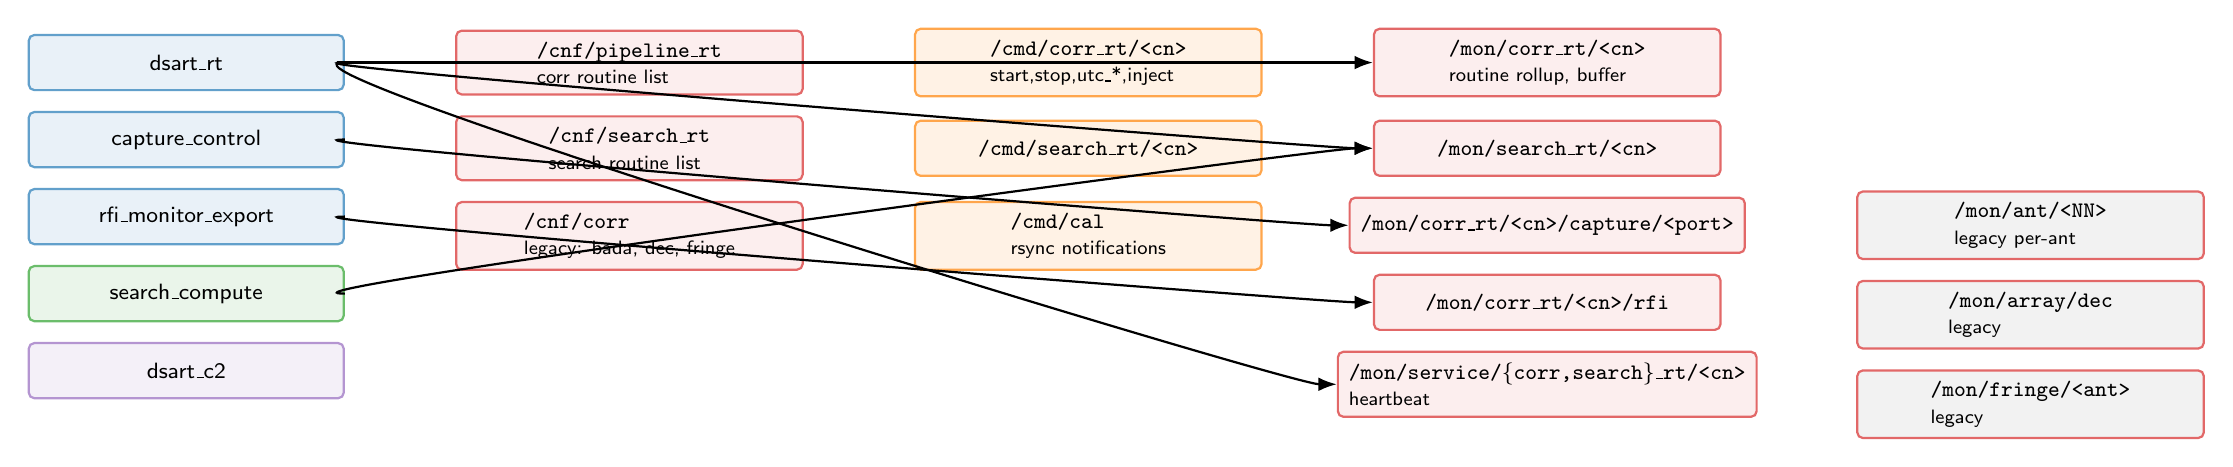
\begin{tikzpicture}[font=\sffamily\footnotesize,
   ns/.style={draw,rounded corners=2pt,fill=moncol!8,draw=moncol!70,
              minimum width=44mm,minimum height=7mm,align=left,inner sep=4pt},
   process/.style={draw,rounded corners=2pt,fill=corrcol!10,draw=corrcol!70,
              minimum width=40mm,minimum height=7mm,align=left,inner sep=4pt},
   sproc/.style={draw,rounded corners=2pt,fill=srchcol!10,draw=srchcol!70,
              minimum width=40mm,minimum height=7mm,align=left,inner sep=4pt},
   coproc/.style={draw,rounded corners=2pt,fill=coordcol!10,draw=coordcol!70,
              minimum width=40mm,minimum height=7mm,align=left,inner sep=4pt},
   thick,>=Latex,node distance=2.5mm,
]

% configuration namespaces
\node[ns] (cnf1) {\texttt{/cnf/pipeline\_rt}\\\scriptsize corr routine list};
\node[ns,below=of cnf1] (cnf2) {\texttt{/cnf/search\_rt}\\\scriptsize search routine list};
\node[ns,below=of cnf2] (cnf3) {\texttt{/cnf/corr}\\\scriptsize legacy: bada, dec, fringe};

% command namespaces
\node[ns,right=14mm of cnf1,fill=orange!10,draw=orange!70]
       (cmd1) {\texttt{/cmd/corr\_rt/<cn>}\\\scriptsize start,stop,utc\_*,inject};
\node[ns,right=14mm of cnf2,fill=orange!10,draw=orange!70]
       (cmd2) {\texttt{/cmd/search\_rt/<cn>}};
\node[ns,right=14mm of cnf3,fill=orange!10,draw=orange!70]
       (cmd3) {\texttt{/cmd/cal}\\\scriptsize rsync notifications};

% monitor namespaces
\node[ns,right=14mm of cmd1] (m1) {\texttt{/mon/corr\_rt/<cn>}\\\scriptsize routine rollup, buffer};
\node[ns,right=14mm of cmd2] (m2) {\texttt{/mon/search\_rt/<cn>}};
\node[ns,below=of m2] (m3) {\texttt{/mon/corr\_rt/<cn>/capture/<port>}};
\node[ns,below=of m3] (m4) {\texttt{/mon/corr\_rt/<cn>/rfi}};
\node[ns,below=of m4] (m5) {\texttt{/mon/service/\{corr,search\}\_rt/<cn>}\\\scriptsize heartbeat};

% legacy mon
\node[ns,right=14mm of m3,fill=gray!10] (m6) {\texttt{/mon/ant/<NN>}\\\scriptsize legacy per-ant};
\node[ns,below=of m6,fill=gray!10] (m7) {\texttt{/mon/array/dec}\\\scriptsize legacy};
\node[ns,below=of m7,fill=gray!10] (m8) {\texttt{/mon/fringe/<ant>}\\\scriptsize legacy};

% publishers (left)
\node[process,left=14mm of cnf1] (drt)   {dsart\_rt};
\node[process,below=of drt]      (cap)   {capture\_control};
\node[process,below=of cap]      (rfi)   {rfi\_monitor\_export};
\node[sproc,below=of rfi]        (sct)   {search\_compute};
\node[coproc,below=of sct]       (c2x)   {dsart\_c2};

% wires from process to mon keys (right side)
\draw[->] (drt)  .. controls +(6mm,0) and +(-6mm,0) .. (m1.west);
\draw[->] (drt)  .. controls +(6mm,0) and +(-6mm,0) .. (m2.west);
\draw[->] (drt)  .. controls +(6mm,0) and +(-6mm,0) .. (m5.west);
\draw[->] (cap)  .. controls +(6mm,0) and +(-6mm,0) .. (m3.west);
\draw[->] (rfi)  .. controls +(6mm,0) and +(-6mm,0) .. (m4.west);
\draw[->] (sct)  .. controls +(6mm,0) and +(-6mm,0) .. (m2.west);
% legacy publishers omitted for clarity
\end{tikzpicture}
}% end resizebox
\caption{etcd namespaces (red = monitor, orange = command, grey =
configuration) and their primary publishers.  Legacy keys (grey shaded)
remain populated through the M7 transition for downstream tooling that
hasn't been retargeted at the \texttt{\_rt} keyspace yet.}
\label{fig:control}
\end{figure}


\subsection{Per-block monitoring services}
\label{sec:mon-rfi}

Four monitoring services run alongside the data plane.

\paragraph{\texttt{capture\_control}} (per corr node, sidecar of
\codeword{dsart_capture}).  Publishes per-port packet counters,
arm state, and the per-block target specnum into
\codeword{/mon/corr_rt/<cn>/capture/<udp_port>} on a 2-s cadence.
Counters are cumulative; the InfluxDB pusher (below) differences
them and resets on \codeword{pid} flip.

\paragraph{\texttt{meridian\_fringestop} heartbeat} (per corr node,
internal to the casa38 wrapper at
\codeword{tools/ops/meridian_fringestop_rt.py}).
\begingroup\sloppy
A daemon thread publishes
\codeword{/mon/corr_rt/<cn>/meridian_ready} on a 10\,s cadence with
the fields \codeword{ready}, \codeword{pid}, \codeword{host},
\codeword{subband}, \codeword{dec_deg}, \codeword{ts_wall_unix},
\codeword{time_mjd}, \codeword{last_hdf5}, \codeword{n_hdf5}.
\codeword{n_hdf5} is the monotonic count of \codeword{*_sb<NN>.hdf5}
files in \codeword{--working-dir}, giving the dashboard a UVH5
production rate.  The wrapper is the only \codeword{bada} reader
and has no auto-restart, so the heartbeat is the sole way an
operator notices a meridian crash before \codeword{bada}
back-pressures and stalls \codeword{corr_fast}
(Section~\ref{sec:mfs}).\par\endgroup

\paragraph{\texttt{rfi\_monitor\_export}} (per corr node, sidecar of
\codeword{corr_fast_integration}).  \codeword{corr_fast} aggregates
16-cube RFI windows ($\approx 2.15$\,s) into a POSIX-shm ring at
\codeword{/dev/shm/dsart-rfi-window-<cn>}; each record has a
$4\times$ frequency-downsampled bandpass spectrum, the per-detector
flag fraction, and the per-antenna flag-fraction histogram.
\codeword{rfi_monitor_export} reads the shm ring and serves two
APIs:
\begin{itemize}[topsep=2pt,itemsep=2pt]
\item \codeword{/mon/corr_rt/<cn>/rfi} on etcd: scalar
      summaries (total flag fraction, bandpass-outlier flagged
      channel fraction, fraction of antennas flagged), per pol.
\item HTTP on port 5780: \codeword{/api/health},
      \codeword{/api/meta}, \codeword{/api/latest},
      \codeword{/api/recent?n=N}, returning the full RFI window
      records with base64-encoded numpy arrays.
\end{itemize}
The \codeword{dsa_monitor} dashboard on \codeword{h23} polls all
16 nodes' HTTP endpoints, backfills 30\,min on startup, and renders
the \emph{Antennas/RFI} tab.

\paragraph{\texttt{dsa\_monitor}} (\codeword{h23} user-systemd unit on
port 5778).  A Flask app that surfaces:
\begin{itemize}[topsep=2pt,itemsep=2pt]
\item A 12$\times$8 thumbnail grid of \emph{every} antenna's latest
      pre-flag bandpass (with HI~1.420\,GHz marked).
\item Per-antenna pre-flag bandpass spectrum, 30-min waterfall,
      flag-fraction spectrum, and 30-min flag waterfall.  XX and YY
      polarisations overlaid.
\item A per-antenna table joining the dashboard's RFI ring
      aggregates with the legacy \codeword{/mon/ant/<N>} etcd keys.
\item A \emph{SEFDs} tab that natively renders the calibrator-SEFD
      scanner's outputs (\codeword{state.json} + per-day PNG plot tree
      at \codeword{/media/ubuntu/ssd/vikram/sefd/sefd_dashboard/results/}),
      reached through the read-only seam
      \codeword{tools/dashboard/dsa_monitor/sefd_view.py} with three
      routes: \codeword{/sefds} (per-day $\times$ per-source grid with
      inline metrics + a heartbeat-driven scanner-freshness pill),
      \codeword{/sefds/source/<src>} (per-calibrator comparison: metrics
      table + diagnostic plots), and \codeword{/sefds/day/<date>}
      (per-day detail).  Plot files are served back through
      \codeword{/sefds/results/<path>} with a path-traversal guard.  The
      scanner itself still runs in \codeword{sefd_dashboard.service}
      (casa38 conda env) --- now retargeted at
      \codeword{sefd_scanner.py} which spawns the
      \codeword{scanner_loop} from the new \codeword{scanner.py} module
      \emph{without} a Flask app, so port 5777 is retired --- and
      writes a \codeword{scanner_heartbeat} sidecar file on every poll
      cycle, so the dashboard's liveness pill stays green on quiet
      nights when \codeword{state.json} itself doesn't change.  The
      legacy \codeword{sefd_dashboard/app.py} is kept as a
      back-compat shim that re-exports the scanner helpers (so
      external scripts importing \codeword{from app import load_state}
      keep working) and, if invoked directly, prints a deprecation
      warning before serving the old port-5777 UI.
\item A C2-aware \emph{Burst candidates} tab.
\item A \emph{Control} tab.  This started in Phase~8 with the four
      bring-up verbs (\codeword{start} / \codeword{stop} /
      \codeword{utc_start} / \codeword{utc_stop}) and has been
      extended through M7.6 with: an arm-and-shoot \emph{voltage
      injection} form (\codeword{POST /control/inject},
      Section~\ref{sec:inject-arm}); a \emph{calibration probe}
      (\codeword{/control/inject_calibrate}) that drives the
      bootstrap S/N calibration loop and writes
      \codeword{/cnf/inject/snr_calibration/<bucket>}; a
      \emph{Dump Now} button (\codeword{/control/dump_now}) that
      synthesises a manual \codeword{C2TriggerPacket} keyed off the
      live search-cube ring; a \emph{C2 dumps gate}
      (\codeword{/control/dumps_enabled}, GET/POST) that flips the
      runtime kill-switch read by \codeword{coincidencer.DumpsGate};
      fleet-recovery operations \codeword{update_dsart} (git
      fetch + ff-merge or reset on every node, with progress
      streamed back), \codeword{restart_all}, and
      \codeword{restart_c2}; and --- after the 2026-06-01 swap
      (commit \codeword{cb1bdcf}) --- a
      \emph{Delete SNR calibration} button (\codeword{/control/delete_snr_cal},
      \codeword{inject_calibration.delete_snr_calibrations}) that
      clears the per-(DM, width) bootstrap fluence$\to$SNR $K$ table
      at \codeword{/cnf/inject/snr_calibration/<bucket>} so the
      operator can re-measure the relation.  The previous
      \emph{Delete K-cal (beamformer weights)} fan-out
      (\codeword{fleet_kcal.delete_kcal_fleet}) was a footgun ---
      a single dashboard click could wipe every corr node's
      beamformer-weights table --- so it was retired from the UI;
      \codeword{fleet_kcal.py} is retained for CLI use.  Every verb
      writes \codeword{/mon/audit/control/<iso-ts>} regardless of
      outcome.  A 2026-06-02 restructure (i) added a sticky
      table-of-contents jump-nav at the top of the Control tab; (ii)
      folded the standalone \emph{Restart all} and \emph{Update
      dsa110-rt} panels into the \emph{Verbs} panel and the
      \emph{Recent C2 activity} list into the \emph{C2 recovery \&
      activity} panel so the operator's eye sweeps top-down through a
      single column; and (iii) retired the now-redundant
      \codeword{bounce_search} verb (the C2 stall defenses landed the
      same day made it unnecessary).  Pressing \emph{Start fleet} now
      runs the start-time housekeeping fanout described in
      Section~\ref{sec:bringup-cleanup} \emph{before} broadcasting the
      \codeword{start} verb to etcd, and the per-host cleanup summary
      is attached to the verb's JSON response under
      \codeword{node_cleanup}.
\item The 5-state lifecycle banner described in
      Section~\ref{sec:bringup-banner}, rolled up by
      \codeword{/control/system_state} from the
      \codeword{corr_fast_ready} keys, the orchestrator
      \codeword{routines.<name>.pid} fields, and the per-port
      \codeword{capture/<port>.arm_state}; it is the
      operator's single ``safe to arm'' signal.
\end{itemize}
Antenna labels are sourced from
\codeword{configs/corr_setup_96.yaml::antenna_order} so the
operator sees real DSA antenna numbers, not 0-based cube indices.


\subsection{InfluxDB pusher and Grafana}

A separate sub-agent contributed the etcd $\rightarrow$ InfluxDB
pusher (\codeword{tools/dashboard/dsart_rt_to_influx/}).  It runs
as a system-systemd unit on \codeword{lxd110h20} (co-located with
the long-running \codeword{influxd 1.7} so writes go loopback),
polling the etcd prefixes
\codeword{/mon/{corr_rt,search_rt,service/*,c2/}/} every 1\,s,
dedup'd on \codeword{mod_revision}.  As of 2026-05-30 the pusher
writes \textbf{twelve} measurements into the \codeword{dsa110} InfluxDB
database: \codeword{corr_rt_routine}, \codeword{corr_rt_buffer},
\codeword{corr_rt_capture}, \codeword{corr_rt_rfi},
\codeword{corr_rt_corr_fast} (per-block service-start epoch from
\codeword{/mon/corr_rt/<chgroup>/corr_fast}),
\codeword{corr_rt_meridian} (the meridian-fringestop liveness
sub-dict from \codeword{/mon/corr_rt/<cn>/meridian_ready}: fields
\codeword{ready}, \codeword{n_hdf5}, \codeword{pid},
\codeword{dec_deg}, \codeword{age_s}; tagged \codeword{cn_id},
\codeword{host}, \codeword{subband}; routed \emph{before} the bare-CN
rollup so the per-key sub-paths are picked up correctly),
\codeword{corr_rt_heartbeat}, \codeword{search_rt_routine},
\codeword{search_rt_compute} (M7.6 C1$\to$C2 metering rollup from
\codeword{/mon/search_rt/<cn>/compute/<half>}),
\codeword{search_rt_heartbeat}, \codeword{c2_service} +
\codeword{c2_receiver} (top-level + RX counters from
\codeword{/mon/c2/h23}), and \codeword{c2_inject_match} (the
\codeword{inject_match} sub-dict from the same key).  Cumulative
capture counters are emitted as both the raw counter and a
pre-differenced \codeword{*_delta} field; the delta state is keyed
on \codeword{(cn_id, udp_port)} and reset on \codeword{pid} flip or
any non-monotonic dip, so the time series never shows a negative
spike.  \codeword{schema_version} mismatches log loud and refuse to
ingest, preventing silent drift between publisher and consumer.

The companion Grafana dashboard \codeword{dsartRtMpV1} runs on
\codeword{lxd110h20:3000}.  Its 89 panels (rebuilt 2026-05-30 to add
the \emph{Meridian fringestop} row + four panels: ready-node fleet
sum --- target 16; heartbeat freshness per cn with a crit threshold
at $>$60\,s; UVH5 output rate per cn; snapped imaging dec per cn)
are organised into 15 labelled rows (fleet at-a-glance, service
heartbeats, routine state, capture pipeline, capture integrity, cube
cadence, PSRDADA buffer health, RFI flagger, meridian fringestop, C1
batch receiver, C1$\to$C2 candidate flow, C2 trigger pipeline, last
C2 trigger, C2 housekeeping, voltage-injection match) and
self-document the deploy-skew root cause of any silent panels (the
\emph{PSRDADA buffer health} row includes the
\codeword{update_dsart}/\codeword{stop}/\codeword{start}
remediation steps inline; the C1$\to$C2 row distinguishes
\codeword{batches_ok/s} including heartbeats from \codeword{rows_in/s}
candidate-bearing rows so a quiet sky reads as healthy not broken;
all eight rate panels are labelled \codeword{ops/s} per operator
preference, switched 2026-05-30 from Grafana's \codeword{cps}).
The dashboard is built by an idempotent generator
(\codeword{tools/dashboard/dsart_rt_to_influx/grafana/build_dashboard.py})
so the JSON snapshot under version control is exactly what's live;
re-POST is one command and overwrites in place at the pinned UID.

Catalogue of every M7.6 service: \codeword{docs/m7/M7.6-SERVICES.md}.
Per-key schemas: \codeword{docs/m7/M7.6-MONITOR-POINTS.md} and
\codeword{docs/m7/M7.6-MONITOR-POINTS-SEARCH.md}.


% =============================================================================
\section{Development pathway}
\label{sec:devpath}

\subsection{Where the project has been}

\codeword{dsa110-rt} has been built up in phased milestones, each
gated on a deterministic set of acceptance benches against the
legacy contract (\codeword{REALTIME_FRB_SEARCH.md}) and the
revamp plan (\codeword{dsa110-rt_revamp_*.plan.md}).

\begin{itemize}[topsep=2pt,itemsep=2pt]
\item \textbf{M0--M1}: repo skeleton, conda env, frozen numerical
      contracts, \codeword{build_dm_plan.py} produces
      \codeword{configs/dm_plan.npz}.
\item \textbf{M2}: \codeword{corr_slow_compute}, fringe-stop cache,
      UVH5 smoke against the legacy schema.
\item \textbf{M3}: full \codeword{corr_fast_compute} on one chgroup,
      end-to-end RFI + cal + GEMM + grid + DM.
\item \textbf{M4a}: corr-side UDP transport, sparse pattern, on-host
      loopback bench.
\item \textbf{M4b}: real 40\,GbE pair-rate; 16$\rightarrow$4
      corner-turn.  Passed 2026-05-15.
\item \textbf{M5}: \codeword{search_rx} + \codeword{search_compute};
      $\ge 8$ cubes/s sustained, p99 $\le 134$\,ms.
\item \textbf{M6}: cube ring, dump-on-trigger, cluster logger (legacy
      DBSCAN, since stripped in favour of C2).
\item \textbf{M7.0--M7.1}: \codeword{dsart_rt} skeleton, real-time
      gate.
\item \textbf{M7.2--M7.3}: production fan-out 16$\rightarrow$4
      search nodes, RFI ON, real SNAP, full operating point.
\item \textbf{M7.4}: C1/C2 coincidencer, fleet-wide gate.  PASSED
      2026-05-28.
\item \textbf{M7.4 Phase~8 (cold-start triad, 2026-05-28/29)}:
      kernel JIT warmup before the corr-side ready-sentinel (fixes
      fada cold-start packet-loss); unconditional 0-row C1$\to$C2
      heartbeats every 20\,s + C2 \codeword{startup_grace_s}
      (180\,s) + per-cube event-loop yield (fixes the C1$\to$C2 7/8
      stuck-connections cascade); voltage injection moved post-cal
      (so the injected source's per-antenna fringe is in the
      calibrated array frame); \codeword{dada_dbmetric} parsing fix
      and Grafana buffer panels; trigger-criteria tightening.
\item \textbf{M7.4.1--M7.4.2 (May 27)}: GPU-side scatter
      ($12.3\times$ speedup, byte-identical to CPU dense path);
      Layer-1 coverage correction kills $\sim\!50000\times$ of the
      synth-Gaussian false alarms on the stage-2-absent search path.
\item \textbf{M7.5--M7.6}: RFI tuning + monitoring infrastructure
      (\codeword{rfi_monitor_export}, \codeword{dsa_monitor},
      InfluxDB pusher, Grafana); 5-state lifecycle banner
      (Section~\ref{sec:bringup-banner}); fleet-recovery operations
      from the dashboard's Control tab; C1$\to$C2 metering (width
      cap + per-block cap) with a per-half rollup published to
      \codeword{/mon/search_rt/<cn>/compute/<half>}; cube ring
      deepened to 24 slots (subsequently shrunk to 16 in the
      2026-05-31 memory-budget audit when the prior $3.2$\,GiB/slot
      arithmetic was found to be 4$\times$ wrong); real-time
      freshness re-seek; DM offset fix in the stage-2-absent escape
      hatch; NE2001 galactic-DM classifier as the sole bright-class
      discriminant; meridian\_fringestop integrated as the sole
      bada reader (2026-05-30, Phase 9); the C1$\to$C2 stall fix
      (2026-05-30: process-pool plotter, rolling-window dump-rate
      cap, demotion of \codeword{bright_pulsar}/\codeword{bright_galactic}
      to \codeword{log_only}); the DM-smear floor and noise-color
      SNR de-rating defenses (2026-05-30 / 2026-06-02); the search
      MJD clock fix (2026-06-01); and the slow-vis UVH5 time-anchor
      bridge (2026-06-02).
\item \textbf{M7.7 (2026-06-02--10, real-time + correctness
      campaign)}: Option~A coarse-DM consolidation onto the corr
      side with the F34 2-block sliding window;
      symmetric-shift padding for 100\,\% fine-DM coverage;
      production DM plan v2 ($N_\mathrm{fine}=272$, $\theta=1.6$,
      DM 100--2653); \codeword{StaticSkyMean} replacing the EMA
      static-sky subtractor; the big-block op-point
      ($T_\mathrm{det}=256$, cadence 192) with the fftshift fold and
      the rfft imager --- a search half now sustains
      $\sim$166\,ms/cube against the 201.3\,ms budget
      ($\sim$17\,\% headroom); Layer-2 $\sigma_k$ clamp (T1) +
      escape hatch; detector input clip (fp16 overflow hardening);
      the wing-decode fix (dynamic \codeword{n_kernel_max_t},
      closing a periodic 64-sample scoring blind spot);
      candidate sky-coordinate fixes (centred layout, axis
      transposition, exact \codeword{cell_lambda} pixel scale);
      the injection-system overhaul ($\sqrt{\text{flux}}$ voltage
      convention, linear $K$ model, width-independent per-DM-band
      calibration, specnum proximity gate + wall-clock fallback,
      saturation guard + descending ladder + position rotation,
      32-block auto-arm margin with staleness extrapolation); the
      T1--T8 robustness series (runtime-watch counters,
      \codeword{CalProbeShadow} metering bypass,
      \codeword{HealthSnapshot} pre-flight, bounded cube uploads,
      C2 startup-grace pre-expiry); dumps-gated event directories;
      and the C2 stacked-waterfall plotter.
\end{itemize}

\subsection{What is still pending}

The M7.4 Phase plan (\codeword{docs/M7.4_PHASE_PLAN.md}) tracks the
outstanding items.  As of 2026-06-10 the remaining work is:

\begin{enumerate}[topsep=2pt,itemsep=2pt]
\item \textbf{Phase 6c characterisation}: the 2026-06-08--10
      campaign delivered most of this --- fluence linearity
      ($K$ constant to $\pm 4\%$ over $3.5\times$), width
      independence ($w\in\{2,4,8,16\}$), a 12-point cadence phase
      sweep (11/12 apex recovery post-wing-fix), four-quadrant
      position recovery to within a pixel, and per-DM-band $K$
      values across DM 150--2500.  Still open: RFI-zero-fill
      quantification of the total-power bias when the flagger zeros
      a fraction $f$ of cells in the same block as a burst, and a
      systematic DM-recovery bias study against the v2 plan.
\item \textbf{Slow-vis archive replay}: re-derive a sample of the
      legacy \codeword{calibration23} K-cal tables from the post-2026-05-30
      UVH5 archive (now anchored on correct timestamps; see
      Section~\ref{sec:mfs}) and cross-check the resulting per-corr
      \codeword{antennas.out} blobs against the production fast-corr
      \codeword{--apply-cal} input.  Pre-existing UVH5 files written
      before commit \codeword{e6ee7cd} carry the stale anchor and
      need to be either backfilled (rewrite \codeword{time_array} in
      each HDF5 from the file mtime, see
      \codeword{tools/inspect_uvh5.py}) or excluded.
\item \textbf{Control verbs}: implement the remaining
      \codeword{prepare}, \codeword{record}, \codeword{inject}
      (orchestrator-side; the corr-side \codeword{inject} watcher is
      already wired),
      \codeword{reload_cal}, \codeword{reload_flagants},
      \codeword{ctrltrigger}, \codeword{trigger} verbs and migrate
      consumers off the legacy \codeword{/mon/corr/<n>} keyspace.
\item \textbf{Detector v2}: the v1 deterministic detector is in
      production with the 2026-05-30 / 2026-06-02 DM-smear floor
      and noise-color de-rating defenses (Section~\ref{sec:c1});
      the v2 upgrade pathway is the subject of~\Cref{sec:c1path}.
\end{enumerate}


% =============================================================================
\section{Monte-Carlo S/N loss as a function of DM}
\label{sec:mcloss}

\subsection{Model}

The production DM plan is
\codeword{dm_plan_N8_dmmin100_tol1.6_v2.npz}:
$N_\mathrm{fine}=272$, $N_\mathrm{coarse}=8$, $\DM_\mathrm{min}=100$,
$\DM_\mathrm{max}=2653$\,pc\,cm$^{-3}$, and Levin tolerance
$\theta=1.6$.  Adjacent fine-DM trial spacings sit in
$[9.34,\,9.58]$\,pc\,cm$^{-3}$ across the whole range, essentially
uniform.

Consider a delta-function FRB at intrinsic DM $\DM_\mathrm{true}$.
At the search-time matched filter, two mechanisms broaden the
observed pulse:

\textbf{(a) Intra-channel dispersion smearing} at the bottom of the
processed band (the worst-case channel, since $\partial\tau/\partial\nu
\propto 1/\nu^3$):
\begin{equation}
   w_\mathrm{chan}(\DM_\mathrm{true}) =
       \big|\partial\tau/\partial\nu\big| \cdot \dnu
     = \frac{2\,\Kdm \cdot \DM_\mathrm{true} \cdot \dnu}{\nubot^{3}}.
   \label{eq:wchan}
\end{equation}
The relevant $\dnu$ is the channel width \emph{at the point of
incoherent dedispersion}.  In the M7.3+ production geometry that is
the chan-sum-8 channel width
$\dnu^\mathrm{prod} = 244.140\,$kHz; in the v1 / native geometry it
is $\dnu^\mathrm{nat} = 30.518\,$kHz.

\textbf{(b) Inter-channel dispersion smearing} from the residual DM
mismatch $\Delta\DM = |\DM_\mathrm{true} - \DM_\mathrm{trial}^\star|$
where $\DM_\mathrm{trial}^\star$ is the closest fine-DM trial:
\begin{equation}
   w_{\Delta\DM}(\Delta\DM) =
       \Kdm \cdot \Delta\DM \cdot \Big(\tfrac{1}{\nubot^2} - \tfrac{1}{\nutop^2}\Big).
   \label{eq:wmiss}
\end{equation}
This is the smear across the \emph{full} processed band introduced by
incoherently dedispersing at the wrong DM.  At
$\Delta\DM = 1\,$pc\,cm$^{-3}$ it is $\sim 0.57$\,ms; at the worst
case $|\Delta\DM|=\Delta\DM_\mathrm{spacing}/2 \approx
4.7$\,pc\,cm$^{-3}$ it is $\sim 2.6$\,ms.

The two add in quadrature.  The user-supplied formulae for the
\emph{measured} and \emph{ideal} (perfectly matched DM) widths are
\begin{equation}
   w_\mathrm{ideal}  = w_\mathrm{chan}(\DM_\mathrm{true}),
   \qquad
   w_\mathrm{meas} = \sqrt{w_\mathrm{chan}^2 + w_{\Delta\DM}^2}.
   \label{eq:widths}
\end{equation}
For an idealised matched filter on a top-hat-broadened delta in white
noise the S/N scales as $w^{-1/2}$, hence the S/N loss factor is
\begin{equation}
   \eta = \frac{\mathrm{S/N}_\mathrm{meas}}{\mathrm{S/N}_\mathrm{ideal}}
        = \sqrt{w_\mathrm{ideal}/w_\mathrm{meas}}.
   \label{eq:eta}
\end{equation}
We report the loss as both $\Delta\mathrm{SNR}_\mathrm{dB} = 10\log_{10}\eta$
and a per-cent loss $1-\eta$.

The DM-plan Levin tolerance $\theta=1.6$ implies a design-target loss
of $\Delta\mathrm{SNR}_\mathrm{dB} = 10\log_{10}(1/\theta) = -2.04$\,dB
$\approx 37\,\%$ S/N loss in the limit where channel smearing
\emph{equals} DM-mismatch smearing at the spacing midpoint.

\subsection{Monte-Carlo procedure}

We draw $N=2\times 10^5$ values of $\DM_\mathrm{true}$ uniformly on
$[100, 2653]$\,pc\,cm$^{-3}$, look up the closest fine-DM trial via a
nearest-neighbour search on the plan's \codeword{fine_dm} array,
compute the two widths from \Cref{eq:wchan,eq:wmiss}, and form $\eta$
from \Cref{eq:eta}.  We do this twice: once with the native channel
width $\dnu^\mathrm{nat} = 30.518$\,kHz, once with the chan-sum-8
channel width $\dnu^\mathrm{prod} = 244.140$\,kHz.  The simulation
script is at \codeword{tools/sim/dm_plan_snr_loss.py} and is
seeded for reproducibility.

\subsection{Results}

\Cref{fig:mcloss} shows the result; the per-percentile summary is in
\Cref{tab:mcloss}.  Two features dominate:

\begin{itemize}[topsep=2pt,itemsep=2pt]
\item The fine-DM plan spacing is essentially uniform across the full
      DM range, so the $|\Delta\DM|$ distribution is uniform on $[0,
      \,\Delta\DM_\mathrm{spacing}/2]$ with $\Delta\DM_\mathrm{spacing}\sim 9.4$\,pc\,cm$^{-3}$
      (median $|\Delta\DM| = 2.36$, p99 $= 4.66$\,pc\,cm$^{-3}$).
\item Because $w_\mathrm{chan} \propto \DM$ but $w_{\Delta\DM}$ is
      independent of $\DM$, the loss is \emph{largest at the low end
      of the searched range} (where channel smearing is smallest so
      any mismatch dominates) and falls toward a floor at high DM.
      Starting the plan at $\DM_\mathrm{min}=100$ deliberately cuts
      off the catastrophic $\DM\lesssim 50$ tail that a 0-based plan
      suffers.
\end{itemize}

In the production geometry (chan-sum 8, $\dnu = 244$\,kHz) the
median S/N loss is \textbf{17.6\,\%} ($-0.84$\,dB), the
worst-10-per-cent loss is \textbf{51.9\,\%} ($-3.18$\,dB), and the
worst-1-per-cent reaches $\sim 74\,\%$ ($-5.8$\,dB).  The median is
comfortably inside the $\theta=1.6$ design target of $-2.04$\,dB;
the tails reflect the coarser v2 trial spacing, accepted in exchange
for the $2.5\times$ smaller per-GPU trial count that funds the
real-time budget.

In the native geometry (chan-sum 1, $\dnu = 30.5$\,kHz, used only
during early commissioning / detector-bench replays) the median loss
is \textbf{66.1\,\%} ($-4.70$\,dB).  This is far worse than the design
target and is the direct quantitative justification for the corr-side
$8\times$ channel sum: the channel sum buys $\sqrt{8}\!\sim\!2.8\,$dB
of headroom across the DM range simply by increasing
$w_\mathrm{chan}$ until it dominates the matched-filter width.

\begin{figure}[ht]
\centering
\includegraphics[width=0.98\linewidth]{figs/dm_plan_snr_loss.pdf}
\caption{Monte-Carlo S/N-loss summary against the production v2 DM
plan, $N=2\!\times\!10^5$ draws of $\DM_\mathrm{true}$ uniform on
$[100, 2653]$\,pc\,cm$^{-3}$.
\textbf{(a)} Fine-DM trial spacing as a function of $\DM_\mathrm{trial}$.
\textbf{(b)} Resulting $|\Delta\DM|$ distribution to the nearest
trial; native and chan-sum-8 are identical because the trial grid is
the same.
\textbf{(c)} Per-DM intra-channel smearing $w_\mathrm{chan}$ and
DM-mismatch smearing $w_{\Delta\DM}$ in the production (chan-sum 8)
geometry; the dotted horizontal line marks the search sample period.
\textbf{(d, e)} S/N loss in dB and per cent, per-bin median (solid)
$\pm$ 16/84 spread (shading) and worst-1\,\% tail (dashed); native
$\dnu$ in green, production $\dnu$ in red.  The grey dotted line in (d)
is the $\theta=1.6$ Levin design target ($-2.04$\,dB).
\textbf{(f)} Text summary.}
\label{fig:mcloss}
\end{figure}

\begin{table}[ht]
\centering
\caption{Monte-Carlo S/N loss against the production v2 DM plan
($N_\mathrm{fine}=272$, $\theta=1.6$, $\DM_\mathrm{min}=100$,
$\DM_\mathrm{max}=2653$\,pc\,cm$^{-3}$).  The ``worst'' columns are the
$10\,\%$ and $1\,\%$ tails (most negative dB, largest per-cent).}
\label{tab:mcloss}
\small
\begin{tabular}{lrrr}
\toprule
Geometry           & median           & worst 10\,\%     & worst 1\,\% \\
\midrule
\multicolumn{4}{l}{\emph{Loss (dB)}} \\
~~native, $\dnu = 30.5$\,kHz        & $-4.70$          & $-7.63$          & $-10.31$    \\
~~production, $\dnu = 244$\,kHz     & $-0.84$          & $-3.18$          & $-5.80$     \\
\midrule
\multicolumn{4}{l}{\emph{Loss (per cent)}} \\
~~native, $\dnu = 30.5$\,kHz        & $66.12\,\%$      & $82.76\,\%$      & $90.70\,\%$ \\
~~production, $\dnu = 244$\,kHz     & $17.61\,\%$      & $51.88\,\%$      & $73.71\,\%$ \\
\bottomrule
\end{tabular}
\end{table}

\subsection{Caveats}

The model deliberately follows the user's stated formula
(quadrature sum of channel and DM-mismatch smearing) and omits:

\begin{itemize}[topsep=2pt,itemsep=2pt]
\item Scattering and intrinsic burst width: real FRBs are not delta
      functions.  Adding a scattering tail $w_\mathrm{sc} \propto
      \nu^{-4}$ at the bottom of the band would push the
      ``ideal-versus-measured'' ratio toward unity at low DM (since
      $w_\mathrm{chan}$ is no longer the smallest contribution).
\item The matched-filter floor at one $t_\mathrm{int}^\mathrm{search}$
      sample ($\approx 1049\,\mu$s).  Below that the boxcar bank
      cannot resolve a narrower pulse anyway, so $w_\mathrm{chan} <
      t_\mathrm{int}^\mathrm{search}$ does not buy any additional
      S/N; $w_\mathrm{ideal}$ should be replaced by
      $\max(w_\mathrm{chan}, t_\mathrm{int}^\mathrm{search})$ if
      one wants the absolute matched-filter S/N rather than the
      relative loss --- this materially softens the reported
      low-DM tail, since at $\DM \lesssim 800$ the channel smearing
      is below the sample period anyway.
\item The boxcar bank is discrete
      (\codeword{K_time}$\in\{1,2,\dots,64\}$).  The closest matched
      filter to a given width incurs an additional discretisation
      loss of a few per cent on top of the dispersion-only loss
      reported here.
\item Pulse-profile and finite-bandwidth coherence effects (these
      are negligible at DSA-110's 187\,MHz band for incoherent
      dedispersion).
\end{itemize}


% =============================================================================
\section{Development pathway for adding intelligence to the C1 detector}
\label{sec:c1path}
\label{sec:c1v2}

The v1 deterministic detector (\Cref{sec:c1}) is intentionally
\emph{boring}: a separable conv-bank fed by an analytically
Gaussian-equivalent noise model.  This is the right starting point
for an on-sky pipeline because every false-positive rate and every
real-time budget is calculable from first principles.  However, the
revamp plan (\codeword{dsa110-rt_revamp_*.plan.md} §4.4) and the
critical review (\codeword{dsa110-rt_critical_review.md} §6) both
note that the detector interface is \emph{deliberately} v1-locked
only at its \codeword{forward()} signature: the internal architecture
and state-dict layout are explicitly free to change at v2.  The
\codeword{Detector} Python \codeword{Protocol} and the
\codeword{TriggerCondition} chain are exactly the seams for that
upgrade.

This section expands on the possibilities discussed in the revamp
MD and proposes a concrete, phased upgrade plan.

\subsection{Phase~I: PSF-matched image kernels}

In v1, all four $K_\mathrm{img}$ kernels (\codeword{unit},
\codeword{psf}, \codeword{psf_shift_lm}, \codeword{psf_shift_l})
ship as the trivial $1\times 1$ delta (the \codeword{D10}
placeholder in \codeword{M5_PLAN_FIXES.md}).  This is correct for
the cube-injection bench because that bench operates on the
already-imaged cube where the PSF has already been convolved into
the noise structure.  For on-sky data the analogous statement is
that the noise in $I(l, m)$ is correlated by the dirty-beam pattern
$B(l, m)$ over a length scale set by the array configuration.

A drop-in v1.5 would replace the deltas with the PSF and its
half-pixel-shifted variants, L2-normalised:
\begin{equation}
   K_\mathrm{img}^{(\mathrm{psf})}(\Delta l, \Delta m) =
        \frac{B(\Delta l, \Delta m)}{\sqrt{\sum_{\Delta l, \Delta m} B(\Delta l, \Delta m)^2}},
   \label{eq:psfkern}
\end{equation}
with the half-pixel shifts taking out the dirty-beam side-lobe
ringing.  The DSA-core cross-shaped PSF guarantees a real burst
leaves twin survivors at small $\Delta l$ or $\Delta m$ (one along
each arm), which is exactly the \emph{OR}-semantics the C1 merger
already encodes (\Cref{sec:c1}).  The PSF kernels would re-weight
those survivors before NMS, recovering an additional $\sim 1$\,dB at
fixed false-positive rate.  \emph{Risk}: doubles the conv-bank FLOPs.
\emph{Gate}: the M5 cube-injection bench remains the FAR yardstick,
with a single new bench against a pre-imager (sparse-COO) cube to
exercise the matched filter explicitly.

\subsection{Phase~II: PSF-aware (l, m) merger geometry}

The C1 merger's $\mathrm{lm\_cells}$ radius is currently a flat
constant.  In phase~II it would scale with the local PSF synthesized
beam size, which is itself a function of $|u_\lambda|, |v_\lambda|$
distribution at the trial frequency.  Operationally this is a
single-call lookup against a per-(l, m) precomputed beam-size table
in the same \codeword{MergerConfig}; the geometry stays $O(N^2)$ in
the survivor list and the table is built at \codeword{prepare} time
when the (u, v) sparsity pattern is sealed.

\subsection{Phase~III: TriggerCondition extensions}

The C1 emit path already runs each surviving candidate through a
\codeword{TriggerCondition} predicate chain.  Two named conditions
listed in the revamp MD §4.4 as ``commented future yaml entries''
are immediate low-risk wins:

\begin{itemize}[topsep=2pt,itemsep=2pt]
\item \codeword{PointingExclusion}: cull candidates whose $(l, m)$
      falls within a pointing-defined exclusion set (the Sun, the
      Moon, known continuum sources).  Input is a \codeword{bad_lm_csv}
      pointing file rotated against $\delta_0$ at \codeword{prepare}
      time.  Zero compute cost at run time (one bilinear lookup per
      candidate).
\item \codeword{LearnedClassifier}: a small CNN or gradient-boosted
      classifier consuming a fixed-size window around each survivor
      (e.g.\ a $32\!\times\!32\!\times\!8$ patch in $l, m, t$ at the
      survivor's $f_\mathrm{dm}$).  This is the smallest possible
      ``ML triage'' surface --- no inference on the full cube,
      just a fixed-cost score per candidate, of which there are
      typically $\le$ a few hundred per cube before the merger.
      Cost-per-candidate inference at fp16 on the host GPU is
      $\mathcal{O}(10^4)$ MACs, far below any pacing budget.
\end{itemize}

The model can be trained offline against a labelled corpus generated
by (i) the M6 cube-injection bench (truth-positive pulses with known
$\DM, l, m, w$) and (ii) the M7.4 dump archive (truth-positive bursts
plus operator-vetted RFI examples).

\subsection{Phase~IV: a learned detector v2}

Phases I--III preserve the deterministic conv-bank as the
\emph{detection} surface and add learned filters only after the
fact.  Phase~IV replaces the conv-bank itself with a learned
detector, drop-in at the \codeword{Detector} Protocol.  Three
architectures are realistic on the 2080 Ti budget (the revamp MD §4.4
explicitly reserves INT8 Tensor-Core capacity for this):

\begin{enumerate}[topsep=2pt,itemsep=2pt,leftmargin=*]
\item \textbf{2-D image-domain CNN per fine-DM trial}.  A small
      VGG-style encoder runs once per cube per fine-DM trial,
      emitting a $(l, m, t)$ heatmap which is then NMS'd by the
      same decoder as the v1 conv-bank.  Direct cost: $K_\mathrm{img}
      = 1$ but the encoder amortises the work across many time
      steps.
\item \textbf{(l, m, t) 3-D CNN with a (DM, t) recurrence}.  The
      $f_\mathrm{dm}$ axis is folded into the channel dimension; an
      LSTM or temporal-conv head replaces the running boxcar.
      Captures the dispersion ramp explicitly, which the v1 boxcars
      cannot (they are blind to slope).
\item \textbf{Spectrogram-style Transformer} on the dedispersed
      $(l, m, f_\mathrm{dm}, t)$ tensor.  Costlier; only viable if
      the FLOPs budget can be moved to INT8 / sparse attention.
\end{enumerate}

The revamp MD's explicit guidance is to keep \emph{shadow A/B} as the
rollout mechanism: v2 runs alongside v1 on the same cube, emits its
own C1 batch with a distinct \codeword{kernel_id} namespace, and C2
clusters both outputs into the same time window.  Operator-level
control via \codeword{c1.detector_mode = {v1, v2, both}} comes
for free from the Protocol interface.

\subsection{Phase~V: dedispersion-domain RFI features}

Three RFI-class signals that the v1 detector cannot suppress
analytically but a learned model could:

\begin{enumerate}[topsep=2pt,itemsep=2pt,leftmargin=*]
\item \textbf{DM-blind broadband RFI}.  A swept-frequency interferer
      leaves a track that is constant in $\DM$ (a vertical line in
      a $\DM\!-\!t$ waterfall).  v1's $K_\mathrm{dm}$ boxcars
      \emph{integrate} over this track and inflate the score; a
      Layer-3 per-fine-DM EMA (deferred in v1) would catch it,
      but a learned model can do the same with no additional state.
\item \textbf{Position-domain RFI clusters}.  Some interferers leave
      a stable image-plane footprint at the position of a known bright
      continuum source's PSF side-lobes.  \codeword{PointingExclusion}
      catches the obvious ones; a learned feature on the local
      image-plane pattern catches the rest.
\item \textbf{Per-baseline weight learning}.  The cal-apply step
      already multiplies each $E_i^p(\nu, t)$ by a complex gain;
      the residual visibility weights that should go into the
      X-engine GEMM are currently uniform across baselines.  A
      learned per-baseline weight (a single scalar per
      $(i, j, \nu_\mathrm{cg})$) would damp the contribution of
      baselines that are systematically RFI-prone, at zero extra
      online inference cost (the weight table is rebuilt offline).
\end{enumerate}

\subsection{Phase~VI: multi-pulse and DM--position joint priors}

A real-time repeater whose source position is approximately known
(e.g.\ from a previous detection) can have its expected $(l, m, \DM)$
window encoded as a prior in C2 trigger-criteria, rather than in C1.
At C2 the prior is one extra \codeword{require:} block in
\codeword{c2_trigger_criteria.yaml}; at C1 the same prior can be
used to \emph{lower} \codeword{c1.snr_min} only for candidates
falling inside the prior window, recovering an additional $\sim 0.5$
to $1.0$\,$\sigma$ of sensitivity to known-position repeaters.

\subsection{Suggested order, gating and risks}

\Cref{tab:c1pathway} summarises the proposed pathway.  Phases~I--III
are low-risk drop-ins that can ship in parallel; Phase~IV is the only
phase that breaks the deterministic-FAR guarantee and therefore needs
a full shadow A/B period before becoming the default.

\begin{table}[ht]
\centering
\caption{Proposed C1 intelligence upgrade pathway.  ``Surface''
denotes the data the new component consumes; ``FAR'' indicates
whether the change preserves the v1 analytical false-positive
rate.}
\label{tab:c1pathway}
\small
\begin{tabular}{p{2.2cm}p{4cm}p{2.0cm}p{2.6cm}p{2.6cm}}
\toprule
Phase & Change & Risk & FAR preserved & Gate \\
\midrule
I  & PSF-matched image kernels & low & yes & M5 cube-inject bench \\
II & PSF-aware merger lm radius & low & yes (merger geometry only) & M5 bench + replay \\
III a & \codeword{PointingExclusion} & low & yes & operator vet \\
III b & \codeword{LearnedClassifier} & medium & yes (post-detection only) & shadow run + labelled corpus \\
IV  & Learned v2 detector & high & no (re-validate) & full shadow A/B vs v1 \\
V   & DM-blind / per-baseline RFI features & low--medium & yes (post-detection) & labelled corpus \\
VI  & Repeater priors at C2 & low & at C2 only & operator opt-in \\
\bottomrule
\end{tabular}
\end{table}


\subsection{What \emph{not} to do}

For completeness, three ideas that the revamp MD and the critical
review explicitly ruled out at v1 should not be revisited without a
fresh decision:

\begin{itemize}[topsep=2pt,itemsep=2pt]
\item Putting a learned detector \emph{in place of} the corr-side
      static-sky mean subtraction (the sliding mean is a
      guarantee-preserving high-pass; replacing it with anything
      learned would couple the corr and search nodes' state dicts in
      an unobservable way).
\item Replacing the v1 conv-bank with a single $K_\mathrm{img}$-only
      learned filter (this drops the explicit DM-and-width matching,
      which the deterministic bank gets for free at \codeword{boxcar_via_cumsum}
      cost and a learned model would have to re-learn).
\item Adding a third noise-normalisation layer (per-pixel EMA across
      $(l, m, f_\mathrm{dm})$).  Deferred in v1; the explicit guidance
      in the revamp MD is to add this \emph{only} if the M5 cube-inject
      bench shows structured false-positives near bright sources.  As
      of M7.4 PASS, none observed.
\end{itemize}


% =============================================================================
\section{References and source-of-truth files}
\label{sec:refs}

The following in-tree files are the canonical references for the
material described above.

\begingroup\sloppy
\begin{itemize}[topsep=2pt,itemsep=2pt,leftmargin=*]
\item \emph{Numerical constants and band edges}:
       \codeword{src/dsart/common/constants.py}
\item \emph{Data-plane contracts and sparse-COO wire format}:
       \codeword{src/dsart/common/contracts.py}
\item \emph{DM plan builder and the committed plan}:
       \codeword{tools/build_dm_plan.py},
       \codeword{configs/dm_plan.npz}
\item \emph{RFI detectors}: \codeword{src/dsart/rfi/} (\codeword{sk.py},
       \codeword{bandpass_outlier.py}, \codeword{group_outlier.py},
       \codeword{sum_threshold.py}, \codeword{combine.py})
\item \emph{corr\_fast hot path}:
       \codeword{src/dsart/services/corr_fast_integration.py},
       \codeword{src/dsart/services/corr_fast_compute.py}
\item \emph{Search compute and detector}:
       \codeword{src/dsart/services/search_compute.py},
       \codeword{src/dsart/detector/} (\codeword{forward.py},
       \codeword{kernels.py}, \codeword{decoder.py},
       \codeword{merger.py})
\item \emph{C1 emit, C2 coincidencer, C2 cube dump and plotter}:
       \codeword{src/dsart/services/c1_emit.py},
       \codeword{src/dsart/services/coincidencer.py},
       \codeword{src/dsart/services/search_compute_mon.py},
       \codeword{src/dsart/services/cube_pipeline.py}
       (incl.\ \codeword{CubeRetentionRing} slot-pinning),
       \codeword{src/dsart/dump/c2_trigger_listener.py},
       \codeword{src/dsart/dump/cube_dump.py},
       \codeword{src/dsart/coinc/} (\codeword{criteria.py},
       \codeword{inject_match.py}, \codeword{names.py},
       \codeword{plotter.py} --- the metadata-driven burst
       selection + \codeword{regenerate_recent_events} CLI),
       \codeword{src/dsart/transport/production_rx_ring.py},
       \codeword{configs/c2_trigger_criteria.yaml}
\item \emph{Voltage injection}:
       \codeword{src/dsart/inject/online.py},
       \codeword{src/dsart/inject/runtime_watch.py},
       \codeword{src/dsart/coinc/inject_match.py},
       \codeword{src/dsart/cal/cal_loader.py} (mean-1 cal-gain
       amplitude normalisation),
       \codeword{tools/dashboard/dsa_monitor/inject_calibration.py},
       \codeword{tools/ops/_verify_inject_calfold.py} (post-cal
       fold equivalence smoke).
\item \emph{Orchestrator}:
       \codeword{src/dsart/services/dsart_rt.py}
       (incl.\ \codeword{_verb_utc_start} legacy-key bridge and
       \codeword{_reap_dead_children} race fix),
       \codeword{services/systemd/dsart-rt.service}.
\item \emph{Slow-vis / meridian fringe-stop wiring}:
       \codeword{tools/ops/meridian_fringestop_rt.py} (the casa38
       wrapper that snaps dec to the fstable-cache grid, stages the
       legacy-named symlink, monkey-patches
       \codeword{dsamfs.get_pointing_declination}, and publishes
       \codeword{/mon/corr_rt/<cn>/meridian_ready}),
       \codeword{tools/build_fstable_cache.py} (with
       \codeword{--from-etcd}),
       \codeword{configs/dsart_pipeline_rt.yaml}
       (routine \codeword{meridian_fringestop}),
       \codeword{configs/numa_topology.yaml},
       \codeword{tests/test_meridian_fringestop_rt.py},
       \codeword{tools/inspect_uvh5.py} (UVH5 header probe used to
       diagnose the legacy time-anchor regression).
\item \emph{Monitoring and dashboard}:
       \codeword{src/dsart/services/rfi_monitor_export.py},
       \codeword{src/dsart/services/corr_fast_mon.py},
       \codeword{tools/dashboard/dsa_monitor/}
       (incl.\ \codeword{control_store.py},
       \codeword{inject_calibration.py} (with the new
       \codeword{delete} / \codeword{delete_snr_calibrations}
       affordances), \codeword{fleet_kcal.py} --- retained for CLI
       only after the Control-tab swap),
       \codeword{tools/dashboard/dsart_rt_to_influx/} (with
       \codeword{corr_rt_meridian} measurement and 89-panel
       dashboard generator),
       \codeword{docs/m7/M7.6-SERVICES.md},
       \codeword{docs/m7/M7.6-MONITOR-POINTS.md},
       \codeword{docs/m7/M7.6-MONITOR-POINTS-SEARCH.md}
\item \emph{Slow-vis legacy contract}:
       \codeword{REALTIME_FRB_SEARCH.md} (workspace root) §10 + §15
\item \emph{C1/C2 design}: \codeword{docs/c1c2/C1C2_DESIGN.md},
       \codeword{docs/c1c2/C1C2_WIRE_SCHEMA.md}
\item \emph{Milestone history}:
       \codeword{docs/M7.4_PHASE_PLAN.md},
       \codeword{docs/M7.4_GATE_REPORT.md},
       \codeword{dsa110-rt_revamp_*.plan.md} (workspace root)
\item \emph{This document's Monte-Carlo simulator}:
       \codeword{tools/sim/dm_plan_snr_loss.py}
\end{itemize}
\endgroup

\paragraph{Legacy reference.}\label{sec:legacy}  The legacy
\codeword{dsa110-xengine} pipeline that \codeword{dsa110-rt} replaces
is mapped in \codeword{REALTIME_FRB_SEARCH.md}.  The legacy
\codeword{bada} contract on corr nodes (complex64,
$[4656, 384, 2]$, $134.218$\,ms cadence) is the binding interface
across the upgrade --- everything downstream of \codeword{bada}
(\codeword{meridian_fringestop}, \codeword{calibration23}, the
H5 archive consumer, the operator UIs at
\codeword{/mon/corr/<n>}) must keep working byte-for-byte until the
M7.6 cutover.


% =============================================================================
\appendix
\section{Etcd key catalog}
\label{app:etcd-keys}

This appendix enumerates every etcd key that any binary in
\codeword{dsa110-rt} reads or writes, together with its payload
schema, cardinality, cadence, producer, and consumer.  It is the
authoritative reference for anyone adding a new monitor point, a new
trigger condition, a new dashboard panel, or an external tool that
needs to subscribe to the control plane.  Keys grouped by prefix.

Cardinality placeholders in this appendix:
\codeword{<cn>} is a corr node id in
$\{3,4,5,6,7,8,10,11,12,14,15,16,18,19,21,22\}$ (16 fleet);
\codeword{<search_cn>} $\in\{1,2,9,13\}$ (4 fleet);
\codeword{<chgroup>} $\in 0..15$;
\codeword{<udp_port>} $\in\{4011,4012\}$;
\codeword{<inj_id>} is an operator-chosen string;
\codeword{<bucket>} is a calibration bucket like \codeword{dm0500_w0032}.
A \codeword{schema_version} field is called out for the keys that
carry one (capture, RFI, YAML config root); everything else is on the
"additive-only" policy of M7.6 \S 8.

\subsection*{Shared schemas}

\paragraph{S1 --- Orchestrator command verb.}
Used on \codeword{/cmd/corr_rt/<cn>}, \codeword{/cmd/corr_rt/0}
(broadcast), \codeword{/cmd/search_rt/<search_cn>}, and the inject
wrapper \codeword{/cmd/dsart/corr/<chgroup>/inject}.

\begin{verbatim}
{ "cmd": "<verb>", "val": <int|float|str|dict|null> }
\end{verbatim}

Active verbs (\codeword{src/dsart/services/dsart_rt.py:407}):
\codeword{start}, \codeword{stop}, \codeword{utc_start},
\codeword{utc_stop}.  Logged-only verbs (no-op today):
\codeword{record}, \codeword{trigger}, \codeword{ctrltrigger},
\codeword{inject}, \codeword{reload_cal}, \codeword{reload_flagants}.

\paragraph{S2 --- Service heartbeat.}
Used on \codeword{/mon/service/corr_rt/<cn>} and
\codeword{/mon/service/search_rt/<search_cn>}.  Lock-free 3-field
publish at $\sim$2\,s cadence
(\codeword{dsart_rt.py:940--948}; M7.6 \S 5).

\begin{verbatim}
{ "cadence":  2.0,     // float, mon_cadence_s
  "time_mjd": <float>, // MJD at publish
  "state":    "running" | "idle" | "starting" |
              "stopping" | "stopped" | "error",
  "final":    <bool, optional, true at shutdown> }
\end{verbatim}

\paragraph{S3 --- Routine rollup.}
Used on \codeword{/mon/corr_rt/<cn>} and
\codeword{/mon/search_rt/<search_cn>}.  Schema is byte-identical
across the two; only \codeword{instance}, \codeword{cn},
\codeword{routines}, and \codeword{buffers} differ
(\codeword{dsart_rt.py:982--996}; M7.6 \S 2, M7.6-SEARCH \S 2).

\begin{verbatim}
{ "cadence":   2.0,
  "time_mjd":  <float>,
  "instance":  "pipeline_rt" | "search_rt",
  "cn":        <int>,
  "host":      <str FQDN>,
  "state":     <str orchestrator FSM>,
  "uptime_s":  <float>,
  "routines":  { "<name>": {"pid": <int>, "alive": <bool>}, ... },
  "buffers":   { "<ring>": {"key": <str>, "metric": <dict>}, ... },
  "last_verb": {"verb": <str>, "val": <any>, "age_s": <float>} | null }
\end{verbatim}

Corr-side \codeword{routines} has 8 children:
\codeword{cap_a_real}, \codeword{cap_b_real},
\codeword{capture_control}, \codeword{merge}, \codeword{corr_slow},
\codeword{meridian_fringestop} (M7.4 Phase~9 --- replaced
\codeword{bada_drain}), \codeword{corr_fast},
\codeword{rfi_monitor_export}.  Search-side has 3:
\codeword{search_rx}, \codeword{search_compute_0},
\codeword{search_compute_1}.  Search-side \codeword{buffers} is
always \codeword{{}} by design.

\paragraph{S4 --- Inject command envelope.}
Used on \codeword{/cmd/dsart/corr/<chgroup>/inject} (S1 wrapper with
\codeword{cmd="inject"}).

\begin{verbatim}
{ "cmd": "inject",
  "val": { "inj_id":           <str>,
           "l_rad":            <float, l^2 + m^2 < 1>,
           "m_rad":            <float>,
           "dm_pc_cm3":        <float, finite>,
           "fluence_jy_ms":    <float, finite>,
           "width_samples":    <int, 1..4096>,
           "profile":          "gaussian" | "boxcar",
           "apply_at_specnum": <int, corr_fast epoch> } }
\end{verbatim}

\paragraph{S5 --- Audit row.}
Used on \codeword{/mon/audit/control/<iso_ts>} for every operator
write.  Same shape used on
\codeword{/mon/audit/control/dumps_toggle/<unix_ms>} for the
C2 dumps gate.

\begin{verbatim}
{ "iso_ts":     <str ISO-8601 UTC>,
  "user":       <str>,
  "host":       <str dashboard host>,
  "namespace":  <str, e.g. "corr_rt", "dsart.inject", "c2.dumps_toggle">,
  "cn_target":  <str>,
  "cmd":        <str verb>,
  "val":        <any>,
  "ok":         <bool>,
  "note":       <str, <= 240 char> }
\end{verbatim}

\subsection*{A. \texttt{/mon/corr\_rt/} --- corr-side monitor points}

\begin{tabularx}{\textwidth}{@{}lrlLl@{}}
\toprule
key & card. & cadence & publisher & schema\_v \\
\midrule
\codeword{/mon/corr_rt/<cn>}                       & 16 & 2\,s   & \codeword{dsart_rt.py}                & --- \\
\codeword{/mon/corr_rt/<cn>/capture/<udp_port>}    & 32 & 2\,s   & \codeword{capture_control.py}         & 1 \\
\codeword{/mon/corr_rt/<cn>/rfi}                   & 16 & 2\,s   & \codeword{rfi_monitor_export.py}      & 1 \\
\codeword{/mon/corr_rt/<chgroup>/corr_fast}        & 16 & $\sim$2\,s & \codeword{corr_fast_mon.py}       & --- \\
\codeword{/mon/corr_rt/<cn>/corr_fast_ready}       & 16 & 2/process  & \codeword{corr_fast.py}             & --- \\
\bottomrule
\end{tabularx}

The capture and RFI schemas are exhaustively documented in
\codeword{docs/m7/M7.6-MONITOR-POINTS.md} \S 3 and \S 4 respectively.
Salient fields are summarised below.

\paragraph{Capture (\S A.1) --- \codeword{/mon/corr_rt/<cn>/capture/<udp_port>}.}
Cumulative-since-binary-start counters:
\codeword{n_recv_packets}, \codeword{n_recv_bytes},
\codeword{n_dropped_payload}, \codeword{n_dropped_kernel},
\codeword{n_seq_skipped}, \codeword{n_too_late},
\codeword{n_wrong_size}, \codeword{n_recv_errors},
\codeword{n_block_writes}.  Pre-derived gauges: \codeword{rate_gbps},
\codeword{rate_drop_mb_s}, \codeword{rate_kernel_drop_pps}.  Identity
and timing: \codeword{pid}, \codeword{arm_state},
\codeword{arm_state_int}, \codeword{utc_start_specnum},
\codeword{utc_stop_specnum}, \codeword{last_seq_no},
\codeword{startup_utc_ns}, \codeword{last_update_utc_ns},
\codeword{age_ms}, \codeword{socket_rcvbuf_bytes},
\codeword{control_port}, \codeword{schema_version=1}.
Degraded placeholder: \codeword{arm_state=UNAVAILABLE},
\codeword{arm_state_int=-1}, \codeword{degraded=true},
\codeword{shm_status}, \codeword{reason}.
\codeword{arm_state=WRITING} is the discriminant the dashboard's
lifecycle banner uses to report \codeword{OBSERVING}
(Section~\ref{sec:bringup-banner}).

\paragraph{RFI (\S A.2) --- \codeword{/mon/corr_rt/<cn>/rfi}.}
Envelope: \codeword{schema_version=1}, \codeword{cn_id},
\codeword{time_unix}, \codeword{publish_unix}, \codeword{age_s},
\codeword{degraded}, \codeword{seq}, \codeword{block_n_start},
\codeword{block_n_end}, \codeword{n_cubes},
\codeword{n_cubes_warmup}.  Eight per-pol metrics each shaped
\codeword{{pol0, pol1, both}}:
\codeword{total_flag_fraction}, \codeword{bandpass_channel_fraction},
\codeword{ant_fraction_flagged} (headline),
\codeword{frac_sk}, \codeword{frac_bp}, \codeword{frac_grp},
\codeword{frac_sumthr}, \codeword{frac_fa} (per-detector).

\paragraph{Corr\_fast per-block (\S A.3) --- \codeword{/mon/corr_rt/<chgroup>/corr_fast}.}
\codeword{block_n}, \codeword{block_specnum_start},
\codeword{npackets_per_block} (default 2048),
\codeword{ts_mono}, \codeword{ts_wall_unix},
\codeword{n_processed}, \codeword{n_drop}, \codeword{n_tx}, and an
optional \codeword{last_block_ms} wall-time.  This is the key the
inject auto-arm path reads to compute a fleet-aligned
\codeword{apply_at_specnum}; see Section~\ref{sec:inject-arm}.

\paragraph{Corr\_fast readiness (\S A.4) --- \codeword{/mon/corr_rt/<cn>/corr_fast_ready}.}
Two one-shot writes per \codeword{corr_fast} process: a
\codeword{ready=false} stamp at the start of the JIT warmup window
(Section~\ref{sec:bringup}) and a \codeword{ready=true} stamp once
every fast-path kernel has compiled.  The dashboard's
\codeword{compute_system_state} consults this key to flip the
operator-facing banner from \codeword{PREPARING} to \codeword{PREPARED}
and is pid-guarded so a stale record left by a previous process is
rejected.

\begin{verbatim}
{ "ready":         <bool>,
  "pid":           <int>,    // os.getpid() of the publishing corr_fast
  "time_mjd":      <float>,
  "warmup_blocks": <int>     | null,  // env DSART_FAST_WARMUP_BLOCKS
  "warmup_s":      <float>   | null   // wall time of the warmup window
}
\end{verbatim}

\paragraph{Meridian liveness (\S A.5) --- \codeword{/mon/corr_rt/<cn>/meridian_ready}.}
Best-effort 10\,s-cadence heartbeat published by the
\codeword{tools/ops/meridian_fringestop_rt.py::Heartbeat} thread
inside the casa38 wrapper (Section~\ref{sec:mfs}); the operator's
sole pre-stall signal that the sole \codeword{bada} reader is alive
and producing UVH5 files.  Cardinality 16 (one per corr node).

\begin{verbatim}
{ "ready":        <bool>,    // true alive, false on stop
  "pid":          <int>,
  "host":         <str>,
  "subband":      <int>,     // index in /cnf/corr.ch0
  "dec_deg":      <float>,   // snapped imaging dec
  "ts_wall_unix": <float>,
  "time_mjd":     <float>,
  "last_hdf5":    <str|null>,// newest *_sb<NN>.hdf5
  "n_hdf5":       <int>      // monotonic UVH5 count
}
\end{verbatim}

\begingroup\sloppy
The InfluxDB pusher routes this into a
\codeword{corr_rt_meridian} measurement, computing
\codeword{age_s} ($=$ \codeword{now} $-$ \codeword{ts_wall_unix})
as it ingests; the dashboard's \emph{Meridian fringestop} row flips
a panel red when \codeword{age_s} $>$ 60\,s.\par\endgroup

\subsection*{B. \texttt{/mon/search\_rt/} --- search-side monitor points}

\begin{tabularx}{\textwidth}{@{}lrlLl@{}}
\toprule
key & card. & cadence & publisher & schema\_v \\
\midrule
\codeword{/mon/search_rt/<search_cn>}                  & 4 & 2\,s & \codeword{dsart_rt.py}              & --- \\
\codeword{/mon/search_rt/<search_cn>/compute/<half>}   & 8 & $\sim$2.1\,s & \codeword{search_compute_mon.py} & --- \\
\bottomrule
\end{tabularx}

\codeword{/mon/search_rt/<search_cn>}'s schema is S3.  M7.6-SEARCH \S 7
also reserves \codeword{/mon/search_rt/<cn>/rx} and
\codeword{/mon/search_rt/<cn>/cands} for the planned per-routine
sub-publishers; the InfluxDB pusher's regex matcher recognises these
shapes and fails loudly today so the day a new publisher lands
without a corresponding pusher update is impossible to miss
(\codeword{pusher.py:1020--1032}).

\paragraph{B.1 \codeword{compute/<half>} (M7.6 C1$\to$C2 metering).}
Per-half rollup of the C1$\to$C2 metering knobs (width cap +
per-block cap; Section~\ref{sec:c1}) averaged over the most recent
\codeword{window_blocks} cubes (default 16, $\sim$2.1\,s):

\begin{verbatim}
{ "search_node_id":            <int>,
  "gpu_half":                  <int>,
  "c1_metering_active":        <int 0|1>, // any block in window metered
  "c1_metering_frac":          <float>,   // metered fraction of blocks
  "c1_metered_dropped_mean":   <float>,   // cands shed/block by cap (mean)
  "c1_metered_dropped_max":    <int>,     // worst single block in window
  "c1_cands_per_block_mean":   <float>,   // width-survivors/block (ctx)
  "c1_max_candidates_per_block": <int>,   // configured cap (0 disables)
  "n_blocks":                  <int>,     // window size actually averaged
  "ts_mono":                   <float>,
  "ts_wall_unix":              <float>,
  "time_mjd":                  <float>,
  "n_published":               <int> }
\end{verbatim}

\subsection*{C. \texttt{/mon/service/} --- heartbeats}

\begin{tabularx}{\textwidth}{@{}lrlLl@{}}
\toprule
key & card. & cadence & publisher & schema\_v \\
\midrule
\codeword{/mon/service/corr_rt/<cn>}        & 16 & 2\,s & \codeword{dsart_rt.py}                 & --- \\
\codeword{/mon/service/search_rt/<search_cn>} & 4 & 2\,s & \codeword{dsart_rt.py}                 & --- \\
\bottomrule
\end{tabularx}

Both follow shared schema S2.  Heartbeats are written without taking
the orchestrator lock so they remain fresh even while a long verb
(e.g.\ \codeword{start} doing \codeword{dada_db -l} mlock) is in
flight.

\subsection*{D. \texttt{/mon/c2/} --- C2 service rollup}

\begin{tabularx}{\textwidth}{@{}lrlLl@{}}
\toprule
key & card. & cadence & publisher & schema\_v \\
\midrule
\codeword{/mon/c2/<host>}  (prod: \codeword{/mon/c2/h23})  & 1 & 5\,s & \codeword{coincidencer.py} & --- \\
\bottomrule
\end{tabularx}

\begin{verbatim}
{ "ts_unix":              <float>,
  "uptime_s":             <float>,
  "window_size":          <int>,   // rolling rows held for coincidence
  "graph_size":           <int>,   // connected-component graph size
  "pending_plots":        <int>,   // post-trigger plot worker queue depth
  "last_event_name":      <str> | null,
  "last_trigger_class":   "dump" | "log_only" | "suppressed" | null,
  "last_event_mjd":       <float> | null,
  "counters":  { "rows_in":             <int>,
                 "rows_late_drop":      <int>,
                 "rows_warmup_drop":    <int>,
                 "components_evaluated":<int>,
                 "triggers_dump":       <int>,
                 "triggers_suppressed": <int>,
                 "triggers_log_only":   <int>,
                 "triggers_startup_grace": <int>,  // M7.4 Phase 8c
                 "broadcast_send_ok":   <int>,
                 "broadcast_send_fail": <int>,
                 "plots_dispatched":    <int>,
                 "csv_rotations":       <int>,
                 "csv_removed":         <int> },
  "receiver":  { "accepted":         <int>,        // TCP conns lifetime
                 "batches_ok":       <int>,        // includes heartbeats
                 "heartbeats":       <int>,
                 "bad_schema":       <int>,
                 "torn_batch":       <int>,
                 "bad_batch":        <int>,
                 "connections_open": <int>,
                 "bytes_read":       <int> },
  "gal_dm_max_los_pc_cc": <float> | null,
  "gal_dm_polls_ok":      <int>,
  "gal_dm_polls_fail":    <int>,
  "dumps_enabled":        <bool>,
  "dumps_gate_reads":     <int>,
  "dumps_gate_fails":     <int>,
  "inject_match":         <dict, see G.2> }
\end{verbatim}

\subsection*{E. \texttt{/mon/array/} --- array-wide pointing / sky-DM (external writers)}

\begin{tabularx}{\textwidth}{@{}lrlLl@{}}
\toprule
key & card. & cadence & publisher & schema\_v \\
\midrule
\codeword{/mon/array/gal_dm} & 1 & external & \codeword{declination.service} on h23 (external) & --- \\
\codeword{/mon/array/dec}    & 1 & external & meridian-fringestop / declination pipeline      & --- \\
\bottomrule
\end{tabularx}

Payloads (inferred from consumers):

\begin{verbatim}
/mon/array/gal_dm  : { "gal_dm": <float, pc/cc, > 0>,
                       "time":   <float MJD, optional> }
/mon/array/dec     : { "dec_deg": <float>,
                       "time":    <any, optional> }
\end{verbatim}

Consumers: \codeword{coincidencer._gal_dm_poll_loop}
(\codeword{coincidencer.py:1013}) caches gal\_dm at 30\,s cadence for
the \codeword{dm_galactic_fraction} discriminant;
\codeword{dsart_rt._read_customdec_fallback}
(\codeword{dsart_rt.py:596}) reads dec\_deg when a \codeword{start}
verb arrives with a \codeword{null} value.

\subsection*{F. \texttt{/mon/corr/} --- legacy event-name allocator}

\begin{tabularx}{\textwidth}{@{}lrlLl@{}}
\toprule
key & card. & cadence & publisher & schema\_v \\
\midrule
\codeword{/mon/corr/1/trigger} & 1 & on each new event name & \codeword{coinc.names.py} & --- \\
\bottomrule
\end{tabularx}

Payload is a dynamic single-key dict whose \emph{key name} is the
allocated event name (TNS-style); the consumer uses
\codeword{popitem()} to read it
(\codeword{src/dsart/coinc/names.py:183--211}).

\begin{verbatim}
{ "<event_name>": { "mjd": null, "set_by": "dsart_c2" } }
\end{verbatim}

\subsection*{G. \texttt{/mon/dsart/} --- dsart-specific monitor points}

\begin{tabularx}{\textwidth}{@{}lrlLl@{}}
\toprule
key & card. & cadence & publisher & schema\_v \\
\midrule
\codeword{/mon/dsart/inject/matches/<inj_id>} & N & on best-SNR improvement & \codeword{inject_match.py} & --- \\
\bottomrule
\end{tabularx}

\paragraph{G.1 \codeword{/mon/dsart/inject/matches/<inj_id>}.}
Written by \codeword{src/dsart/coinc/inject_match.py:794}; one key per
active injection (and one each for retired injections, until the
matcher GC removes them).

\begin{verbatim}
{ "inj_id":             <str>,
  "best":               <MatchResult>,
  "history":            [<MatchResult>, ...],   // rolling, depth <= 16
  "n_matches":          <int>,
  "published_at_unix":  <float>,
  "active": {
    "dm_pc_cm3", "l_rad", "m_rad", "width_samples",
    "fluence_jy_ms", "target_snr", "fired_at_unix",
    "ttl_s", "fired_by", "apply_at_specnum"
  } }
\end{verbatim}

{\sloppy\codeword{MatchResult} fields:
\codeword{observed_snr}, \codeword{observed_dm_pc_cm3},
\codeword{observed_l_rad}, \codeword{observed_m_rad},
\codeword{observed_width_samples},
\codeword{observed_event_specnum}, \codeword{observed_kernel_id},
\codeword{observed_search_node_id}, \codeword{observed_gpu_half},
\codeword{observed_mjd}, \codeword{matched_at_unix},
\codeword{fluence_used_jy_ms}, \textbf{\codeword{K_inferred}}, plus
inject-side echo (\codeword{inject_dm_pc_cm3} etc.).\par}

\paragraph{G.2 \codeword{inject_match} sub-dict on /mon/c2/h23.}
{\sloppy
The matcher snapshot folded into the C2 rollup
(\codeword{inject_match.py:676--721}):
\codeword{active_count}, \codeword{active[]}, \codeword{best{}},
\codeword{rows_checked}, \codeword{matches},
\codeword{best_improved}, \codeword{publish_ok},
\codeword{publish_fail}, \codeword{refresh_ok},
\codeword{refresh_fail}, \codeword{evicted_expired},
\codeword{evict_fail}, \codeword{last_refresh_unix}.\par}

\subsection*{H. \texttt{/cmd/} --- operator / orchestrator command verbs}

\begin{tabularx}{\textwidth}{@{}lrlLl@{}}
\toprule
key & card. & cadence & publisher & schema\_v \\
\midrule
\codeword{/cmd/corr_rt/<cn>}                        & 16 & on demand & \codeword{control_store.py}             & S1 \\
\codeword{/cmd/corr_rt/0}                           & 1  & on demand & \codeword{control_store.py}             & S1 \\
\codeword{/cmd/search_rt/<search_cn>}               & 4  & on demand & \codeword{control_store.py}             & S1 \\
\codeword{/cmd/dsart/corr/<chgroup>/inject}         & 16 & on demand & \codeword{control_store.py}             & S4 \\
\codeword{/cmd/c2/dumps_enabled}                    & 1  & on toggle & \codeword{dumps_gate.py}                & H.1 \\
\bottomrule
\end{tabularx}

\paragraph{H.1 \codeword{/cmd/c2/dumps_enabled}.}
Operator gate read by \codeword{coincidencer.DumpsGate} every $\sim$1\,s.
Missing key fails open (\codeword{enabled=true}).

\begin{verbatim}
{ "enabled": <bool>,
  "ts":      <float server unix time>,
  "actor":   <str operator id>,
  "reason":  <str, 1..240 char justification> }
\end{verbatim}

\paragraph{H.2 Verb-value conventions.}\mbox{}\\[2pt]
{\sloppy
\begin{tabularx}{\textwidth}{@{}llL@{}}
\toprule
\codeword{cmd} & typical \codeword{val} & notes \\
\midrule
\codeword{start}     & \codeword{<float dec_deg>} | \codeword{null} & \codeword{null} $\Rightarrow$ read \codeword{/mon/array/dec.dec_deg} \\
\codeword{stop}      & \codeword{null}              & --- \\
\codeword{utc_start} & \codeword{<int specnum>}     & UDP to capture; writes \codeword{/mon/snap/1/utc_start_rt}; refreshes legacy \codeword{/mon/snap/1/armed_mjd}+\codeword{utc_start} (slow-vis anchor; \S J.3) \\
\codeword{utc_stop}  & \codeword{<int specnum>}     & UDP only \\
\codeword{inject}    & \codeword{InjectionConfig}   & per S4 wrapper above \\
\bottomrule
\end{tabularx}\par}

\subsection*{I. \texttt{/cnf/} --- configuration}

\begin{tabularx}{\textwidth}{@{}lrlLl@{}}
\toprule
key & card. & cadence & publisher & schema\_v \\
\midrule
\codeword{/cnf/pipeline_rt}                        & 1 & on ops push  & \codeword{push_dsart_to_etcd}    & 1 \\
\codeword{/cnf/search_rt}                          & 1 & on ops push  & \codeword{push_dsart_to_etcd}    & 1 \\
\codeword{/cnf/corr_setup_96}                      & 1 & manual seed  & \codeword{seed_corr_setup_96}    & --- \\
\codeword{/cnf/inject/active/<inj_id>}             & N & per inject   & dashboard                        & --- \\
\codeword{/cnf/inject/snr_calibration/<bucket>}    & N & per probe    & dashboard                        & --- \\
\bottomrule
\end{tabularx}

\paragraph{I.1 \codeword{/cnf/pipeline_rt} and \codeword{/cnf/search_rt}.}
{\sloppy
Opaque YAML dicts loaded by \codeword{PipelineConfig.from_dict}
(\codeword{dsart_rt.py:169}).  Top-level fields:
\codeword{schema_version} (int),
\codeword{captures} (capture mode and per-port spec),
\codeword{buffers} (PSRDADA ring spec list of
\codeword{{k, b, n, c?, r?}}),
\codeword{routines} (the orchestrator's process table:
\codeword{{name, cmd, args, hostargs?, when?, env?, gate_on_paths?}}),
plus search-only \codeword{c1} (detector config) and
\codeword{coinc} (C2 etcd-key names and tuning).
Full reference: the YAML files in \codeword{configs/}.\par}

\paragraph{I.2 \codeword{/cnf/inject/active/<inj_id>}.}
Registry the C2 matcher reads from; deleted by the matcher after
\codeword{ttl_s + expiry_grace_s}.

\begin{verbatim}
{ "inj_id":            <str>,
  "dm_pc_cm3":         <float>,
  "l_rad":             <float>,
  "m_rad":             <float>,
  "width_samples":     <int>,
  "fluence_jy_ms":     <float>,
  "apply_at_specnum":  <int>,
  "fired_at_unix":     <float>,
  "ttl_s":             60.0,   // default
  "fired_by":          <str>,
  "target_snr":        <float, optional> }
\end{verbatim}

\paragraph{I.3 \codeword{/cnf/inject/snr_calibration/<bucket>}.}
\codeword{CalibrationEntry} written by the bootstrap-calibration probe
(Section~\ref{sec:inject-calibration}).

\begin{verbatim}
{ "bucket":                  <str e.g. "dm0500_w0032">,
  "dm_pc_cm3_rounded":       <int>,
  "width_samples":           <int>,
  "K":                       <float>,
  "last_fluence_jy_ms":      <float>,
  "last_observed_snr":       <float>,
  "last_inj_id":             <str>,
  "last_calibrated_at_unix": <float>,
  "last_target_snr":         <float> | null,
  "actor":                   <str> }
\end{verbatim}

\subsection*{J. Other prefixes}

\paragraph{J.1 Search-cube ring \codeword{/mon/search/<search_cn>/<gpu_half>/ring}.}
{\sloppy
Cardinality 8 (4 nodes $\times$ 2 GPU halves), cadence
$\sim$1.3\,s (every 10 cubes), publisher
\codeword{src/dsart/search/search_ring_mon.py:240}.  Tells
\codeword{tools/c2/cube_dump_now.py} which specnum windows are
currently retained in the search-side cube ring so a manual cube dump
can be served.  Fields: \codeword{search_node_id}, \codeword{gpu_half},
\codeword{newest_event_specnum_start},
\codeword{newest_event_specnum_end},
\codeword{oldest_event_specnum_start},
\codeword{n_committed}, \codeword{depth},
\codeword{t_det}, \codeword{n_fdm}, \codeword{n_grid},
\codeword{sample_period_specnum},
\codeword{newest_cube_id}, \codeword{oldest_cube_id},
\codeword{newest_mjd_start}, \codeword{ts_mono},
\codeword{ts_wall_unix}, \codeword{n_published}.  The M7.6 InfluxDB
pusher does not (yet) poll this prefix.\par}

\paragraph{J.2 Dumps-toggle audit \codeword{/mon/audit/control/dumps_toggle/<unix_ms>}.}
Unbounded cardinality; one row per operator toggle of the C2 dumps
gate.  Shape per S5 (with \codeword{namespace="c2.dumps_toggle"} and
\codeword{val={"enabled": <bool>}}).

\paragraph{J.3 SNAP arm / slow-vis time-anchor trio:
\codeword{/mon/snap/1/utc_start_rt},
\codeword{/mon/snap/1/utc_start}, and
\codeword{/mon/snap/1/armed_mjd}.}
All three are written by
\codeword{dsart_rt._verb_utc_start} on every \codeword{utc_start}
verb (commit \codeword{e6ee7cd}, 2026-06-02 --- see
Section~\ref{sec:mfs}). The first carries the SNAP-wall specnum for
the dashboard / Influx pusher; the other two are the legacy keys
\codeword{dsamfs.utils.get_time} reads to anchor every slow-vis
UVH5 file.

\begin{verbatim}
/mon/snap/1/utc_start_rt:
  { "val": <int armed utc_start specnum> }

/mon/snap/1/armed_mjd:
  { "armed_mjd": <float MJD of utc_start verb (= now)> }

/mon/snap/1/utc_start:
  { "utc_start": 0 }
\end{verbatim}

The legacy formula is
\codeword{armed_mjd + utc_start * 4 * 8.192e-6 / 86400}, so
\codeword{armed_mjd = now, utc_start = 0} evaluates the anchor to
\emph{now} (the wall-clock moment of this verb).  Writing the
SNAP-wall specnum to \codeword{utc_start} verbatim would be
unit-wrong: dsa110-rt's \codeword{seq} is a specnum (65.536\,$\mu$s
each) while the legacy formula treats its \codeword{utc_start} as
native samples (32.768\,$\mu$s each).  Consumers outside this repo
(legacy snap monitor UIs, \codeword{dsacalib.config} K-cal time
stamps, the dsamfs slow-vis writer) all pick up the refreshed
values transparently.

\paragraph{J.4 Per-antenna hardware \codeword{/mon/ant/<ant_num>}.}
{\sloppy
Consumer-only in this repo (\codeword{ant_table.fetch_mon_ant},
\codeword{ant_table.py:167--171}).  The external antenna-monitor
service is the producer.  Field groups (mapped at
\codeword{ant_table.py:185--268}):
pointing (\codeword{ant_el}, \codeword{ant_cmd_el},
\codeword{ant_el_err}); drive (\codeword{drv_state},
\codeword{drv_cmd}, \codeword{drv_act}, \codeword{at_north_lim},
\codeword{at_south_lim}, \codeword{brake_on}, \codeword{fan_err},
\codeword{emergency_off}); thermal (\codeword{motor_temp},
\codeword{focus_temp}, \codeword{feb_temp_a},
\codeword{feb_temp_b}); RF (\codeword{lna_current_a},
\codeword{lna_current_b}, \codeword{noise_a_on},
\codeword{noise_b_on}, \codeword{rf_pwr_a}, \codeword{rf_pwr_b},
\codeword{feb_current_a}, \codeword{feb_current_b}); power
(\codeword{laser_volts_a}, \codeword{laser_volts_b},
\codeword{psu_volt}); freshness (\codeword{time}, MJD; stale
threshold 60\,s).\par}

\paragraph{J.5 Legacy dev-only inject prefixes.}
{\sloppy
\codeword{/cmd/dsart-m3/corr/<n>/...} and
\codeword{/cmd/dsart-m5/corr/<n>/...} are referenced by
\codeword{src/dsart/inject/etcd_watcher.build_inject_key_prefix}
(\codeword{etcd_watcher.py:66--72}) and exist only in the M3/M5
test harnesses.  Production fleet B uses
\codeword{/cmd/dsart/corr/<chgroup>/inject} exclusively
(Section~\ref{sec:inject-arm}).\par}

\paragraph{J.6 Start-time housekeeping audit
\codeword{/mon/audit/control/<iso_ts>} with \codeword{cmd=start_cleanup}.}
Written by the dashboard's \codeword{/control/start} handler
\emph{before} it broadcasts the \codeword{start} verb itself
(Section~\ref{sec:bringup-cleanup}).  Uses the S5 audit-row schema
above with \codeword{namespace="corr_rt+search_rt"},
\codeword{cn_target="all"}, \codeword{val=null}, and
\codeword{note="n_ok=<int> n_failed=<int>"}.  The full per-host
result dict (\codeword{ok}, \codeword{rc}, \codeword{stdout},
\codeword{stderr}) is returned in the JSON response under
\codeword{result["node_cleanup"]} and is not written to etcd.

\subsection*{K. Orchestrator etcd wiring summary}

\begingroup\sloppy
\begin{description}\setlength\itemsep{1pt}
\item[\codeword{dsart_rt.py}] reads \codeword{/cnf/<instance>},
      \codeword{/cmd/corr_rt/<cn>}, \codeword{/cmd/corr_rt/0},
      \codeword{/cmd/search_rt/<search_cn>}, \codeword{/mon/array/dec};
      writes \codeword{/mon/corr_rt/<cn>}, \codeword{/mon/search_rt/<search_cn>},
      \codeword{/mon/service/corr_rt/<cn>},
      \codeword{/mon/service/search_rt/<search_cn>},
      \codeword{/mon/snap/1/utc_start_rt},
      \codeword{/mon/snap/1/armed_mjd} (= now MJD; legacy slow-vis
      anchor) and \codeword{/mon/snap/1/utc_start} (= 0; same).
\item[\codeword{meridian_fringestop_rt.py}] (the casa38 wrapper,
      not a dsart package member) reads \codeword{/cnf/corr},
      \codeword{/cnf/fringe}, \codeword{/mon/array/dec}; writes
      \codeword{/mon/corr_rt/<cn>/meridian_ready} (10\,s heartbeat;
      \S A.5) and \codeword{/cmd/cal} via the underlying dsamfs run
      loop (one POST per closed UVH5 file).
\item[\codeword{capture_control.py}] reads nothing;
      writes \codeword{/mon/corr_rt/<cn>/capture/<udp_port>}.
\item[\codeword{rfi_monitor_export.py}] reads nothing;
      writes \codeword{/mon/corr_rt/<cn>/rfi}.
\item[\codeword{corr_fast_integration.py}] reads (watches)
      the \codeword{/cmd/dsart/corr/<chgroup>/inject} key; writes
      \codeword{/mon/corr_rt/<chgroup>/corr_fast} and
      \codeword{/mon/corr_rt/<cn>/corr_fast_ready}.
\item[\codeword{search_compute.py}] reads nothing; writes
      \codeword{/mon/search/<search_cn>/<gpu_half>/ring} and
      \codeword{/mon/search_rt/<search_cn>/compute/<gpu_half>}.
\item[\codeword{coincidencer.py}] reads
      \codeword{/cmd/c2/dumps_enabled}, \codeword{/mon/array/gal_dm},
      \codeword{/cnf/inject/active/*};
      writes \codeword{/mon/c2/h23}, \codeword{/mon/corr/1/trigger}.
\item[\codeword{inject_match.py}] reads
      \codeword{/cnf/inject/active/*}; writes
      \codeword{/mon/dsart/inject/matches/<inj_id>}; deletes expired
      \codeword{/cnf/inject/active/<inj_id>} entries.
\item[\codeword{dsa_monitor} dashboard] (\codeword{control_store},
      \codeword{dumps_gate}, \codeword{inject_calibration},
      \codeword{fleet_kcal}, \codeword{fleet_services}) reads many
      \codeword{/mon/*} keys (incl.\ \codeword{corr_fast_ready} for
      the lifecycle banner; \codeword{/mon/corr_rt/<chgroup>/corr_fast}
      for inject auto-arm; \codeword{/mon/dsart/inject/matches/*} for
      calibration); writes \codeword{/cmd/*}, \codeword{/cnf/inject/*},
      and \codeword{/mon/audit/*} (incl.\
      \codeword{cmd=start_cleanup}, written before each
      \codeword{start} verb to attest the start-time housekeeping
      fanout completed --- Section~\ref{sec:bringup-cleanup} /
      Appendix~\ref{app:etcd-keys}~J.6).
\item[\codeword{pusher.py}] reads (prefix poll, 1\,s cadence):
      \codeword{/mon/corr_rt/}, \codeword{/mon/search_rt/},
      \codeword{/mon/service/corr_rt/},
      \codeword{/mon/service/search_rt/}, \codeword{/mon/c2/}
      (incl.\ \codeword{/mon/corr_rt/<cn>/meridian_ready});
      writes nothing (it pushes 12 measurements to InfluxDB instead;
      see Section~\ref{sec:control}).
\end{description}
\endgroup

\subsection*{L. Steady-state cardinalities}

\begin{tabular}{@{}lr@{}}
\toprule
prefix & keys at steady state \\
\midrule
\codeword{/mon/corr_rt/} tree (rollup + capture + rfi + corr\_fast + ready + meridian\_ready) & 112 \\
\codeword{/mon/search_rt/} (rollups + compute/<half>) & 12 \\
\codeword{/mon/service/} heartbeats (corr + search) & 20 \\
\codeword{/mon/search/*/ring} & 8 \\
\codeword{/mon/c2/} & 1 \\
\codeword{/cmd/corr_rt/} (incl.\ broadcast) & 17 \\
\codeword{/cmd/search_rt/} & 4 \\
\codeword{/cmd/dsart/corr/*/inject} & 16 \\
\codeword{/cnf/inject/active/} (quiet ops) & 0 \\
\bottomrule
\end{tabular}

\end{document}
